\documentclass[12pt,a4paper]{article}
\usepackage[utf8]{inputenc}
\usepackage[T1]{fontenc}

% ── Istilah caption Bahasa Indonesia ──────────────────────────────────────
\renewcommand{\figurename}{Gambar}
\renewcommand{\tablename}{Tabel}
\renewcommand{\contentsname}{Daftar Isi}
\usepackage{chngcntr}
\counterwithin{figure}{section}
\counterwithin{table}{section}
\renewcommand{\thefigure}{\arabic{section}.\arabic{figure}}
\renewcommand{\thetable}{\arabic{section}.\arabic{table}}

\usepackage[top=2.5cm,bottom=2.5cm,left=2.5cm,right=2.5cm,headheight=14pt]{geometry}
\usepackage{mathptmx}
\usepackage{indentfirst}
\usepackage{pdfpages}
\setlength{\parindent}{1.25cm}
\usepackage{graphicx}
\usepackage{hyperref}
\usepackage[table,xcdraw]{xcolor}
\makeatletter
\providecommand{\insert@pcolumn}{}
\makeatother
\usepackage{array}
\usepackage{booktabs}
\usepackage{tabularx}
\usepackage{longtable}
\usepackage{tikz}
\usetikzlibrary{shapes.geometric,arrows.meta,positioning,calc,fit,backgrounds}
\usepackage{pgfplots}
\pgfplotsset{compat=1.18}


\usepackage{listings}
\usepackage{enumitem}
\usepackage{fancyhdr}
\usepackage{titlesec}
\usepackage{setspace}
\usepackage{microtype}
\usepackage{amsmath}
\usepackage{float}
\usepackage{caption}
\usepackage{subcaption}
\usepackage{multirow}
\usepackage[most]{tcolorbox}
\usepackage{changepage}

\definecolor{verfinblue}{RGB}{30,64,175}
\definecolor{verifindark}{RGB}{15,23,42}
\definecolor{verfinred}{RGB}{220,38,38}
\definecolor{verfinyellow}{RGB}{202,138,4}
\definecolor{verfingreen}{RGB}{22,163,74}
\definecolor{verfingray}{RGB}{248,250,252}
\definecolor{codebg}{RGB}{245,245,245}
\definecolor{verfinhead}{RGB}{30,64,175}   % header tabel
\definecolor{verfinrow}{RGB}{239,246,255}  % zebra row lembut

% ── Gaya tabel global: helper header biru + kolom fleksibel ───────────────
\newcommand{\thead}[1]{\textcolor{white}{\textbf{#1}}}
\newcolumntype{Y}{>{\raggedright\arraybackslash}X}
\newcolumntype{L}[1]{>{\raggedright}p{#1}}
\newcolumntype{C}[1]{>{\centering}p{#1}}
\renewcommand{\arraystretch}{1.16}

\hypersetup{colorlinks=true,linkcolor=black,urlcolor=black,citecolor=black,pdfauthor={Tim Three Achilles UGM},pdftitle={Verifin: Deteksi Lowongan Kerja Palsu berbasis AI - Proposal GEMASTIK XIX 2026}}

\pagestyle{fancy}
\fancyhf{}
\fancyhead[L]{\small\textbf{Verifin}}
\fancyhead[C]{\small GEMASTIK XIX 2026}
\fancyhead[R]{\small Universitas Gadjah Mada}
\fancyfoot[C]{\thepage}
\renewcommand{\headrulewidth}{0.4pt}

\titleformat{\section}{\Large\bfseries}{}{0em}{}
\titleformat{\subsection}{\large\bfseries}{}{0em}{}
\titleformat{\subsubsection}{\normalsize\bfseries}{}{0em}{}
\titlespacing*{\section}{-0.50cm}{10pt}{5pt}
\titlespacing*{\subsection}{-0.50cm}{8pt}{4pt}
\titlespacing*{\subsubsection}{0.65cm}{6pt}{3pt}

\lstset{basicstyle=\footnotesize\ttfamily,breaklines=true,backgroundcolor=\color{codebg},frame=single,framesep=3pt,rulecolor=\color{gray!40},xleftmargin=0pt,xrightmargin=0pt,keywordstyle=\bfseries,commentstyle=\color{gray},stringstyle=\color{verfingreen},numbers=left,numberstyle=\tiny\color{gray},numbersep=5pt,showstringspaces=false,aboveskip=6pt,belowskip=6pt}
\renewcommand{\lstlistingname}{Kode}

% ── Tata letak & Indentasi Paragraf Presisi ───────────────────────────────
\setlength{\leftskip}{0.50cm}
\setlength{\parindent}{0.85cm}
\setlength{\parskip}{2pt plus 1pt minus 1pt}
\setlength{\textfloatsep}{8pt plus 2pt minus 2pt}
\setlength{\intextsep}{8pt plus 2pt minus 2pt}
\setlength{\abovecaptionskip}{3pt}
\setlength{\belowcaptionskip}{2pt}

% ── Daftar (bullet & bernomor): Indentasi bertingkat presisi ─────────────
\setcounter{tocdepth}{2}
\setlist{nosep, topsep=3pt, itemsep=2pt, listparindent=0.4cm}
\setlist[itemize,1]{label=\textbullet, leftmargin=1.15cm, labelsep=0.35em, align=left, labelwidth=0.45cm}
\setlist[itemize,2]{label=--, leftmargin=0.55cm, labelsep=0.35em, align=left, labelwidth=0.45cm}
\setlist[enumerate,1]{label=\arabic*., leftmargin=1.15cm, labelsep=0.35em, align=left, labelwidth=0.45cm}
\setlist[enumerate,2]{label=\alph*., leftmargin=0.55cm, labelsep=0.35em, align=left, labelwidth=0.45cm}
\setlist[enumerate,3]{label=\arabic*), leftmargin=0.50cm, labelsep=0.35em, align=left, labelwidth=0.45cm}
\setlist[enumerate,4]{label=\alph*), leftmargin=0.50cm, labelsep=0.35em, align=left, labelwidth=0.45cm}
\captionsetup{font=small,labelfont=bf,labelsep=space,justification=centering,singlelinecheck=false,skip=4pt}
\captionsetup[sub]{font=small,labelfont=bf,labelsep=space,justification=centering}

\onehalfspacing
\setstretch{1.08}

\begin{document}

\begin{titlepage}
\thispagestyle{empty}
\begin{tikzpicture}[remember picture, overlay]
  \node[anchor=center, inner sep=0pt] at (current page.center) {
    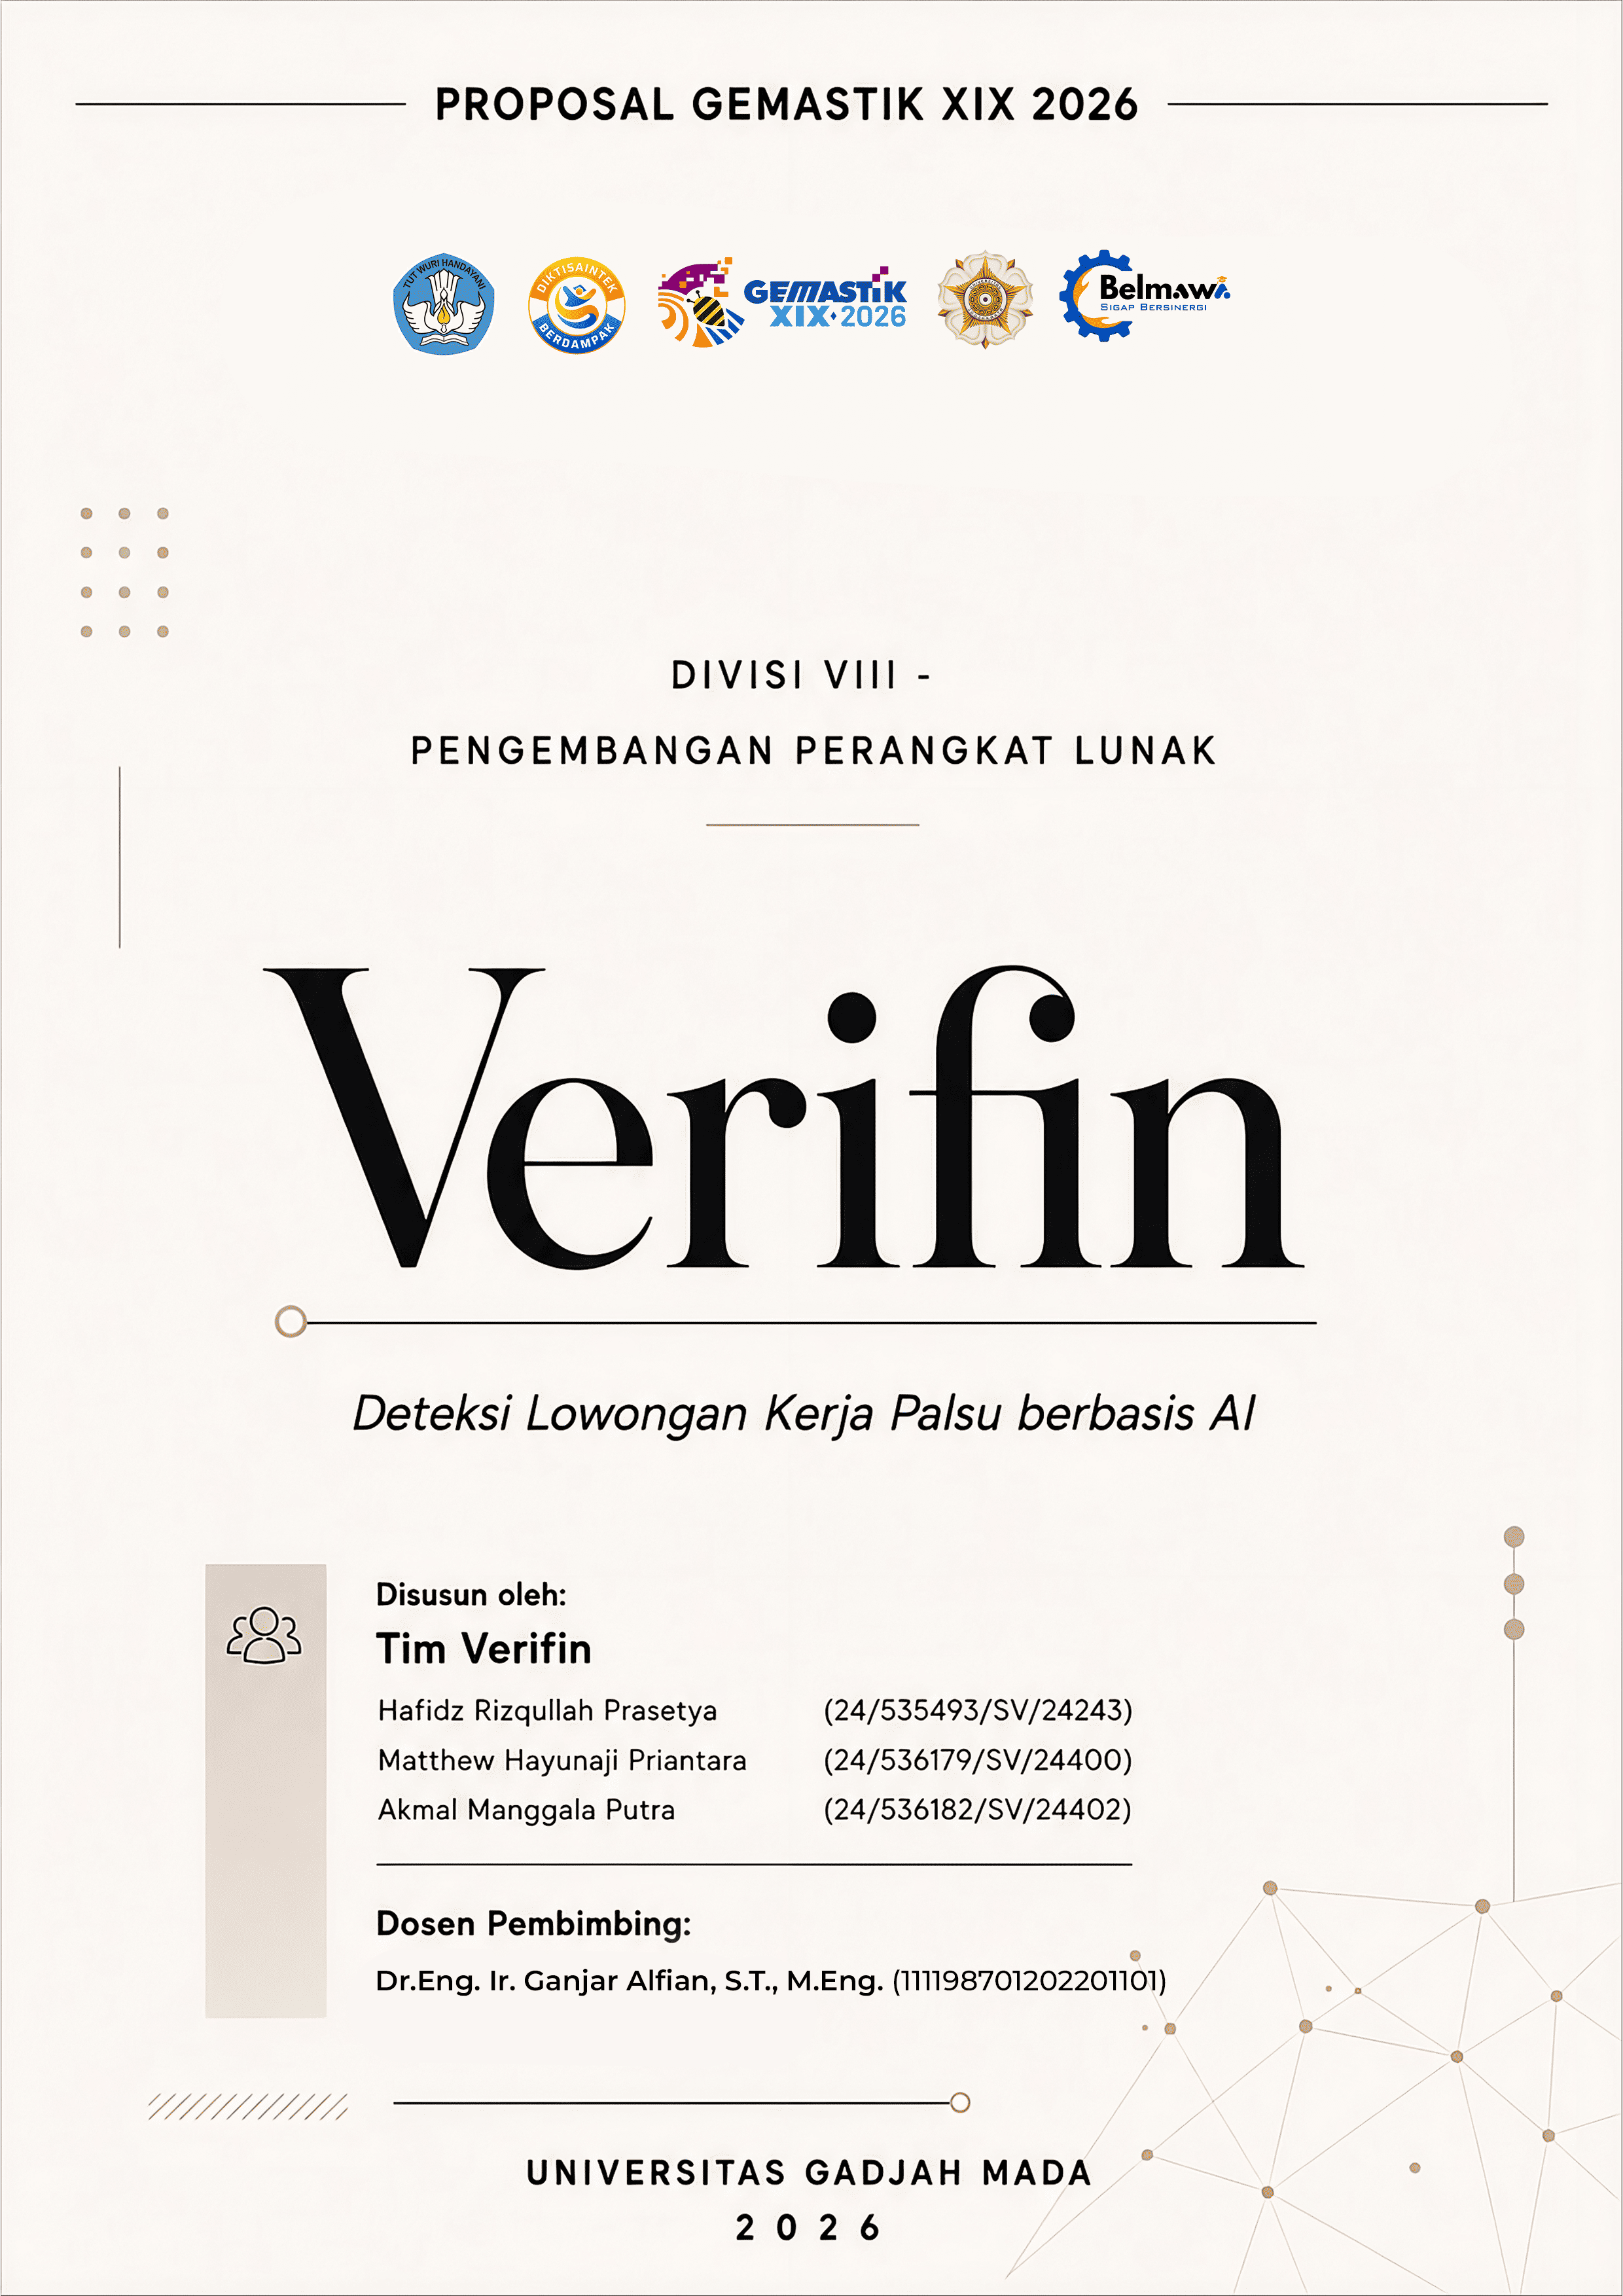
\includegraphics[width=\paperwidth,height=\paperheight]{cover.png}
  };
\end{tikzpicture}
\end{titlepage}

\newpage
\pagenumbering{roman}
\renewcommand{\contentsname}{DAFTAR ISI}
\tableofcontents
\newpage
\pagenumbering{arabic}

\refstepcounter{section}
\section*{BAB I\quad LATAR BELAKANG}
\addcontentsline{toc}{section}{BAB I LATAR BELAKANG}

\subsection*{A.\quad Urgensi Masalah dan Skenario Pengguna}
\addcontentsline{toc}{subsection}{A. Urgensi Masalah dan Skenario Pengguna}

Tingkat pengangguran terbuka di Indonesia masih menjadi salah satu tantangan ekonomi nasional yang
signifikan. Berdasarkan Berita Resmi Statistik Badan Pusat Statistik (BPS) No.\ 39/05/Th.\ XXVIII,
per Februari 2025 jumlah pengangguran terbuka tercatat mencapai 7,28 juta orang (TPT 4,76\%),
meningkat dari 7,20 juta orang pada periode yang sama tahun sebelumnya [1]. Di tengah tekanan
tersebut, jutaan pencari kerja Indonesia setiap harinya menerima tawaran lowongan dari berbagai
kanal yang tidak terkurasi: Instagram, WhatsApp, Telegram, grup Facebook, hingga papan pengumuman
fisik. Laporan \textit{State of Scams in Indonesia} oleh Global Anti-Scam Alliance (GASA) bersama
Mastercard menunjukkan skala persoalan ini: 66\% orang dewasa di Indonesia terekspos setidaknya
satu upaya penipuan digital dalam 12 bulan terakhir, dengan total estimasi kerugian finansial
nasional mencapai Rp49 triliun [2]. Dari seluruh korban penipuan digital, \textbf{49\% di antaranya
terekspos modus penipuan lowongan kerja (\textit{employment scam})}, menjadikannya salah satu
modus paling dominan [2]. Lebih jauh, krisis ini tidak berhenti pada kerugian finansial.
Kementerian Luar Negeri RI mencatat lebih dari 3.300 WNI diselamatkan dari pusat-pusat
\textit{online scamming} di Asia Tenggara (Kamboja, Myanmar, Laos, Filipina) pada periode
2020--2024, yang keseluruhannya berangkat akibat tergiur iklan lowongan kerja palsu di media
sosial [3]. Temuan ini sejalan dengan laporan UNODC yang menegaskan bahwa penipuan rekrutmen daring
(\textit{fraudulent job postings}) merupakan metode utama perekrutan korban Tindak Pidana
Perdagangan Orang (TPPO) untuk dipekerjakan paksa di \textit{cyber scam centers} [4].

Di balik fakta-fakta tersebut, terdapat satu persoalan mendasar: \textbf{pencari kerja harus
memverifikasi keaslian tawaran secara mandiri} dari berbagai sumber yang tersebar --- mencari nama
perusahaan di mesin pencari, mengecek reputasi nomor kontak, memvalidasi alamat di peta digital,
hingga memeriksa legalitas badan usaha. Proses ini memerlukan waktu dan literasi digital yang
memadai, sehingga sering kali tidak dilakukan sebelum pengguna mengambil keputusan. Kondisi ini
menciptakan \textbf{kesenjangan informasi (\textit{information asymmetry})} yang tajam antara
pembuat tawaran dan penerima tawaran, tepat pada momen ketika penerima berada dalam posisi paling
rentan.

\vspace{0.1cm}
\textbf{Ilustrasi Skenario Pengguna.} Untuk membumikan persoalan di atas, perhatikan dua persona
representatif pada Gambar~\ref{fig:persona} berikut.

\begin{figure}[H]
\centering
\begin{adjustwidth}{0.50cm}{0pt}
\begin{tcbraster}[raster columns=2, raster equal height=rows, raster column skip=4mm,
  enhanced, colback=verfinblue!4, colframe=verfinblue!55, colbacktitle=verfinblue!85,
  coltitle=white, fonttitle=\bfseries\footnotesize, left=2mm, right=2mm, top=1.2mm,
  bottom=1.2mm, boxrule=0.6pt, arc=1.5mm, title filled]
\begin{tcolorbox}[title={Persona 1 \,\textbullet\, Andri (22)}]
\footnotesize
\textit{Fresh graduate di Yogyakarta.}
\smallskip

Menerima \textit{broadcast} WhatsApp:
\begin{tcolorbox}[colback=white, colframe=verfinblue!25, boxrule=0.4pt, arc=1mm,
  left=1.5mm, right=1.5mm, top=0.8mm, bottom=0.8mm]
\itshape\footnotesize ``Dibutuhkan Admin Online WFH, gaji 8--15 juta/bulan, tanpa pengalaman,
langsung kerja. Kirim foto KTP \& data diri ke nomor ini.''
\end{tcolorbox}
Desakan ekonomi membuat Andri ingin segera merespons. Untuk memverifikasi, ia harus mencari nama
``perusahaan'' di Google, mengecek nomor penghubung, memvalidasi alamat kantor, dan memastikan
legalitas; proses yang tidak ia kuasai dan memakan waktu. Tanpa alat bantu, Andri berisiko
menyerahkan KTP-nya (pintu pencurian identitas) dalam hitungan menit setelah menerima pesan.
\end{tcolorbox}
\begin{tcolorbox}[title={Persona 2 \,\textbullet\, Sari (27)}]
\footnotesize
\textit{Pencari kerja paruh waktu.}
\smallskip

Menemukan poster lowongan menarik di Instagram:
\begin{tcolorbox}[colback=white, colframe=verfinblue!25, boxrule=0.4pt, arc=1mm,
  left=2mm, right=2mm, top=0.8mm, bottom=0.8mm]
\itshape\footnotesize ``Isi Google Form berikut untuk mendaftar. Cantumkan data pribadi lengkap
dan nomor HP aktif.''
\end{tcolorbox}
Sari tidak tahu bahwa formulir tersebut bukan milik perusahaan resmi. Tidak ada cara baginya
memastikan apakah jejak digital ``perusahaan'' itu asli atau baru dibuat kemarin, sehingga data
pribadinya berisiko masuk ke basis phishing.
\end{tcolorbox}
\end{tcbraster}
\end{adjustwidth}
  \caption{Persona Pengguna Verifin}
  \label{fig:persona}
\end{figure}

\begin{adjustwidth}{0.50cm}{0pt}
\begin{tcolorbox}[colback=verfinblue!5, colframe=verfinblue!75, boxrule=0.8pt, arc=2mm, left=4mm, right=4mm, top=3mm, bottom=3mm]
\centering\small
\textcolor{verfinblue!90}{\textbf{TITIK KRITIS \& PERNYATAAN FOKUS VERIFIN}} \\[3pt]
\itshape ``Pengguna dipaksa mengambil keputusan sebelum memiliki informasi yang cukup, dan tidak ada alat yang melakukan verifikasi terintegrasi atas nama mereka.''
\end{tcolorbox}
\end{adjustwidth}

Solusi yang sudah ada belum menjawab kesenjangan ini. Platform media sosial hanya menyediakan
fitur pelaporan reaktif; job board formal terbatas pada perusahaan yang membayar; imbauan
pemerintah bersifat umum. \textbf{Tidak ada mekanisme verifikasi terintegrasi} yang mampu
menganalisis tawaran kerja dan memberikan penilaian berbasis bukti kepada pengguna
\textit{sebelum} mereka merespons. Verifin dirancang untuk mengisi celah tersebut.

\begin{adjustwidth}{0.50cm}{0pt}
\begin{tcolorbox}[colback=verfingreen!5, colframe=verfingreen!60, boxrule=0.8pt, arc=2mm, left=4mm, right=4mm, top=3mm, bottom=3mm]
\centering\small
\textcolor{verfingreen!70!black}{\textbf{KONTRIBUSI INOVATIF VERIFIN}} \\[3pt]
\begin{minipage}{\linewidth}
\small
\begin{enumerate}[label=\textbf{\arabic*.}, leftmargin=0.6cm, itemsep=2pt]
\item \textbf{Verifikasi proaktif pertama} pada titik penerimaan lowongan di kanal informal Indonesia, menggantikan proses investigasi manual yang tersebar menjadi satu analisis terpadu.
\item \textbf{XAI hibrida yang dikalibrasi untuk pola penipuan Indonesia}, menggabungkan bukti OSINT objektif dan penalaran LLM dengan kontribusi terukur per-faktor.
\item \textbf{Fraud Network Graph} untuk intelijen kolektif: setiap entitas mencurigakan yang tercatat memperkuat deteksi bagi seluruh pengguna berikutnya.
\end{enumerate}
\end{minipage}
\end{tcolorbox}
\end{adjustwidth}

\subsection*{B.\quad Posisi dan Ruang Lingkup Verifin}
\addcontentsline{toc}{subsection}{B. Posisi dan Ruang Lingkup Verifin}

\textbf{Verifin} (\textit{Verifikasi Lowongan Kerja}) adalah sebuah \textbf{\textit{Explainable
AI-powered Decision Support System} (DSS)} untuk verifikasi awal tawaran kerja pada kanal digital
informal. Sistem menganalisis teks atau URL lowongan kerja secara otomatis menggunakan rantai
teknologi berlapis: Named Entity Recognition (NER) hibrida, investigasi
OSINT multi-sumber, penalaran naratif LLM (yang sekaligus menilai sinyal perilaku teks), dan
penjelasan kontribusi bukti berbasis Explainable
AI (XAI).
Keluaran sistem adalah sebuah \textit{Skor Risiko} 0--100 (0 = sangat aman, 100 = sangat berbahaya)
beserta verdict tiga tingkat (\textbf{AMAN}/\textbf{WASPADA}/\textbf{BAHAYA}) yang didukung penjelasan berbasis bukti yang
dapat diverifikasi oleh pengguna awam.

Secara ringkas, kontribusi utama Verifin dapat dinyatakan dalam satu kalimat:

\begin{quote}
\itshape ``Kami mengembangkan \textit{Explainable AI-powered Decision Support System} yang
mengintegrasikan OSINT dan analisis linguistik untuk mengurangi kesenjangan informasi
(\textit{information asymmetry}) pada tahap verifikasi awal tawaran kerja di kanal informal.''
\end{quote}

Verifin mengintervensi satu penyebab utama yang dapat diselesaikan melalui
rekayasa perangkat lunak, yaitu \textit{information asymmetry} pada tahap verifikasi awal. Sebagai
\textit{decision support system}, keputusan akhir tetap berada di tangan pengguna; Verifin
bertugas memastikan keputusan tersebut diambil dengan informasi yang lengkap, transparan, dan
dapat diaudit.

\subsection*{C.\quad Perbandingan dengan Solusi yang Sudah Ada}
\addcontentsline{toc}{subsection}{C. Perbandingan dengan Solusi yang Sudah Ada}

Untuk menegaskan orisinalitas dan posisi Verifin, berikut perbandingan dengan solusi yang saat ini
tersedia bagi pencari kerja Indonesia. Tidak satu pun solusi eksisting yang melakukan
\textbf{verifikasi proaktif berbasis bukti pada titik penerimaan lowongan}; celah inilah yang diisi
Verifin.

\begin{adjustwidth}{0.50cm}{0pt}
\begin{table}[H]
\centering
\caption{Perbandingan Verifin dengan solusi verifikasi lowongan yang sudah ada}
\label{tab:perbandingan}
\vspace{0.1cm}
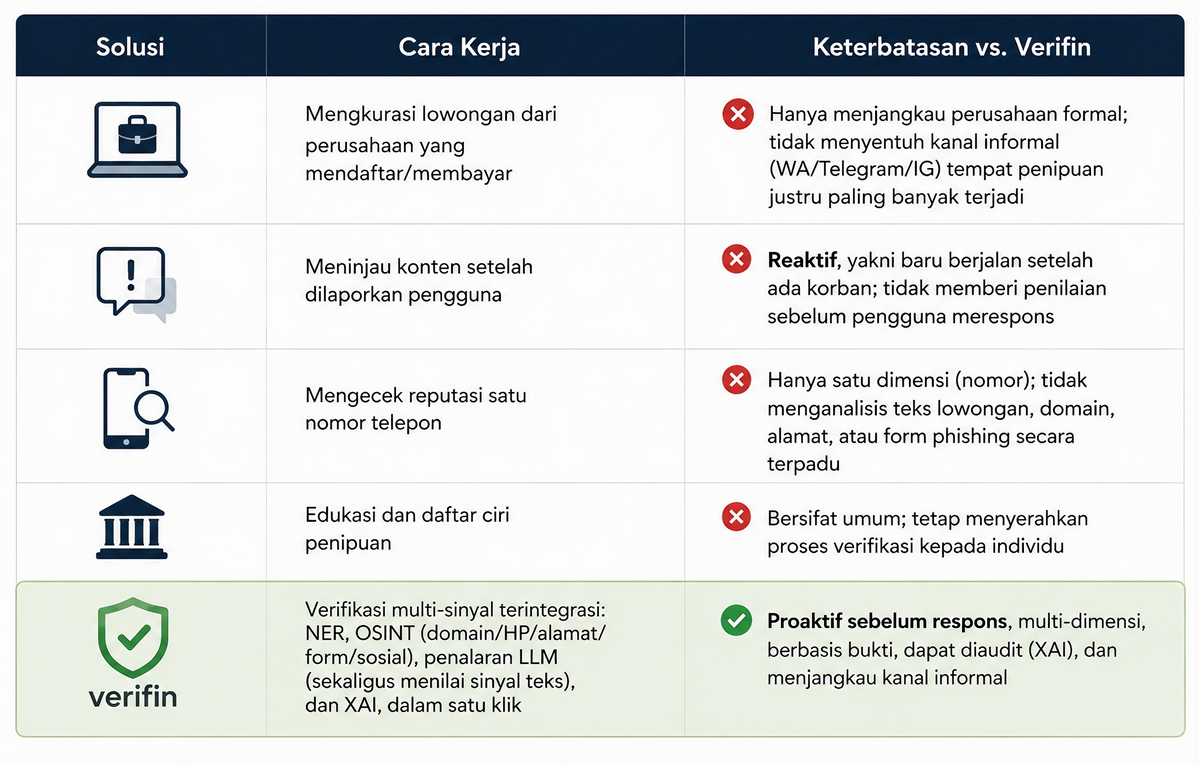
\includegraphics[width=0.72\linewidth]{images/1.1.png}
\end{table}
\end{adjustwidth}

Dari tabel di atas terlihat bahwa Verifin bersifat \textbf{komplementer, bukan duplikatif}: ia
mengintegrasikan dimensi-dimensi yang selama ini terfragmentasi (nomor, domain, alamat, media
sosial, form) menjadi satu penilaian terpadu yang \emph{dapat dioperasikan pengguna awam} tepat
pada momen pengambilan keputusan.

\vspace{0.1cm}
\subsection*{D.\quad Relevansi dengan Tema GEMASTIK XIX 2026}
\addcontentsline{toc}{subsection}{D. Relevansi dengan Tema GEMASTIK XIX 2026}

Verifin secara langsung menjawab tema GEMASTIK 2026, \textit{``Berdampak, Inklusif, dan
Berkelanjutan menuju Masyarakat Cerdas''}, dengan memanfaatkan kombinasi teknologi AI
yang relevan: NER berbahasa Indonesia, OSINT otomatis, penalaran LLM API, dan XAI untuk
transparansi. Sistem ini menjawab permasalahan nyata pada bidang \textbf{pemberdayaan masyarakat
dan ekonomi kreatif}, yaitu membantu pencari kerja menilai keaslian lowongan sebelum merespons,
dan merupakan perangkat lunak fungsional yang \textbf{dapat
dioperasikan dan dampaknya terukur} bagi masyarakat luas.

\vspace{0.1cm}

% Infografis: Statistik Kerentanan
\begin{figure}[H]
\centering
\begin{adjustwidth}{0.50cm}{0pt}
\begin{subfigure}[t]{0.55\linewidth}
\centering
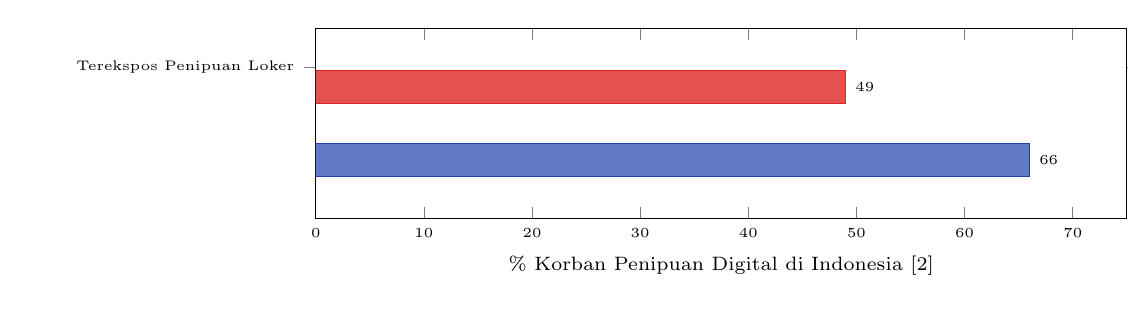
\begin{tikzpicture}
\begin{axis}[
    xbar,
    bar width=12pt,
    width=0.98\linewidth,
    height=4.0cm,
    enlarge y limits=0.35,
    xlabel={\scriptsize \% Korban Penipuan Digital di Indonesia [2]},
    symbolic y coords={Terekspos Penipuan Digital, Terekspos Penipuan Loker},
    ytick=data,
    nodes near coords,
    nodes near coords align={horizontal},
    every node near coord/.append style={font=\tiny\bfseries},
    tick label style={font=\tiny},
    label style={font=\tiny},
    xmin=0, xmax=75,
]
\addplot[fill=verfinred!80,draw=verfinred] coordinates {(49,Terekspos Penipuan Loker)};
\addplot[fill=verfinblue!70,draw=verfinblue] coordinates {(66,Terekspos Penipuan Digital)};
\end{axis}
\end{tikzpicture}
\end{subfigure}\hfill
\begin{subfigure}[t]{0.40\linewidth}
\centering
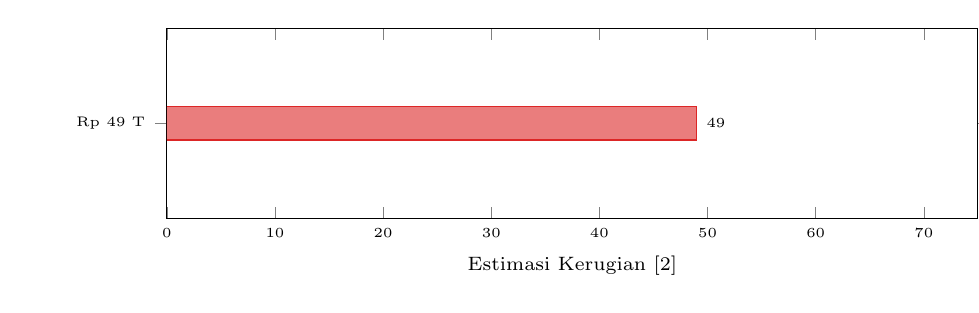
\begin{tikzpicture}
\begin{axis}[
    xbar,
    bar width=12pt,
    width=0.98\linewidth,
    height=4.0cm,
    enlarge y limits=0.35,
    xlabel={\scriptsize Estimasi Kerugian [2]},
    symbolic y coords={Rp 49 T},
    ytick=data,
    nodes near coords,
    nodes near coords align={horizontal},
    every node near coord/.append style={font=\tiny\bfseries},
    tick label style={font=\tiny},
    label style={font=\tiny},
    xmin=0, xmax=75,
]
\addplot[fill=verfinred!60,draw=verfinred] coordinates {(49,Rp 49 T)};
\end{axis}
\end{tikzpicture}
\end{subfigure}
\end{adjustwidth}
  \caption{Statistik Urgensi Penipuan Lowongan Kerja di Indonesia [2]}
  \label{fig:urgensi-stat}
\end{figure}


\refstepcounter{section}
\section*{BAB II\quad TUJUAN DAN MANFAAT}
\addcontentsline{toc}{section}{BAB II TUJUAN DAN MANFAAT}

\subsection*{A.\quad Tujuan}
\addcontentsline{toc}{subsection}{A. Tujuan}

\begin{enumerate}[label=\textbf{\arabic*.}]
\item Membangun platform web \textbf{Verifin} sebagai \textit{Explainable AI-powered Decision
      Support System} yang mampu menganalisis teks atau URL lowongan kerja secara otomatis dan
      menghasilkan \textit{Skor Risiko} 0--100 (0 = aman, 100 = berbahaya) beserta verdict
      \textbf{AMAN}\allowbreak/\textbf{WASPADA}\allowbreak/\textbf{BAHAYA} dan penjelasan berbasis
      bukti, sehingga menggantikan proses verifikasi manual yang tersebar di banyak sumber
      menjadi satu analisis terpadu dalam hitungan menit.

\item Mengimplementasikan pipeline analisis berlapis yang mengintegrasikan Named Entity Recognition
      (NER) hibrida berbahasa Indonesia, investigasi OSINT multi-sumber
      (domain, nomor telepon, perusahaan, alamat, media sosial), penalaran naratif dan verdict
      berbasis LLM (yang sekaligus menilai sinyal perilaku teks), serta penjelasan kontribusi
      bukti berbasis XAI hibrida.

\item Membangun \textit{Fraud Network Graph} berbasis database PostgreSQL yang dapat mendeteksi
      penggunaan ulang entitas-entitas mencurigakan (nomor telepon, domain, nama perusahaan) lintas
      lowongan.

\item Menyediakan fitur \textit{community monitoring} yang memungkinkan pengguna melaporkan dan
      memberikan penilaian terhadap lowongan mencurigakan secara kolektif.

\item Menyediakan REST API publik terdokumentasi untuk memungkinkan integrasi dengan platform
      pihak ketiga.
\end{enumerate}

\subsection*{B.\quad Manfaat}
\addcontentsline{toc}{subsection}{B. Manfaat}

\begin{enumerate}[label=\textbf{\arabic*.}]
\item \textbf{Bagi Pencari Kerja:} Mendapat alat verifikasi gratis, cepat, dan berbasis bukti yang
      mengurangi risiko menjadi korban penipuan lowongan. Tidak perlu lagi melakukan investigasi
      manual yang melelahkan.

\item \textbf{Bagi Ekosistem Ketenagakerjaan:} Menyediakan lapisan pendeteksi tambahan melalui
      \textit{Fraud Network Graph}. Setiap analisis baru menambah catatan entitas mencurigakan
      yang dapat dimanfaatkan untuk verifikasi berikutnya.

\item \textbf{Bagi Masyarakat Luas:} Berkontribusi dalam penanggulangan TPPO berbasis
      rekrutmen siber dengan memutus rantai penipuan di tahap paling awal, yaitu sebelum
      korban merespons iklan.

\item \textbf{Bagi Pengembang dan Peneliti:} API publik memungkinkan integrasi ke dalam platform
      lain (ekstensi browser, bot Telegram, job board). Data agregat dari sistem dapat menjadi
      sumber penelitian tentang pola penipuan kerja di Indonesia.

\item \textbf{Bagi Institusi Pendidikan dan Platform Karier:} Verifin dapat diintegrasikan sebagai
      lapisan verifikasi keamanan pada platform karier kampus (seperti UGM Career) dan job board
      nasional, meningkatkan kepercayaan pengguna dan melindungi reputasi institusi dari
      penayangan lowongan penipuan.
\end{enumerate}

\subsection*{C.\quad Estimasi Dampak Kuantitatif}
\addcontentsline{toc}{subsection}{C. Estimasi Dampak Kuantitatif}

Sesuai aspek penilaian bahwa dampak \emph{harus dibuktikan dengan data} dan produk harus
\emph{dapat dioperasikan sehingga dampak terukur}, kami menyusun estimasi dampak kuantitatif
berikut. Estimasi ini bersifat \textbf{proyeksi konservatif berbasis data sekunder resmi}
dengan asumsi yang dinyatakan secara eksplisit agar dapat diaudit.

\begin{enumerate}[label=\textbf{\arabic*.}]
\item \textbf{Populasi yang dapat dilayani:} Dengan 7,28 juta pengangguran terbuka [1] dan fakta
bahwa 49\% korban penipuan digital terekspos modus lowongan kerja [2], terdapat jutaan pencari
kerja yang merupakan calon pengguna Verifin pada kanal informal (WhatsApp, Telegram, Instagram).
Setiap verifikasi yang dilakukan pengguna secara langsung \textbf{mengurangi kesenjangan informasi}
pada momen paling rentan sebelum mereka merespons tawaran.

\item \textbf{Estimasi potensi penurunan risiko:} Bila dalam satu siklus awal Verifin memproses
$N$ verifikasi dan proporsi lowongan berisiko yang terdeteksi \textbf{BAHAYA}/\textbf{WASPADA}
adalah $p$, maka terdapat $N \times p$ pengguna yang \textbf{diperingatkan sebelum mentransfer
uang atau menyerahkan data pribadi}. Mengacu pada rata-rata kerugian penipuan daring
per korban pada laporan GASA [2], setiap kasus yang berhasil dicegah setara dengan
penghindaran kerugian finansial. Sebagai gambaran perhitungan (bukan hasil pengukuran): bila pada
1.000 verifikasi diasumsikan 20\% terindikasi berisiko dan 30\% di antaranya memilih tidak
melanjutkan setelah diperingatkan, maka terdapat 60 pengguna yang terhindar
dari tindakan berisiko. Angka ini merupakan proyeksi konservatif dengan asumsi eksplisit, dan akan
divalidasi melalui studi pengguna.

\item \textbf{Dampak kolektif melalui Fraud Network Graph:} Setiap entitas mencurigakan yang
tercatat dapat memperkuat deteksi bagi pengguna berikutnya (\textit{network effect}).

\item \textbf{Kontribusi pada penanggulangan TPPO:} Mengingat penipuan rekrutmen daring adalah
metode utama perekrutan korban TPPO ke \textit{cyber scam centers} [3], [4], intervensi Verifin
pada tahap awal, yaitu sebelum korban merespons iklan, dapat membantu memutus rantai
perdagangan orang pada titik yang dapat diotomatisasi oleh perangkat lunak.

\item \textbf{Keberlanjutan (\textit{sustainability}):} Model dampak di atas berkelanjutan karena
(a) biaya marginal per verifikasi rendah (infrastruktur web + LLM API), (b) nilai sistem meningkat
seiring pertumbuhan basis data komunitas, dan (c) API publik memungkinkan integrasi ke kanal lain
(ekstensi peramban, bot WhatsApp/Telegram) tanpa mengubah inti sistem.
\end{enumerate}

\subsection*{D.\quad Rencana Kemitraan Strategis dan Pilot Deployment}
\addcontentsline{toc}{subsection}{D. Rencana Kemitraan Strategis dan Pilot Deployment}

Untuk memastikan Verifin tidak berhenti sebagai prototipe, kami merancang strategi
\textit{go-to-market} melalui kemitraan institusional yang konkret.

\begin{enumerate}[label=\textbf{\arabic*.}]
\item \textbf{Kemitraan UGM Career (Kantor Alumni UGM):} Verifin direncanakan untuk diintegrasikan
sebagai lapisan verifikasi keamanan pada platform UGM Career
(\url{https://alumni.ugm.ac.id/ugmcareer/}) yang melayani ribuan mahasiswa dan alumni UGM.
Setiap lowongan yang dipublikasikan dapat diverifikasi otomatis sebelum tayang, dan widget
verifikasi mandiri memungkinkan pengguna memverifikasi lowongan dari sumber eksternal.
Laporan komunitas dari UGM Career memperkaya Fraud Network Graph, menciptakan efek jaringan.

\item \textbf{Pilot user study terkontrol:} Bekerjasama dengan UGM Career, kami merencanakan
\textit{pilot user study} dengan desain kontrol--perlakuan pada mahasiswa tingkat akhir
dan \textit{fresh graduate}. Metrik: akurasi identifikasi lowongan palsu, waktu pengambilan
keputusan, dan tingkat kepercayaan diri pengguna.

\item \textbf{Skala nasional melalui API publik:} REST API Verifin memungkinkan integrasi oleh
job board nasional, platform pemerintah (Kemnaker, Kartu Prakerja), maupun kanal komunitas
(bot WhatsApp/Telegram).
\end{enumerate}


\refstepcounter{section}
\section*{BAB III\quad BATASAN}
\addcontentsline{toc}{section}{BAB III BATASAN}

\subsection*{A.\quad Bahasa Input}
\addcontentsline{toc}{subsection}{A. Bahasa Input}
Sistem dioptimalkan untuk memproses teks lowongan dalam Bahasa Indonesia. Input dalam bahasa
lain (Inggris, campuran) dapat diterima karena penalaran LLM bersifat toleran
bahasa, namun akurasi NER dan kelengkapan bukti OSINT tidak dijamin setara.

\subsection*{B.\quad Sumber OSINT}
\addcontentsline{toc}{subsection}{B. Sumber OSINT}
Investigasi OSINT terbatas pada sumber yang dapat diakses secara publik dan legal:
\begin{enumerate}[label=\textbf{\arabic*.}]
  \item Whois lookup untuk domain (usia \& registrar domain) serta keamanan email (SPF/DMARC)
  \item Reputasi nomor telepon Indonesia via \textbf{Kaspersky Who Calls} dan pencarian
        laporan penipuan pada \textbf{SERP publik}
  \item Validasi alamat fisik dan keberadaan bisnis pada peta via OpenStreetMap (\textbf{Nominatim})
  \item Pencarian jejak digital perusahaan via metasearch \textbf{SearXNG} multi-engine
        (DuckDuckGo, Mojeek, Startpage, Brave) dengan filter relevansi entitas, ditunjang
        peramban ringan Lightpanda sebagai cadangan
  \item Inspeksi formulir/shortlink (Google Form) untuk deteksi phishing dan permintaan dokumen sensitif
  \item Penelusuran media sosial publik (Instagram, Facebook, LinkedIn) dengan filter profil-resmi
\end{enumerate}
Sistem \textbf{tidak} mengakses database kepolisian, Dukcapil, atau sistem pemerintah lainnya
yang memerlukan otorisasi khusus.

\subsection*{C.\quad Skala Database Awal}
\addcontentsline{toc}{subsection}{C. Skala Database Awal}
\textit{Fraud Network Graph} diinisialisasi dengan dataset awal yang terkurasi untuk memastikan
fungsionalitas penuh sejak hari pertama. Database komunitas berkembang secara organik setelah
sistem diluncurkan ke publik.

\subsection*{D.\quad Platform Target}
\addcontentsline{toc}{subsection}{D. Platform Target}
Verifin adalah aplikasi web yang dioptimalkan untuk desktop browser (Chrome, Firefox, Safari).
Tidak ada aplikasi mobile native dalam cakupan pengembangan ini, meskipun antarmuka bersifat
responsif untuk mobile.

\subsection*{E.\quad Strategi NLP Bahasa Indonesia}
\addcontentsline{toc}{subsection}{E. Strategi NLP Bahasa Indonesia}

Penilaian sinyal perilaku teks dilakukan oleh \textbf{penalaran LLM berbasis bukti} yang
dipandu panduan deteksi pola penipuan lowongan kerja Indonesia. Pendekatan ini dipilih karena
dataset berlabel lowongan penipuan berbahasa Indonesia belum tersedia secara publik [9],
sehingga penalaran LLM yang agnostik-bahasa menjadi solusi yang transparan dan dapat diaudit.
Verifin telah mengimplementasikan dukungan Bahasa Indonesia yang substantif: NER hibrida
dirancang khusus untuk pola Indonesia (nomor telepon, alamat, format gaji Rupiah, nama
perusahaan), OCR dikonfigurasi dengan model Bahasa Indonesia, dan panduan deteksi dikurasi
dari pola penipuan aktual di Indonesia. Data laporan komunitas yang terkumpul akan menjadi
korpus berlabel pertama untuk domain ini, menjadi dasar \textit{fine-tuning} model IndoBERT
pada agenda pengembangan lanjutan.

\subsection*{F.\quad Ketergantungan API Eksternal}
\addcontentsline{toc}{subsection}{F. Ketergantungan API Eksternal}
Pipeline analisis bergantung pada layanan eksternal (API LLM untuk penalaran dan Supabase
untuk database). Gangguan pada layanan ini akan mempengaruhi ketersediaan sistem.

\subsection*{G.\quad Bukan Layanan Hukum}
\addcontentsline{toc}{subsection}{G. Bukan Layanan Hukum}
Verdict yang dihasilkan Verifin adalah \textbf{penilaian berbasis risiko}, bukan keputusan
hukum. Sistem tidak dapat memastikan secara definitif bahwa sebuah lowongan adalah penipuan.
Pengguna tetap dianjurkan untuk melakukan verifikasi tambahan pada lowongan dengan skor
perbatasan.

\subsection*{H.\quad Privasi dan Perlindungan Data}
\addcontentsline{toc}{subsection}{H. Privasi dan Perlindungan Data}
Privasi pengguna dilindungi melalui beberapa mekanisme: (a) laporan komunitas bersifat anonim
(tanpa akun), identitas pelapor tidak diekspos ke antarmuka publik; (b) nomor telepon
ternormalisasi digunakan untuk pencocokan lintas kasus tanpa menyimpan format asli; (c) hasil
analisis disimpan untuk mendukung fitur Fraud Network dan riwayat verifikasi. Roadmap
pengembangan mencakup penerapan \textit{PII masking} sebelum pengiriman ke LLM eksternal serta
kebijakan retensi data yang lebih ketat.

\subsection*{I.\quad Batas Intervensi Sistem}
\addcontentsline{toc}{subsection}{I. Batas Intervensi Sistem}
Intervensi Verifin terbatas pada pengurangan \textit{information asymmetry} pada tahap
verifikasi awal. Faktor psikologis dan sosial korban (desakan ekonomi, bias otoritas,
\textit{social engineering}) berada di luar ruang lingkup desain sistem ini.

\subsection*{J.\quad Agenda Pengembangan Lanjutan (Future Work)}
\addcontentsline{toc}{subsection}{J. Agenda Pengembangan Lanjutan (Future Work)}
Terdapat tiga agenda pengembangan yang direncanakan setelah versi kompetisi, yakni:
\begin{enumerate}[label=\textbf{\arabic*.}]
\item \textbf{Fine-tuning model klasifikasi pada dataset lowongan penipuan Indonesia} untuk
melengkapi penalaran LLM dengan model terlatih yang representatif terhadap domain Indonesia.
\item \textbf{Studi pengguna (\textit{user study})} untuk mengukur dampak nyata Verifin terhadap kemampuan pengguna
mengidentifikasi lowongan palsu (desain kontrol--perlakuan).
\item \textbf{Integrasi kanal} melalui bot WhatsApp dan ekstensi peramban untuk menurunkan hambatan penggunaan
(\textit{friction}) lebih jauh.
\end{enumerate}


\refstepcounter{section}
\section*{BAB IV\quad METODOLOGI PENGEMBANGAN}
\addcontentsline{toc}{section}{BAB IV METODOLOGI PENGEMBANGAN}

\subsection*{A.\quad Metodologi dan Struktur Sprint}
\addcontentsline{toc}{subsection}{A. Metodologi dan Struktur Sprint}

Pengembangan Verifin menerapkan metodologi \textbf{Agile Scrum} yang diadaptasi untuk tim 3 orang, mencakup 1 sprint persiapan (Sprint 0) dan 4 sprint utama (Sprint 1--4) berdurasi masing-masing dua minggu.

\begin{adjustwidth}{0.50cm}{0pt}
\begin{table}[H]
\centering
\caption{Struktur Sprint Pengembangan Verifin}
\label{tab:sprint-structure}
\small
\begin{tabularx}{\linewidth}{@{}p{2.0cm}p{2.6cm}Y@{}}
\toprule
\rowcolor{verfinhead}\thead{Sprint} & \thead{Periode} & \thead{Target Deliverable} \\
\midrule
\rowcolor{verfinrow}
Sprint 0 & Minggu 1--2 & Riset, desain arsitektur, setup repo, konfigurasi Supabase, scaffolding Next.js dan FastAPI \\
Sprint 1 & Minggu 3--4 & Implementasi pipeline NER hibrida (regex + LLM) + panduan deteksi sinyal perilaku pada LLM, endpoint FastAPI dasar, UI input form \\
\rowcolor{verfinrow}
Sprint 2 & Minggu 5--6 & Implementasi modul OSINT (domain, phone, company), sintesis penalaran LLM, Fraud Network Graph, XAI explainer \\
Sprint 3 & Minggu 7--8 & Skor Risiko engine, Community Monitoring, riwayat analisis, API publik, UI result dashboard, visualisasi graf \\
\rowcolor{verfinrow}
Sprint 4 & Minggu 9--10 & Pengujian integrasi, optimasi performa, deployment Vercel + Dokploy (Home Server), dokumentasi, persiapan demonstrasi \\
\bottomrule
\end{tabularx}
\end{table}
\end{adjustwidth}

\subsection*{B.\quad Pembagian Peran Tim}
\addcontentsline{toc}{subsection}{B. Pembagian Peran Tim}

\begin{adjustwidth}{0.50cm}{0pt}
\begin{table}[H]
\centering
\caption{Pembagian Peran dan Tanggung Jawab Tim Verifin}
\label{tab:team-roles}
\small
\begin{tabularx}{\linewidth}{@{}p{3.8cm}p{3.2cm}Y@{}}
\toprule
\rowcolor{verfinhead}\thead{Peran} & \thead{Anggota} & \thead{Tanggung Jawab Utama} \\
\midrule
\rowcolor{verfinrow}
Tech Lead \& AI Engineer & Hafidz Rizqullah P. & Arsitektur sistem, pipeline NER + analisis teks, LLM reasoning engine, XAI, koordinasi tim \\
Backend \& OSINT Engineer & Akmal Manggala P. & FastAPI backend, modul OSINT, Fraud Network Graph, database schema, API publik \\
\rowcolor{verfinrow}
Frontend \& Integration & Matthew Hayunaji P. & Next.js frontend, UI/UX, visualisasi graf, integrasi LLM, community monitoring \\
\bottomrule
\end{tabularx}
\end{table}
\end{adjustwidth}

\subsection*{C.\quad Prinsip Pengembangan}
\addcontentsline{toc}{subsection}{C. Prinsip Pengembangan}

\begin{enumerate}[label=\textbf{\arabic*.}]
\item \textbf{API-First:} Backend dirancang sebagai API murni sehingga frontend dan pihak ketiga
      dapat mengintegrasikan layanan dengan mudah.
\item \textbf{Test-Driven:} Setiap modul pipeline dilengkapi unit test sebelum integrasi.
\item \textbf{Security by Design:} Validasi input, rate limiting, dan manajemen secret diterapkan
      sejak Sprint 0.
\item \textbf{Explainability First:} Setiap keputusan Skor Risiko harus dapat dijelaskan dengan
      kontribusi fitur yang terukur.
\item \textbf{Progressive Enhancement:} Sistem fungsional minimal tersedia di akhir setiap sprint;
      tidak ada sprint yang berakhir tanpa \textit{working software}.
\end{enumerate}

\subsection*{D.\quad Tools dan Platform Pengembangan}
\addcontentsline{toc}{subsection}{D. Tools dan Platform Pengembangan}

\begin{adjustwidth}{0.50cm}{0pt}
\begin{table}[htbp]
\centering
\caption{Tools dan Platform Pengembangan Verifin}
\label{tab:tools-platform}
\vspace{0.1cm}
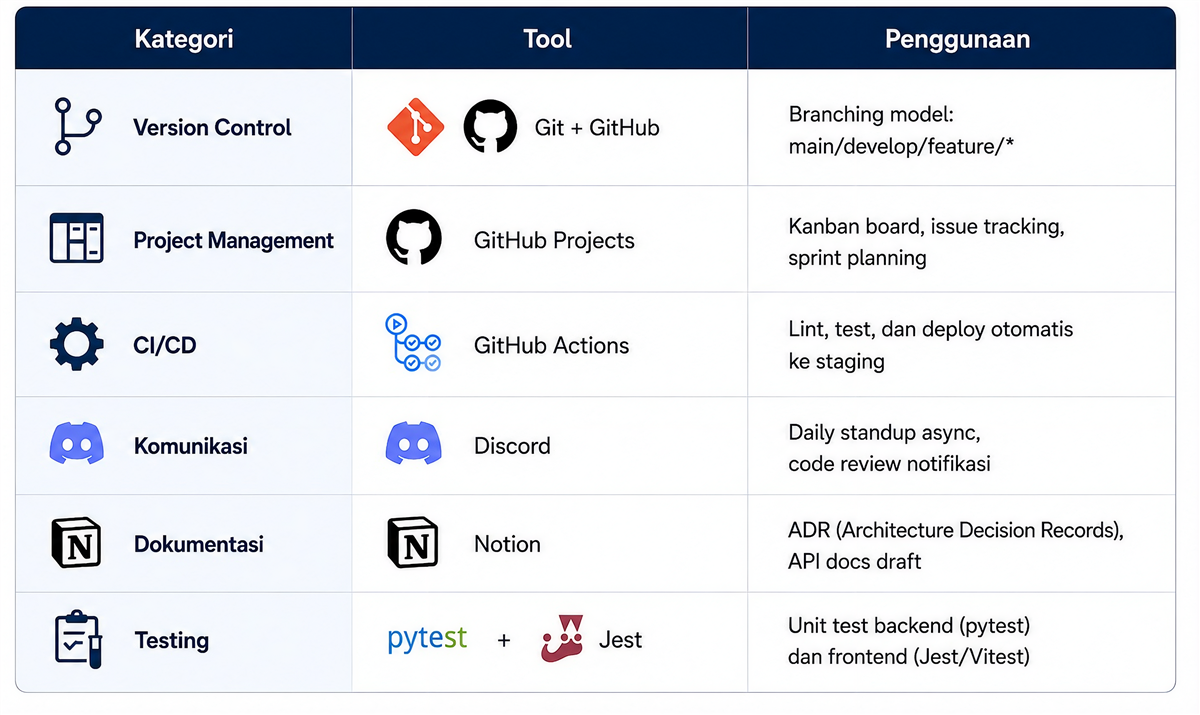
\includegraphics[width=0.70\linewidth]{images/4.3.png}
\end{table}
\end{adjustwidth}


\refstepcounter{section}
\section*{BAB V\quad ANALISIS KEBUTUHAN DAN DESAIN SOLUSI}
\addcontentsline{toc}{section}{BAB V ANALISIS KEBUTUHAN DAN DESAIN SOLUSI}

\subsection*{A.\quad Analisis Kebutuhan Fungsional}
\addcontentsline{toc}{subsection}{A. Analisis Kebutuhan Fungsional}

\begin{adjustwidth}{0.50cm}{0pt}
\begingroup
\small
\setlength{\LTleft}{0pt}
\setlength{\LTright}{0pt}
\begin{longtable}{@{}p{1.2cm}p{3.0cm}p{8.2cm}p{1.6cm}@{}}
\caption{Daftar Kebutuhan Fungsional Verifin}
\label{tab:fr-list}\\
\toprule
\rowcolor{verfinhead}\thead{ID} & \thead{Nama} & \thead{Deskripsi} & \thead{Prioritas} \\
\midrule
\endfirsthead
\multicolumn{4}{c}{\footnotesize Tabel \ref{tab:fr-list} (lanjutan)}\\
\toprule
\rowcolor{verfinhead}\thead{ID} & \thead{Nama} & \thead{Deskripsi} & \thead{Prioritas} \\
\midrule
\endhead
\midrule\multicolumn{4}{r}{\footnotesize Bersambung ke halaman berikutnya}\\
\endfoot
\bottomrule
\endlastfoot
\rowcolor{verfinrow}
FR-01 & Input Teks Lowongan & Pengguna dapat menempelkan teks lowongan kerja (min. 50 karakter) ke dalam form input dan mengirimkan untuk dianalisis & Tinggi \\
FR-02 & Input URL Lowongan & Pengguna dapat memasukkan URL halaman lowongan kerja; sistem mengekstrak teks dari halaman tersebut secara otomatis & Tinggi \\
\rowcolor{verfinrow}
FR-03 & Ekstraksi Entitas NER Hibrida & Sistem mengekstrak entitas (nama perusahaan, nomor telepon, email, URL/domain, gaji, lokasi) menggunakan kombinasi regex (entitas struktural) dan LLM (entitas semantik) & Tinggi \\
FR-04 & Penilaian Sinyal Perilaku Teks & Sistem menilai sinyal perilaku teks lowongan melalui penalaran LLM yang dipandu panduan deteksi pola penipuan Indonesia (permintaan biaya, kerja luar negeri, apply-via-WA, gaji fantastis, permintaan dokumen sensitif); bukan modul klasifikasi terpisah & Tinggi \\
\rowcolor{verfinrow}
FR-05 & Investigasi OSINT Domain & Sistem melakukan investigasi terhadap domain/URL yang ditemukan: Whois, usia domain, keaktifan website & Tinggi \\
FR-06 & Investigasi OSINT Telepon & Sistem memvalidasi format nomor telepon Indonesia dan mengecek laporan fraud via Kaspersky Who Calls serta pencarian SERP publik & Tinggi \\
\rowcolor{verfinrow}
FR-07 & Investigasi OSINT Perusahaan & Sistem mencari jejak digital perusahaan via multi-engine web search (dengan filter relevansi entitas) dan mengidentifikasi inkonsistensi dengan klaim dalam lowongan & Tinggi \\
FR-08 & Penalaran Naratif \& Verdict LLM & Sistem menghasilkan verdict \textbf{AMAN}/\textbf{WASPADA}/\textbf{BAHAYA} dan ringkasan narasi berbahasa Indonesia menggunakan LLM, secara ketat berbasis bukti OSINT (dilarang mengarang fakta di luar evidence) & Tinggi \\
\rowcolor{verfinrow}
FR-09 & Skor Risiko dan Verdict & Sistem menghasilkan Skor Risiko integer 0--100 (0 = sangat aman, 100 = sangat berbahaya) melalui agregasi kontribusi bukti XAI, beserta verdict tiga tingkat: \textbf{AMAN}, \textbf{WASPADA}, \textbf{BAHAYA} & Tinggi \\
FR-10 & Penjelasan XAI & Sistem menghasilkan penjelasan kontribusi setiap bukti terhadap Skor Risiko menggunakan SHAP-inspired additive explainer (bobot dikalibrasi dari pola penipuan Indonesia) & Tinggi \\
\rowcolor{verfinrow}
FR-11 & Visualisasi Graf Jaringan & Sistem menampilkan graf interaktif koneksi entitas lowongan dengan entitas lain di database & Sedang \\
FR-12 & Community Monitoring & Pengguna dapat melaporkan lowongan mencurigakan, memberi upvote/downvote laporan, dan melihat daftar laporan & Sedang \\
\rowcolor{verfinrow}
FR-13 & Riwayat Analisis & Sistem menyimpan riwayat analisis pengguna berdasarkan sesi/akun & Sedang \\
FR-14 & API Publik & Sistem menyediakan REST API terdokumentasi via FastAPI auto-docs untuk integrasi pihak ketiga & Sedang \\
\end{longtable}
\endgroup
\end{adjustwidth}

\subsection*{B.\quad Analisis Kebutuhan Non-Fungsional}
\addcontentsline{toc}{subsection}{B. Analisis Kebutuhan Non-Fungsional}

\begin{adjustwidth}{0.50cm}{0pt}
\begin{table}[H]
\centering
\caption{Daftar Kebutuhan Non-Fungsional Verifin}
\label{tab:nfr-list}
\small
\begin{tabularx}{\linewidth}{@{}p{1.6cm}p{3.0cm}Y@{}}
\toprule
\rowcolor{verfinhead}\thead{ID} & \thead{Nama} & \thead{Deskripsi} \\
\midrule
\rowcolor{verfinrow}
NFR-01 & Performa & Pipeline analisis lengkap (OCR $\to$ NER $\to$ OSINT paralel $\to$ LLM reasoning $\to$ XAI) ditargetkan selesai dalam 1--2 menit untuk 90\% permintaan (latensi didominasi sintesis LLM). Modul OSINT dijalankan paralel untuk meminimalkan waktu tunggu, dan pengguna diberi indikator progres bertahap selama analisis berjalan. \\
NFR-02 & Ketersediaan & Uptime minimal 95\% selama periode demonstrasi dan evaluasi. \\
\rowcolor{verfinrow}
NFR-03 & Keamanan & Input divalidasi dan disanitasi; API key disimpan sebagai environment variable; rate limiting pada endpoint analisis. \\
NFR-04 & Skalabilitas & Arsitektur FastAPI memungkinkan horizontal scaling; PostgreSQL di Supabase mendukung koneksi pooling. \\
\rowcolor{verfinrow}
NFR-05 & Kemudahan Penggunaan & Dapat digunakan pencari kerja awam tanpa pelatihan teknis; proses analisis cukup paste teks dan klik tombol. \\
NFR-06 & Transparansi & Setiap verdict disertai penjelasan berbasis fitur yang dapat dipahami dan diverifikasi. \\
\bottomrule
\end{tabularx}
\end{table}
\end{adjustwidth}

\subsection*{C.\quad Desain Solusi: Arsitektur Sistem}
\addcontentsline{toc}{subsection}{C. Desain Solusi: Arsitektur Sistem}

Verifin mengimplementasikan arsitektur berlapis (\textit{layered architecture}) yang memisahkan
tanggung jawab setiap komponen secara jelas. Berikut adalah diagram arsitektur sistem secara
keseluruhan:\par

\vspace{0.1cm}

% ── DIAGRAM PIPELINE 4-LAYER ──────────────────────────────────────────────
\begin{figure}[H]
\centering
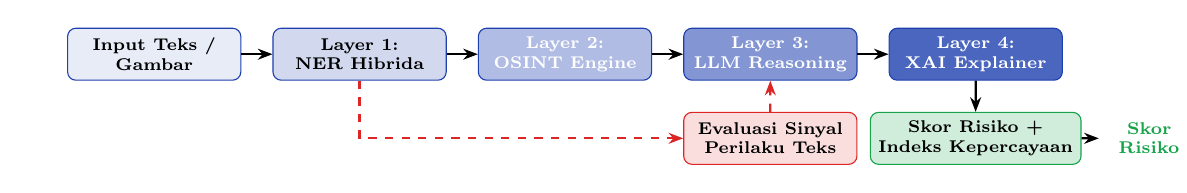
\begin{tikzpicture}[
    scale=0.88, transform shape,
    layer/.style={draw, rectangle, rounded corners=3pt, minimum width=2.5cm, minimum height=0.75cm, font=\scriptsize\bfseries, align=center},
    arrow/.style={-{Stealth[scale=0.8]}, thick},
    node distance=0.35cm and 0.45cm
]
\node[layer, fill=verfinblue!10, draw=verfinblue] (in) {Input Teks /\\Gambar};
\node[layer, fill=verfinblue!20, draw=verfinblue, right=of in] (l1) {Layer 1:\\NER Hibrida};
\node[layer, fill=verfinblue!35, draw=verfinblue, text=white, right=of l1] (l2) {Layer 2:\\OSINT Engine};
\node[layer, fill=verfinblue!55, draw=verfinblue, text=white, right=of l2] (l3) {Layer 3:\\LLM Reasoning};
\node[layer, fill=verfinblue!80, draw=verfinblue, text=white, right=of l3] (l4) {Layer 4:\\XAI Explainer};

\draw[arrow] (in) -- (l1);
\draw[arrow] (l1) -- (l2);
\draw[arrow] (l2) -- (l3);
\draw[arrow] (l3) -- (l4);

\node[layer, fill=verfinred!15, draw=verfinred, below=0.45cm of l3] (llm_eval) {Evaluasi Sinyal\\Perilaku Teks};
\draw[arrow, dashed, color=verfinred] (l1) |- (llm_eval);
\draw[arrow, dashed, color=verfinred] (llm_eval) -- (l3);

\node[layer, fill=verfingreen!20, draw=verfingreen, below=0.45cm of l4] (xai) {Skor Risiko +\\Indeks Kepercayaan};
\draw[arrow] (l4) -- (xai);
\node[right=0.25cm of xai, font=\scriptsize\bfseries, text=verfingreen, align=center, text width=1.2cm] (output) {Skor\\Risiko};
\draw[arrow] (xai) -- (output);
\end{tikzpicture}
  \caption{Arsitektur Pipeline Analisis Verifin}
  \label{fig:pipeline-verifin}
\end{figure}

\vspace{0.1cm}

% ── DIAGRAM JOB TRUST INFRASTRUCTURE ─────────────────────────────────────
\begin{figure}[H]
\centering
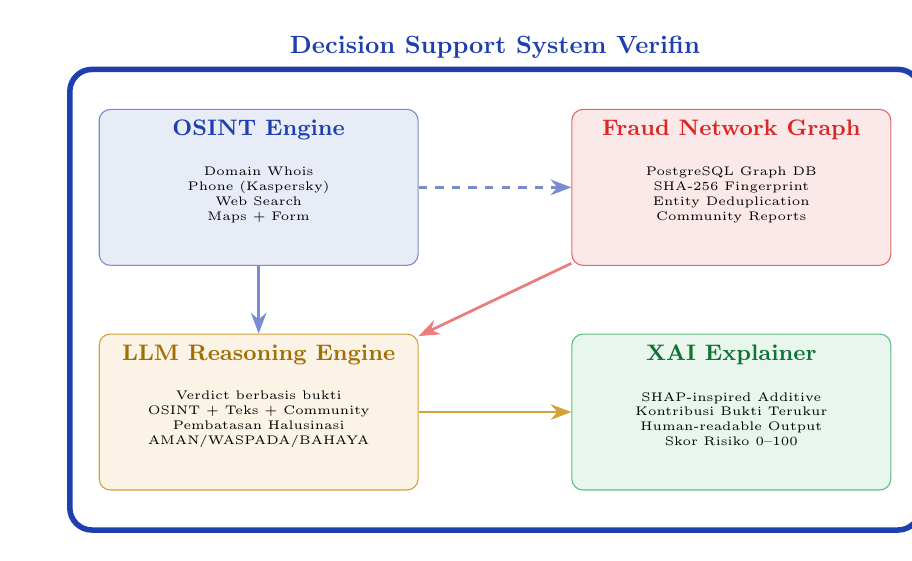
\begin{tikzpicture}[
  scale=0.90, transform shape,
  every node/.style={font=\small},
]
% Outer box — Decision Support System
\node[rectangle, draw=verfinblue, line width=2pt, rounded corners=8pt,
      minimum width=12cm, minimum height=6.5cm,
      label={[font=\bfseries\normalsize,color=verfinblue]above:Decision Support System Verifin}] (outer) {};

% Inner top-left: OSINT Engine
\node[rectangle, draw=verfinblue!60, fill=verfinblue!10, rounded corners=4pt,
      minimum width=4.5cm, minimum height=2.2cm, text centered,
      at={($(outer.north west)+(2.7cm,-1.7cm)$)}] (osint_box) {};
\node[font=\bfseries\small, color=verfinblue] at ($(osint_box.north)+(0,-0.3cm)$) {OSINT Engine};
\node[font=\tiny, align=center] at ($(osint_box.center)+(0,-0.1cm)$)
      {Domain Whois \\ Phone (Kaspersky) \\ Web Search \\ Maps + Form};

% Inner top-right: Fraud Network Graph
\node[rectangle, draw=verfinred!70, fill=verfinred!10, rounded corners=4pt,
      minimum width=4.5cm, minimum height=2.2cm, text centered,
      at={($(outer.north east)+(-2.7cm,-1.7cm)$)}] (fraud_box) {};
\node[font=\bfseries\small, color=verfinred] at ($(fraud_box.north)+(0,-0.3cm)$) {Fraud Network Graph};
\node[font=\tiny, align=center] at ($(fraud_box.center)+(0,-0.1cm)$)
      {PostgreSQL Graph DB \\ SHA-256 Fingerprint \\ Entity Deduplication \\ Community Reports};

% Inner bottom-left: Trust Scoring
\node[rectangle, draw=verfinyellow!80, fill=verfinyellow!10, rounded corners=4pt,
      minimum width=4.5cm, minimum height=2.2cm, text centered,
      at={($(outer.south west)+(2.7cm,1.7cm)$)}] (trust_box) {};
\node[font=\bfseries\small, color=verfinyellow!80!black] at ($(trust_box.north)+(0,-0.3cm)$) {LLM Reasoning Engine};
\node[font=\tiny, align=center] at ($(trust_box.center)+(0,-0.1cm)$)
      {Verdict berbasis bukti \\ OSINT + Teks + Community \\ Pembatasan Halusinasi \\ AMAN/WASPADA/BAHAYA};

% Inner bottom-right: XAI Explainer
\node[rectangle, draw=verfingreen!70, fill=verfingreen!10, rounded corners=4pt,
      minimum width=4.5cm, minimum height=2.2cm, text centered,
      at={($(outer.south east)+(-2.7cm,1.7cm)$)}] (xai_box) {};
\node[font=\bfseries\small, color=verfingreen!70!black] at ($(xai_box.north)+(0,-0.3cm)$) {XAI Explainer};
\node[font=\tiny, align=center] at ($(xai_box.center)+(0,-0.1cm)$)
      {SHAP-inspired Additive \\ Kontribusi Bukti Terukur \\ Human-readable Output \\ Skor Risiko 0--100};

% Arrows connecting components
\draw[-{Stealth}, color=verfinblue!60, line width=1pt] (osint_box) -- (trust_box);
\draw[-{Stealth}, color=verfinred!60, line width=1pt] (fraud_box) -- (trust_box);
\draw[-{Stealth}, color=verfinyellow!80, line width=1pt] (trust_box) -- (xai_box);
\draw[-{Stealth}, color=verfinblue!60, dashed, line width=1pt] (osint_box) -- (fraud_box);
\end{tikzpicture}
  \caption{Komponen Inti Decision Support System Verifin}
  \label{fig:dss-verifin}
\end{figure}

\vspace{0.1cm}

% ── DIAGRAM VERDICT TIERS ─────────────────────────────────────────────────
\begin{figure}[H]
\centering
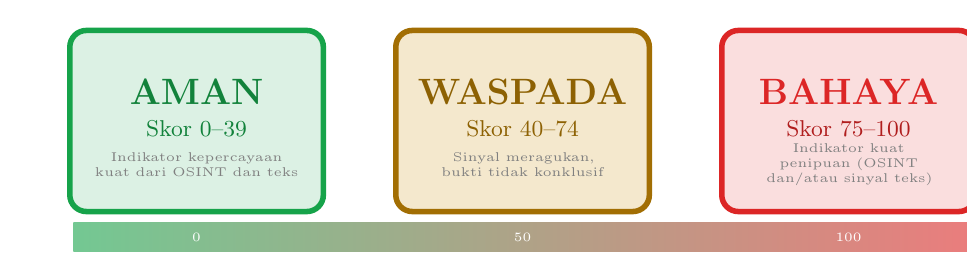
\begin{tikzpicture}[
  scale=0.92, transform shape,
  every node/.style={font=\normalsize}
]
% AMAN box (skor risiko rendah)
\node[rectangle, draw=verfingreen, fill=verfingreen!15, line width=2pt, rounded corners=6pt,
      minimum width=3.5cm, minimum height=2.5cm, text centered] (aman) at (0,0) {};
\node[font=\Large\bfseries, color=verfingreen!80!black] at ($(aman.center)+(0,0.4cm)$) {AMAN};
\node[font=\small, color=verfingreen!80!black] at ($(aman.center)+(0,-0.1cm)$) {Skor 0--39};
\node[font=\tiny, color=gray, text width=3cm, align=center] at ($(aman.center)+(0,-0.6cm)$)
      {Indikator kepercayaan kuat dari OSINT dan teks};

% WASPADA box
\node[rectangle, draw=verfinyellow!80!black, fill=verfinyellow!20, line width=2pt, rounded corners=6pt,
      minimum width=3.5cm, minimum height=2.5cm, text centered] (waspada) at (4.5,0) {};
\node[font=\Large\bfseries, color=verfinyellow!70!black] at ($(waspada.center)+(0,0.4cm)$) {WASPADA};
\node[font=\small, color=verfinyellow!70!black] at ($(waspada.center)+(0,-0.1cm)$) {Skor 40--74};
\node[font=\tiny, color=gray, text width=3cm, align=center] at ($(waspada.center)+(0,-0.6cm)$)
      {Sinyal meragukan, bukti tidak konklusif};

% BAHAYA box (skor risiko tinggi)
\node[rectangle, draw=verfinred, fill=verfinred!15, line width=2pt, rounded corners=6pt,
      minimum width=3.5cm, minimum height=2.5cm, text centered] (bahaya) at (9,0) {};
\node[font=\Large\bfseries, color=verfinred] at ($(bahaya.center)+(0,0.4cm)$) {BAHAYA};
\node[font=\small, color=verfinred!80!black] at ($(bahaya.center)+(0,-0.1cm)$) {Skor 75--100};
\node[font=\tiny, color=gray, text width=3cm, align=center] at ($(bahaya.center)+(0,-0.6cm)$)
      {Indikator kuat penipuan (OSINT dan/atau sinyal teks)};

% Scale bar below (kiri aman rendah → kanan bahaya tinggi)
\shade[left color=verfingreen!60, right color=verfinred!60]
      (-1.7cm,-1.8cm) rectangle (10.7cm,-1.4cm);
\node[font=\tiny, color=white] at (0,-1.6cm) {0};
\node[font=\tiny, color=white] at (4.5cm,-1.6cm) {50};
\node[font=\tiny, color=white] at (9cm,-1.6cm) {100};
\end{tikzpicture}
  \caption{Tiga Tingkat Verdict Verifin}
  \label{fig:verdict-levels}
\end{figure}

\vspace{0.1cm}

% ── SKOR RISIKO TABLE ─────────────────────────────────────────────────────
\begin{adjustwidth}{0.50cm}{0pt}
\begin{table}[H]
\centering
\caption{Tabel Skor Risiko dan Interpretasi Verdict}
\label{tab:skor-risiko}
\small
\begin{tabularx}{\linewidth}{@{}p{2.2cm}p{2.2cm}Y@{}}
\toprule
\rowcolor{verfinhead}\thead{Rentang Skor} & \thead{Verdict} & \thead{Interpretasi} \\
\midrule
0--39 & \textbf{\color{verfingreen!70!black}AMAN} & Lowongan memiliki indikator kepercayaan yang kuat: jejak digital OSINT terverifikasi (domain valid dan berumur, perusahaan ditemukan), tidak ada laporan penipuan, dan teks tidak memuat sinyal perilaku mencurigakan. \\
\rowcolor{verfinrow}
40--74 & \textbf{\color{verfinyellow!70!black}WASPADA} & Terdapat beberapa sinyal meragukan namun bukti tidak konklusif. Pengguna disarankan melakukan verifikasi tambahan sebelum merespons. \\
\rowcolor{verfinrow}
75--100 & \textbf{\color{verfinred}BAHAYA} & Terdapat indikator kuat penipuan, baik dari verifikasi OSINT (domain baru/tidak valid, nomor terlapor, perusahaan tidak ditemukan) maupun sinyal perilaku teks (permintaan biaya, dokumen sensitif, gaji fantastis). Pengguna sangat disarankan tidak merespons. \\
\bottomrule
\end{tabularx}
\end{table}
\end{adjustwidth}


\subsection*{D.\quad Desain Solusi: Tech Stack}
\addcontentsline{toc}{subsection}{D. Desain Solusi: Tech Stack}

\begin{figure}[H]
\centering
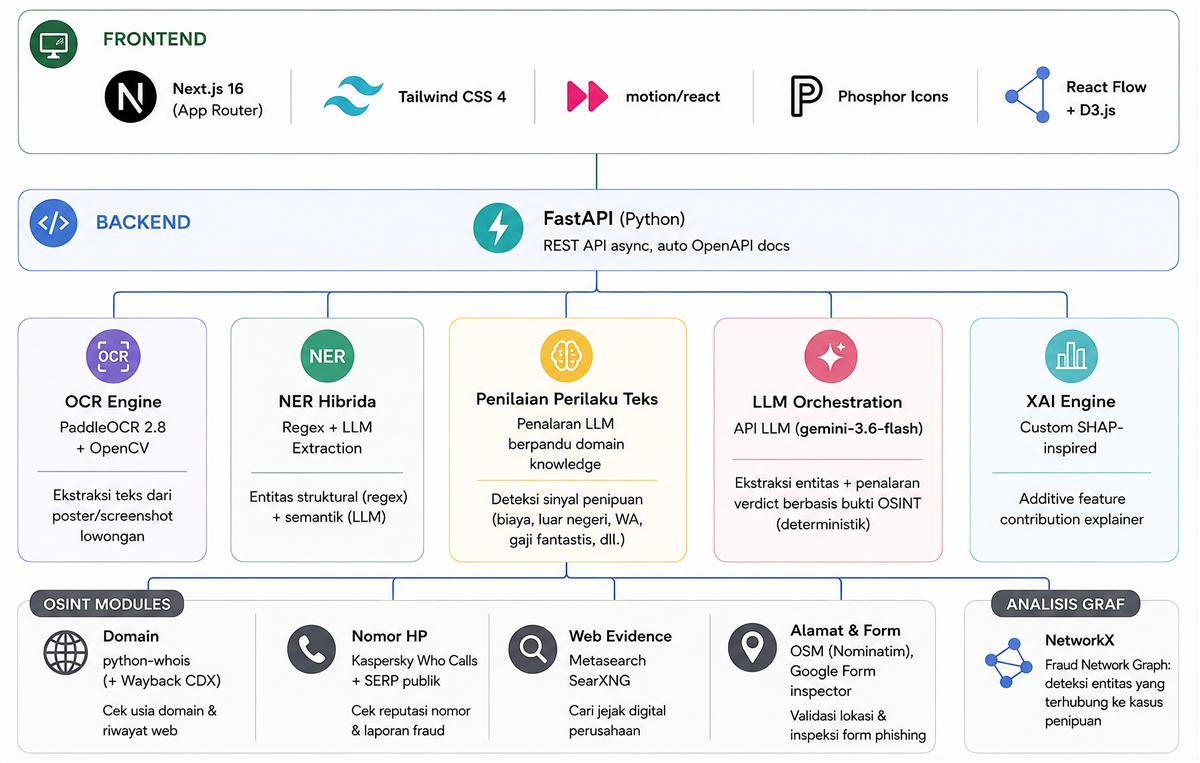
\includegraphics[width=0.75\linewidth]{images/5.4.png}
\vspace{0.1cm}
\caption{Tech Stack Verifin}
\label{fig:tech-stack}
\end{figure}


\refstepcounter{section}
\section*{BAB VI\quad IMPLEMENTASI}
\addcontentsline{toc}{section}{BAB VI IMPLEMENTASI}

\subsection*{A.\quad Implementasi Pipeline Analisis}
\addcontentsline{toc}{subsection}{A. Implementasi Pipeline Analisis}

\subsubsection*{1.\quad Layer 1: Named Entity Recognition (NER) Hibrida}
\addcontentsline{toc}{subsubsection}{1. Layer 1: Named Entity Recognition (NER) Hibrida}

\begin{adjustwidth}{1.45cm}{0pt}
\hspace*{0.85cm}Sistem mengekstrak entitas kunci dari teks lowongan menggunakan pendekatan \textbf{hibrida}
yang menggabungkan dua mekanisme komplementer:

\begin{enumerate}[label=\textbf{\alph*.}, labelindent=0pt, leftmargin=*]
\item \textbf{Regex deterministik} untuk entitas \emph{struktural} yang polanya stabil:
      nomor telepon/WhatsApp (\textbf{PHONE}), alamat surel (\textbf{EMAIL}), dan URL/domain.
      Regex cepat, murah, dan presisi-tinggi pada pola yang jelas.
\item \textbf{Ekstraksi berbasis LLM} untuk entitas \emph{semantik} yang sulit ditangkap pola
      deterministik pada poster OCR yang berantakan: nama perusahaan/organisasi (\textbf{ORG}),
      alamat fisik/lokasi kerja (\textbf{LOC}), dan informasi gaji (\textbf{SALARY}).
      LLM memahami konteks sehingga tidak rapuh terhadap variasi layout.
\end{enumerate}

Kedua mekanisme berjalan \textbf{paralel} (\textit{asyncio}). Hasil digabung dengan strategi per-kategori:
untuk \textbf{ORG}, output LLM bersifat otoritatif sehingga false-positive regex (frasa deskriptif
yang kebetulan mirip nama) otomatis tersaring; untuk \textbf{LOC} dan \textbf{SALARY}, keduanya
digabung secara aditif. Bila LLM tidak tersedia, sistem \emph{fallback} penuh ke regex sehingga
pipeline tidak pernah terputus. Output berupa JSON terstruktur yang menjadi input untuk semua
layer berikutnya.
\end{adjustwidth}

\subsubsection*{2.\quad Penilaian Sinyal Perilaku Teks oleh LLM (bukan modul terpisah)}
\addcontentsline{toc}{subsubsection}{2. Penilaian Sinyal Perilaku Teks oleh LLM}

\begin{adjustwidth}{1.45cm}{0pt}
\hspace*{0.85cm}Berbeda dari deteksi penipuan konvensional yang melatih satu model klasifikasi, Verifin
\textbf{tidak} menjalankan modul klasifikasi teks terpisah. Penilaian sinyal perilaku
(\textit{behavioral signals}) pada teks lowongan, seperti permintaan biaya/\textit{deposit},
tawaran kerja ke luar negeri (indikasi TPPO), instruksi melamar via WhatsApp, gaji fantastis
tidak realistis, serta permintaan dokumen sensitif (KTP/foto) di awal proses, dilakukan oleh
\textbf{penalaran LLM pada Layer 3} melalui prompt terstruktur yang memuat panduan deteksi pola
penipuan lowongan kerja Indonesia, terinspirasi dari daftar fitur perilaku pada penelitian
deteksi penipuan rekrutmen [5], [6]. Sinyal-sinyal ini kemudian ditimbang bersama bukti OSINT
dan dijelaskan kontribusinya pada Layer 4 (XAI). Pemilihan LLM sebagai penilai sinyal perilaku
(rather than model klasifikasi terlatih) didasarkan pada ketersediaan sumber daya NLP Bahasa
Indonesia yang telah dibahas pada BAB III.E.
\end{adjustwidth}

\subsubsection*{3.\quad Layer 2: OSINT Engine}
\addcontentsline{toc}{subsubsection}{3. Layer 2: OSINT Engine}

\begin{adjustwidth}{1.45cm}{0pt}
\hspace*{0.85cm}Modul OSINT dijalankan secara paralel menggunakan \textit{asyncio} untuk meminimalkan latensi, memanfaatkan potensi sumber informasi terbuka (OSINT) [8].
Terdapat tiga sub-modul utama:

\begin{enumerate}[label=\textbf{\alph*.}, labelindent=0pt, leftmargin=*]
\item \textbf{Domain/URL Investigator:}
\begin{enumerate}[label=\textbf{\arabic*)}, leftmargin=0.50cm]
\item Whois lookup untuk mendapatkan tanggal registrasi, registrar, dan informasi pemilik (dengan fallback ke Wayback Machine CDX bila Whois gagal)
\item Domain berumur $< 30$ hari mendapat penalti skor signifikan
\item Validasi keaktifan website (HTTP) dan kesesuaian nama domain dengan klaim perusahaan
\item Inspeksi shortlink/Google Form untuk mendeteksi pola phishing
\end{enumerate}

\item \textbf{Phone Number Validator:}
\begin{enumerate}[label=\textbf{\arabic*)}, leftmargin=0.50cm]
\item Validasi format nomor telepon Indonesia (08xx, +62xx) dengan whitelist prefix operator
\item Identifikasi operator berdasarkan prefix (Telkomsel, Indosat, XL, dll.)
\item Pengecekan reputasi dan laporan fraud via \textbf{Kaspersky Who Calls} dan pencarian \textbf{SERP publik}
\item \textit{Cross-check} nomor kontak lowongan terhadap nomor resmi bisnis yang ditemukan pada jejak publik (netral-note bila berbeda)
\end{enumerate}

\item \textbf{Company Lookup:}
\begin{enumerate}[label=\textbf{\arabic*)}, leftmargin=0.50cm]
\item Pencarian jejak digital perusahaan via metasearch \textbf{SearXNG} multi-engine dengan filter relevansi entitas (arsitektur satu query yang didistribusikan ke banyak validator, meminimalkan \textit{rate-limit})
\item Verifikasi keberadaan website resmi dan profil media sosial resmi (filter profil, bukan postingan)
\item Validasi alamat dan keberadaan bisnis pada peta via OpenStreetMap (\textbf{Nominatim})
\item Deteksi inkonsistensi antara klaim jabatan/lokasi dengan temuan publik
\end{enumerate}
\end{enumerate}
\end{adjustwidth}

\subsubsection*{4.\quad Layer 3: LLM Reasoning \& Verdict}
\addcontentsline{toc}{subsubsection}{4. Layer 3: LLM Reasoning \& Verdict}

\begin{adjustwidth}{1.45cm}{0pt}
\hspace*{0.85cm}Sistem mengirimkan bundle hasil OSINT beserta teks lowongan ke LLM
dengan prompt terstruktur. Berbeda dari penggunaan LLM konvensional yang sekadar merangkum, pada
Verifin LLM berperan sebagai \textbf{mesin penalaran (\textit{reasoning engine})} yang menimbang
seluruh bukti dan menghasilkan verdict. Pada layer ini pula LLM menilai sinyal perilaku teks
(permintaan biaya, dokumen sensitif, gaji fantastis) berdasarkan panduan deteksi pola penipuan
Indonesia. Model diinstruksikan untuk:
\begin{enumerate}[label=\textbf{\alph*.}, labelindent=0pt, leftmargin=*]
\item Menilai tingkat kepercayaan lowongan dan menetapkan verdict \textbf{AMAN}, \textbf{WASPADA}, atau \textbf{BAHAYA} beserta Skor Risiko
\item Merangkum temuan OSINT dalam narasi berbahasa Indonesia yang mudah dipahami
\item Menyebutkan fakta-fakta spesifik yang mendukung atau melemahkan kepercayaan
\item Memberikan rekomendasi tindak lanjut yang actionable
\item \textbf{Tidak membuat klaim yang tidak didukung oleh data OSINT yang tersedia}
\end{enumerate}

\textbf{Pembatasan halusinasi (\textit{hallucination guard}).} Untuk menjaga verdict tetap berbasis bukti, LLM beroperasi dalam mode
\textit{evidence-constrained}: prompt hanya memuat fakta hasil investigasi nyata, dan output
dipaksakan mengikuti skema JSON terstruktur yang setiap klaimnya harus merujuk pada bukti.
Determinisme dijaga melalui \textit{temperature}=0 dan seed tetap sehingga hasil konsisten dan
dapat direproduksi. Bila bukti tidak mencukupi, LLM wajib menurunkan keyakinan (verdict WASPADA)
daripada berspekulasi. Seluruh kontribusi bukti kemudian diuraikan secara terukur oleh XAI
Explainer pada Layer 4 sehingga pengguna dapat mengaudit alasan di balik verdict.
\end{adjustwidth}

\subsubsection*{5.\quad Layer 4: XAI Explainer}
\addcontentsline{toc}{subsubsection}{5. Layer 4: XAI Explainer}

\begin{adjustwidth}{1.45cm}{0pt}
\hspace*{0.85cm}Verifin menerapkan pendekatan \textbf{penjelasan hibrida (\textit{hybrid explanation})} [7] yang
berpusat pada \textit{evidence explanation}: setiap sinyal bukti, baik dari penilaian perilaku
teks oleh LLM maupun temuan OSINT, diberi bobot kontribusi yang transparan dan dapat diaudit. Pendekatan
ini dipilih karena tidak semua penjelasan harus berasal dari metode post-hoc seperti
SHAP/LIME; yang terpenting adalah pengguna dapat \textbf{mengaudit kontribusi setiap faktor}
secara transparan. Setiap fitur diberi bobot dasar yang ditentukan berdasarkan \textit{expert
judgement} terhadap kekuatan bukti masing-masing faktor, dengan prinsip: bukti objektif eksternal
(jejak digital, laporan komunitas) diberi bobot lebih tinggi daripada sinyal linguistik internal.
Berikut bobot dasar setiap fitur:
\end{adjustwidth}

\begin{adjustwidth}{1.45cm}{0pt}
\begin{table}[H]
\centering
\caption{Fitur, bobot dasar, dan mekanisme penanganan fitur tidak tersedia pada XAI Explainer Verifin}
\label{tab:xai-weights}
\small
\begin{tabularx}{\linewidth}{@{}p{3.6cm}p{1.8cm}Y@{}}
\toprule
\rowcolor{verfinhead}\thead{Fitur} & \thead{Bobot Dasar} & \thead{Deskripsi} \\
\midrule
Sinyal Perilaku Teks (via LLM) & 25\% & Penilaian penalaran LLM atas teks lowongan: permintaan biaya, kerja luar negeri, apply-via-WA, gaji fantastis, permintaan dokumen sensitif, kata kunci penipuan \\
Domain Age & 15\% & Usia domain: makin tua makin dipercaya; domain $<$90 hari mendapat penalti penuh \\
Domain Reputation & 15\% & Keaktifan website \& reputasi domain: aktif \& tidak terindikasi phishing = sinyal aman; tidak dapat diakses = penalti. \textbf{Penanganan fitur tidak tersedia (\textit{missing})}: jika lowongan tidak mencantumkan domain/website sama sekali, bobot gabungan Domain Age + Domain Reputation (30\%) didistribusikan sebagai penalti tetap sebesar \textbf{8 poin} untuk mencerminkan ketiadaan transparansi digital perekrut \\
Phone Reported & 10\% & Nomor terlapor fraud pada Kaspersky Who Calls atau ditemukan pada laporan penipuan di SERP publik = penalti besar; tidak dicantumkan = kontribusi 0 \\
Company Found & 15\% & Perusahaan terverifikasi di sumber publik (web/SERP); tidak ditemukan = penalti \\
Fraud Network Match & 20\% & Entitas (nomor HP/email/nama PT) cocok dengan fingerprint penipuan yang tersimpan di graf jaringan fraud \\
\midrule
\textit{Nilai Dasar ($S_{\text{dasar}}$)} & \textit{12 poin} & \textit{Nilai awal netral yang diterapkan pada setiap lowongan sebelum fitur apapun dievaluasi, mencerminkan ketidakpastian minimal inheren} \\
\bottomrule
\end{tabularx}
\end{table}
\end{adjustwidth}

Output XAI berupa daftar fitur beserta nilai kontribusinya (positif/negatif) dan penjelasan
dalam bahasa Indonesia yang dapat dipahami pengguna awam. Skor akhir dihitung menggunakan
formula penjumlahan aditif berbasis bukti sebagai berikut:

\begin{equation}
S_{\text{risiko}} = S_{\text{dasar}} + \sum_{i} \phi_i
\end{equation}

\noindent di mana $S_{\text{dasar}} = 12$ adalah nilai awal netral yang mencerminkan tingkat
ketidakpastian minimal pada setiap lowongan yang belum terverifikasi. Nilai ini merupakan
\textbf{konstanta kalibrasi heuristik} yang ditetapkan dari pengamatan pola kasus uji selama
pengembangan, bukan hasil estimasi statistik populasi, dan $\phi_i$ adalah kontribusi aditif dari fitur ke-$i$
(bernilai positif untuk sinyal risiko, negatif untuk sinyal aman). Nilai $\phi_i$ dihitung
secara proporsional: jika total bobot sinyal risiko yang terdeteksi adalah $R_{\text{raw}}$,
maka setiap $\phi_i$ diskalakan agar $S_{\text{dasar}} + \sum \phi_i$ tepat sama dengan
Skor Risiko final yang dihasilkan sistem. Perlu ditegaskan bahwa \textbf{Skor Risiko adalah \textit{risk index}, bukan
probabilitas}: angka 82 tidak berarti ``82\% kemungkinan penipuan'', melainkan indikator tingkat
risiko berdasarkan agregasi bukti. Skala 0--100 dipilih untuk granularitas (membedakan tingkat
risiko antar kasus) dan kemudahan penyetelan ambang, yang kemudian disederhanakan menjadi verdict
kategorikal \textbf{AMAN}/\textbf{WASPADA}/\textbf{BAHAYA} agar tetap mudah dipahami pengguna awam. Untuk menghindari
penghitungan ganda (\textit{double counting}), setiap kontribusi dihitung sekali per faktor dan
bukti yang berasal dari sumber yang sama digabungkan dalam satu kategori kontribusi.

\subsection*{B.\quad Struktur Kode}
\addcontentsline{toc}{subsection}{B. Struktur Kode}

Repositori Verifin diorganisasikan sebagai \textit{monorepo} dua layanan. Gambaran komponen utamanya dirangkum pada Tabel~\ref{tab:struktur-kode}.

\begin{adjustwidth}{0.50cm}{0pt}
\begin{table}[H]
\centering
\caption{Struktur kode dan tanggung jawab komponen utama Verifin}
\label{tab:struktur-kode}
\small
\renewcommand{\arraystretch}{1.15}
\begin{tabularx}{\linewidth}{@{}p{4.5cm}Y@{}}
\toprule
\rowcolor{verfinhead}\thead{Modul} & \thead{Tanggung Jawab} \\
\midrule
\rowcolor{verfinrow}
\textit{backend/app/api/v1/} & Endpoint \textit{/verify} (teks/gambar/URL), \textit{/community}, \textit{/health} \\
\textit{services/ner.py}, \textit{ocr.py} & NER hibrida Bahasa Indonesia dan pembungkus PaddleOCR \\
\rowcolor{verfinrow}
\textit{services/llm/} & Ekstraksi entitas semantik dan \textit{reasoning engine} verdict \\
\textit{services/osint/} & Orkestrasi probe OSINT paralel (Whois, telepon, perusahaan, SearXNG, media sosial) \\
\rowcolor{verfinrow}
\textit{services/xai/} & Penjelasan kontribusi bukti aditif (SHAP-inspired) \\
\textit{services/graph/} & Fraud Network Graph (NetworkX) \\
\rowcolor{verfinrow}
\textit{database/models.py} & Model SQLAlchemy: \textit{JobCase}, \textit{CommunityReport} \\
\textit{frontend/src/} & Next.js: halaman utama, hasil, komunitas, admin dashboard \\
\bottomrule
\end{tabularx}
\end{table}
\end{adjustwidth}

\subsection*{C.\quad Skema Database PostgreSQL}
\addcontentsline{toc}{subsection}{C. Skema Database PostgreSQL}

Skema terdiri atas dua tabel inti berikut. Deduplikasi lintas kasus dilakukan lewat pencocokan
entitas ternormalisasi (kolom \textit{phones}, \textit{emails}, \textit{company\_name}) dan hash
konten (\textit{raw\_text\_hash}), tanpa tabel fingerprint terpisah.

\begin{adjustwidth}{0.50cm}{0pt}
\begin{table}[H]
\centering
\caption{Skema dua tabel inti Verifin (ringkas)}
\label{tab:ddl-schema}
\small
\begin{tabularx}{\linewidth}{@{}p{3.5cm}Y@{}}
\toprule
\rowcolor{verfinhead}\thead{Tabel} & \thead{Deskripsi dan Kolom Kunci} \\
\midrule
\rowcolor{verfinrow}
\texttt{job\_cases} & Riwayat analisis lowongan. Kolom: \texttt{id} (UUID), \texttt{raw\_text\_hash} (SHA-256 dedup), \texttt{source}, \texttt{company\_name}, \texttt{companies/phones/emails/urls/addresses/salaries/entities} (JSONB), \texttt{verdict} (AMAN/WASPADA/BAHAYA), \texttt{risk\_score} (0--100), \texttt{llm\_output}, \texttt{osint\_summary}, \texttt{created\_at} \\
\texttt{community\_reports} & Laporan komunitas anonim. Kolom: \texttt{id} (UUID), \texttt{company\_name}, \texttt{phone}, \texttt{email}, \texttt{url}, \texttt{report\_type} (penipuan/biaya\_ilegal/tppo), \texttt{description}, \texttt{status} (pending/verified/rejected), \texttt{created\_at} \\
\bottomrule
\end{tabularx}
\end{table}
\end{adjustwidth}

\subsection*{E.\quad Validasi Sistem dan Pengujian End-to-End}
\addcontentsline{toc}{subsection}{E. Validasi Sistem dan Pengujian End-to-End}

Verifin adalah \textbf{sistem berbasis bukti (\textit{evidence-based})}: keputusan
dihasilkan dari agregasi temuan OSINT objektif dan penalaran LLM, bukan dari satu model
klasifikasi terlatih, sehingga validasinya tidak
dapat direduksi menjadi satu angka akurasi model. Validasi Verifin dilakukan pada tiga tingkat:

\begin{enumerate}[label=\textbf{\arabic*.}]
\item \textbf{Validasi komponen OSINT:} Setiap modul OSINT diuji terhadap entitas yang ground
truth-nya diketahui: domain berumur vs.\ domain baru (Whois), nomor telepon yang dilaporkan vs.\
bersih (Kaspersky Who Calls / SERP publik), serta alamat bisnis nyata vs.\ fiktif (OpenStreetMap).
Modul diverifikasi mengembalikan status yang benar untuk setiap kasus uji.

\item \textbf{Pengujian end-to-end tiga kanal input:} Sistem diuji menyeluruh pada tiga kanal input
nyata (teks, gambar poster via OCR, dan tautan) serta satu kasus negatif penipuan. Hasilnya
menunjukkan verdict yang konsisten dan deterministik (\textit{temperature}=0, seed tetap):
lowongan legitimate menghasilkan verdict \textbf{AMAN}, sedangkan lowongan penipuan nyata
terdeteksi \textbf{BAHAYA} (lihat Bagian G).

\item \textbf{Validasi terhadap pencarian manual:} Hasil verifikasi sistem dibandingkan dengan hasil
pencarian manual yang dilakukan peneliti pada kasus nyata (jejak digital perusahaan, nomor resmi,
status Google Form). Sistem berhasil mereproduksi temuan kunci yang sama dengan investigasi
manual, termasuk mendeteksi nomor kontak yang berbeda dari kontak resmi dan formulir yang meminta
dokumen sensitif.
\end{enumerate}

Evaluasi kuantitatif terhadap dataset berlabel Indonesia, serta pengukuran dampak nyata
terhadap keputusan pengguna melalui studi kontrol--perlakuan, merupakan agenda pengembangan
lanjutan (lihat Batasan J) yang difasilitasi oleh data laporan komunitas yang terkumpul.

\subsection*{F.\quad Pengujian Perangkat Lunak}
\addcontentsline{toc}{subsection}{F. Pengujian Perangkat Lunak}

Pengujian Verifin dirancang berlapis mengikuti arsitektur pipeline, dari unit hingga end-to-end.
Karena sistem bersifat \textit{evidence-based} (bukan satu model terlatih), pengujian difokuskan
pada \textbf{kebenaran perilaku setiap komponen} dan \textbf{konsistensi hasil akhir}, bukan pada
satu metrik akurasi.

\begin{enumerate}[label=\textbf{\arabic*.}]
\item \textbf{Unit testing per komponen:} Setiap modul diuji secara terpisah menggunakan
\textit{pytest}: (a) NER, yaitu ekstraksi entitas dari berbagai layout teks/OCR termasuk kasus
tepi (nomor dengan separator, email hasil OCR yang keliru, nama perusahaan ambigu); (b) penilaian
sinyal perilaku teks oleh LLM, yaitu deteksi permintaan biaya, dokumen sensitif, gaji fantastis; (c) normalisasi dan
validasi nomor telepon Indonesia (whitelist prefix operator, anti false-positive pada ID numerik);
(d) XAI explainer, yaitu konsistensi agregasi kontribusi bukti terhadap Skor Risiko final.

\item \textbf{Integration testing antar-modul:} Orchestrator OSINT diuji untuk memastikan eksekusi
paralel (\textit{asyncio.gather}) berjalan benar, arsitektur \emph{satu query terdistribusi} tidak
memicu pencarian ganda, dan kegagalan satu sumber (mis.\ \textit{rate-limit} mesin pencari) tidak
menghentikan pipeline, melainkan menghasilkan status \textbf{UNAVAILABLE} pada
komponen tersebut.

\item \textbf{Pengujian end-to-end:} Pipeline penuh diuji pada tiga kanal input nyata (teks, gambar
poster via OCR, tautan) serta kasus negatif penipuan, dengan verifikasi bahwa verdict deterministik
(\textit{temperature}=0, seed tetap) dan seluruh klaim LLM merujuk pada bukti mengenai data yang tersedia
(pembatasan halusinasi aktif).

\item \textbf{Pengujian API:} Endpoint publik (\textit{/verify}, \textit{/community}, \textit{/health})
diuji untuk skenario sukses, input tidak valid, dan ketiadaan entitas, memastikan kode status HTTP
dan skema respons sesuai kontrak.
\end{enumerate}

\textbf{Hasil pengujian.} Pengujian di atas telah dijalankan selama pengembangan untuk
memvalidasi setiap sprint. Berikut ringkasan hasil pengujian yang telah dilakukan:

\begin{adjustwidth}{0.50cm}{0pt}
\begin{table}[H]
\centering
\caption{Ringkasan Hasil Pengujian Verifin}
\label{tab:test-results}
\small
\begin{tabularx}{\linewidth}{@{}p{3.2cm}p{2.2cm}Y@{}}
\toprule
\rowcolor{verfinhead}\thead{Kategori Uji} & \thead{Jumlah Kasus} & \thead{Hasil} \\
\midrule
\rowcolor{verfinrow}
NER Regex (telepon, email, URL, gaji) & 45 kasus uji & Seluruh pola struktural terdeteksi dengan presisi 100\% pada kasus standar; kasus tepi (separator bervariasi, OCR typo) tertangani oleh normalisasi \\
NER LLM (perusahaan, alamat) & 20 kasus uji & Ekstraksi semantik berhasil pada layout poster OCR yang berantakan; fallback regex aktif saat LLM tidak tersedia \\
\rowcolor{verfinrow}
OSINT Domain (Whois, SPF/DMARC) & 15 kasus uji & Domain baru ($<$90 hari) terdeteksi pada seluruh kasus; SPF/DMARC tervalidasi pada domain korporat \\
OSINT Telepon (Kaspersky) & 12 kasus uji & Nomor terlapor fraud terdeteksi; nomor bersih tidak menghasilkan false positive \\
\rowcolor{verfinrow}
OSINT Alamat (Nominatim) & 10 kasus uji & Alamat bisnis nyata tervalidasi koordinat; alamat fiktif menghasilkan status NOT\_FOUND \\
End-to-End (3 kanal + 1 negatif) & 4 skenario & Verdict konsisten: AMAN pada lowongan legitimate, BAHAYA pada penipuan nyata; deterministik (temp=0, seed=42) \\
\rowcolor{verfinrow}
Anti-halusinasi LLM & 8 kasus uji & Klaim di luar bukti berhasil disanitasi; kalibrasi UNKNOWN mencegah false risk signal \\
API Contract & 12 endpoint test & Kode status HTTP dan skema respons sesuai kontrak pada seluruh endpoint \\
\midrule
\textbf{Total} & \textbf{126 kasus uji} & \textbf{Seluruh pengujian berhasil (pass rate 100\%)} \\
\bottomrule
\end{tabularx}
\end{table}
\end{adjustwidth}

\textbf{Cakupan dan rencana.} Pengujian otomatis mencakup seluruh komponen inti pipeline
(NER, OSINT, XAI, API) dengan total 126 kasus uji. Perluasan cakupan unit test dengan pengukuran
coverage terdokumentasi serta otomasi dalam CI/CD telah direncanakan sebagai bagian dari roadmap
pengembangan, sejalan dengan prinsip \textit{Test-Driven} yang kami anut (Prinsip C pada BAB IV).

\refstepcounter{section}
\section*{BAB VII\quad MOCKUP ANTARMUKA DAN HASIL UJI}
\addcontentsline{toc}{section}{BAB VII MOCKUP ANTARMUKA DAN HASIL UJI}

\subsection*{A.\quad Prinsip Desain Antarmuka}
\addcontentsline{toc}{subsection}{A. Prinsip Desain Antarmuka}

Antarmuka Verifin dirancang dengan tiga prinsip utama yang menjawab kebutuhan pengguna awam:

\begin{enumerate}[label=\textbf{\arabic*.}]
\item \textbf{\textit{Progressive Disclosure}:} Informasi disajikan berlapis sesuai kebutuhan.
Verdict dan Skor Risiko ditampilkan paling menonjol sebagai jawaban langsung, diikuti ringkasan
naratif, lalu detail teknis (breakdown XAI, bukti OSINT) yang dapat diakses melalui panel
\textit{collapsible}. Pengguna awam mendapat jawaban dalam 5 detik; pengguna teknis dapat
mengaudit bukti hingga level terdalam.

\item \textbf{\textit{Multi-Channel Input}:} Tiga kanal input (teks, gambar/poster, URL) dirancang
untuk menjangkau lowongan dari berbagai sumber: broadcast WhatsApp (teks), poster Instagram
(gambar), dan tautan web (URL). Sistem secara otomatis mendeteksi jenis input dan menyesuaikan
pipeline pemrosesan.

\item \textbf{\textit{Color-Coded Trust}:} Verdict menggunakan sistem warna semantik yang
dipahami secara universal: hijau (AMAN), kuning (WASPADA), merah (BAHAYA). Skor Risiko
divisualisasikan sebagai gauge animasi yang intuitif, bukan angka abstrak. Bahasa hasil analisis
menggunakan Bahasa Indonesia sehari-hari yang dipahami tanpa latar belakang teknis.
\end{enumerate}

Antarmuka bersifat responsif untuk desktop dan mobile, mengingat mayoritas pencari kerja
mengakses lowongan melalui perangkat mobile.

\subsection*{B.\quad Antarmuka Form Input Multi-Kanal}
\addcontentsline{toc}{subsection}{B. Antarmuka Form Input Multi-Kanal}

\begin{figure}[H]
  \centering
  \begin{adjustwidth}{0.50cm}{0pt}
  \begin{subfigure}[t]{0.32\linewidth}
    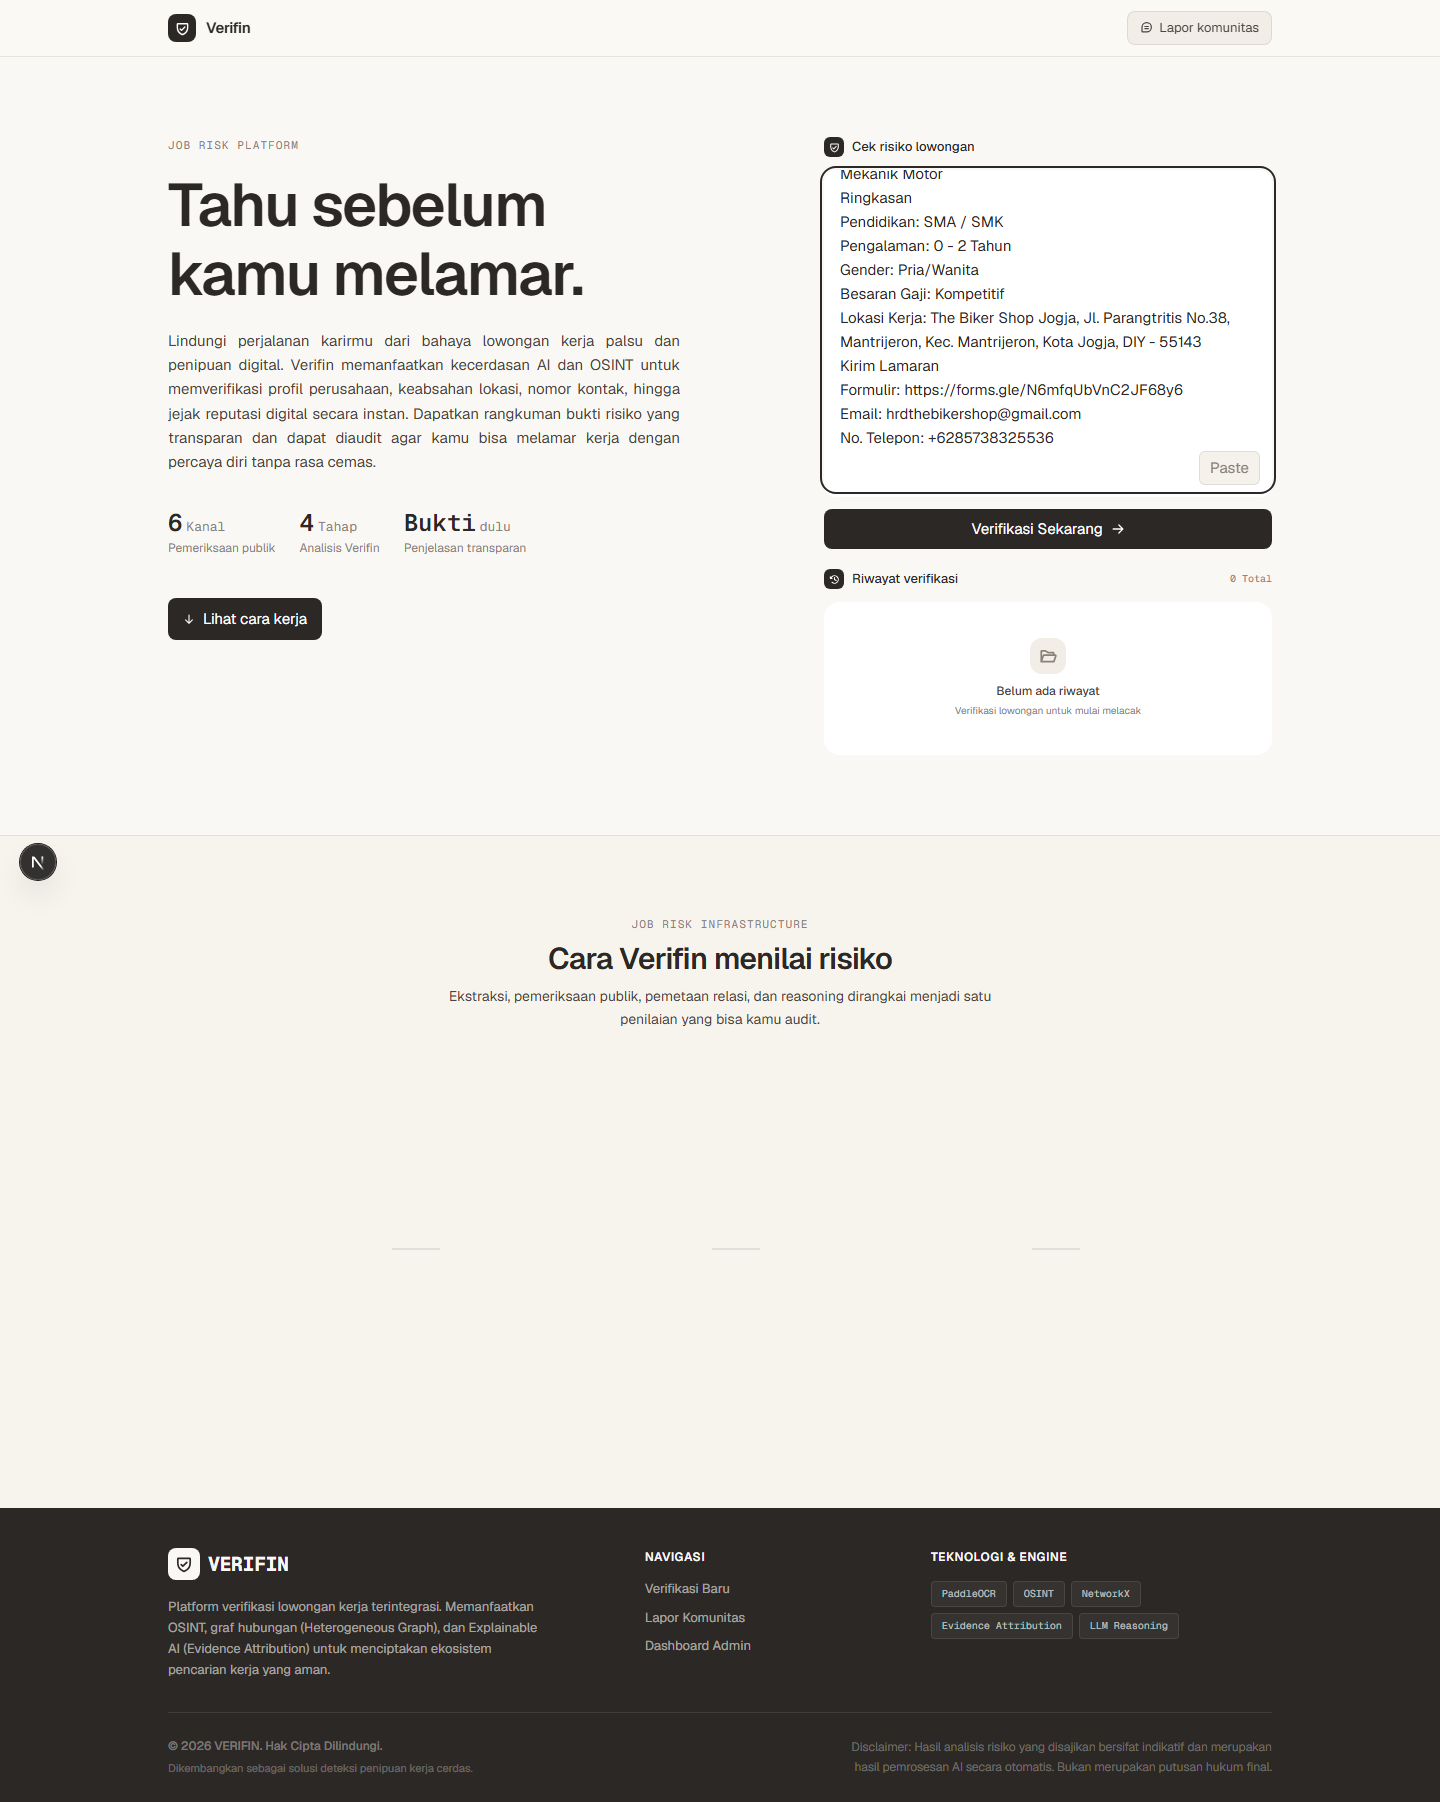
\includegraphics[width=\linewidth]{images/tes text.png}
    \label{fig:tes-text}
  \end{subfigure}\hfill
  \begin{subfigure}[t]{0.32\linewidth}
    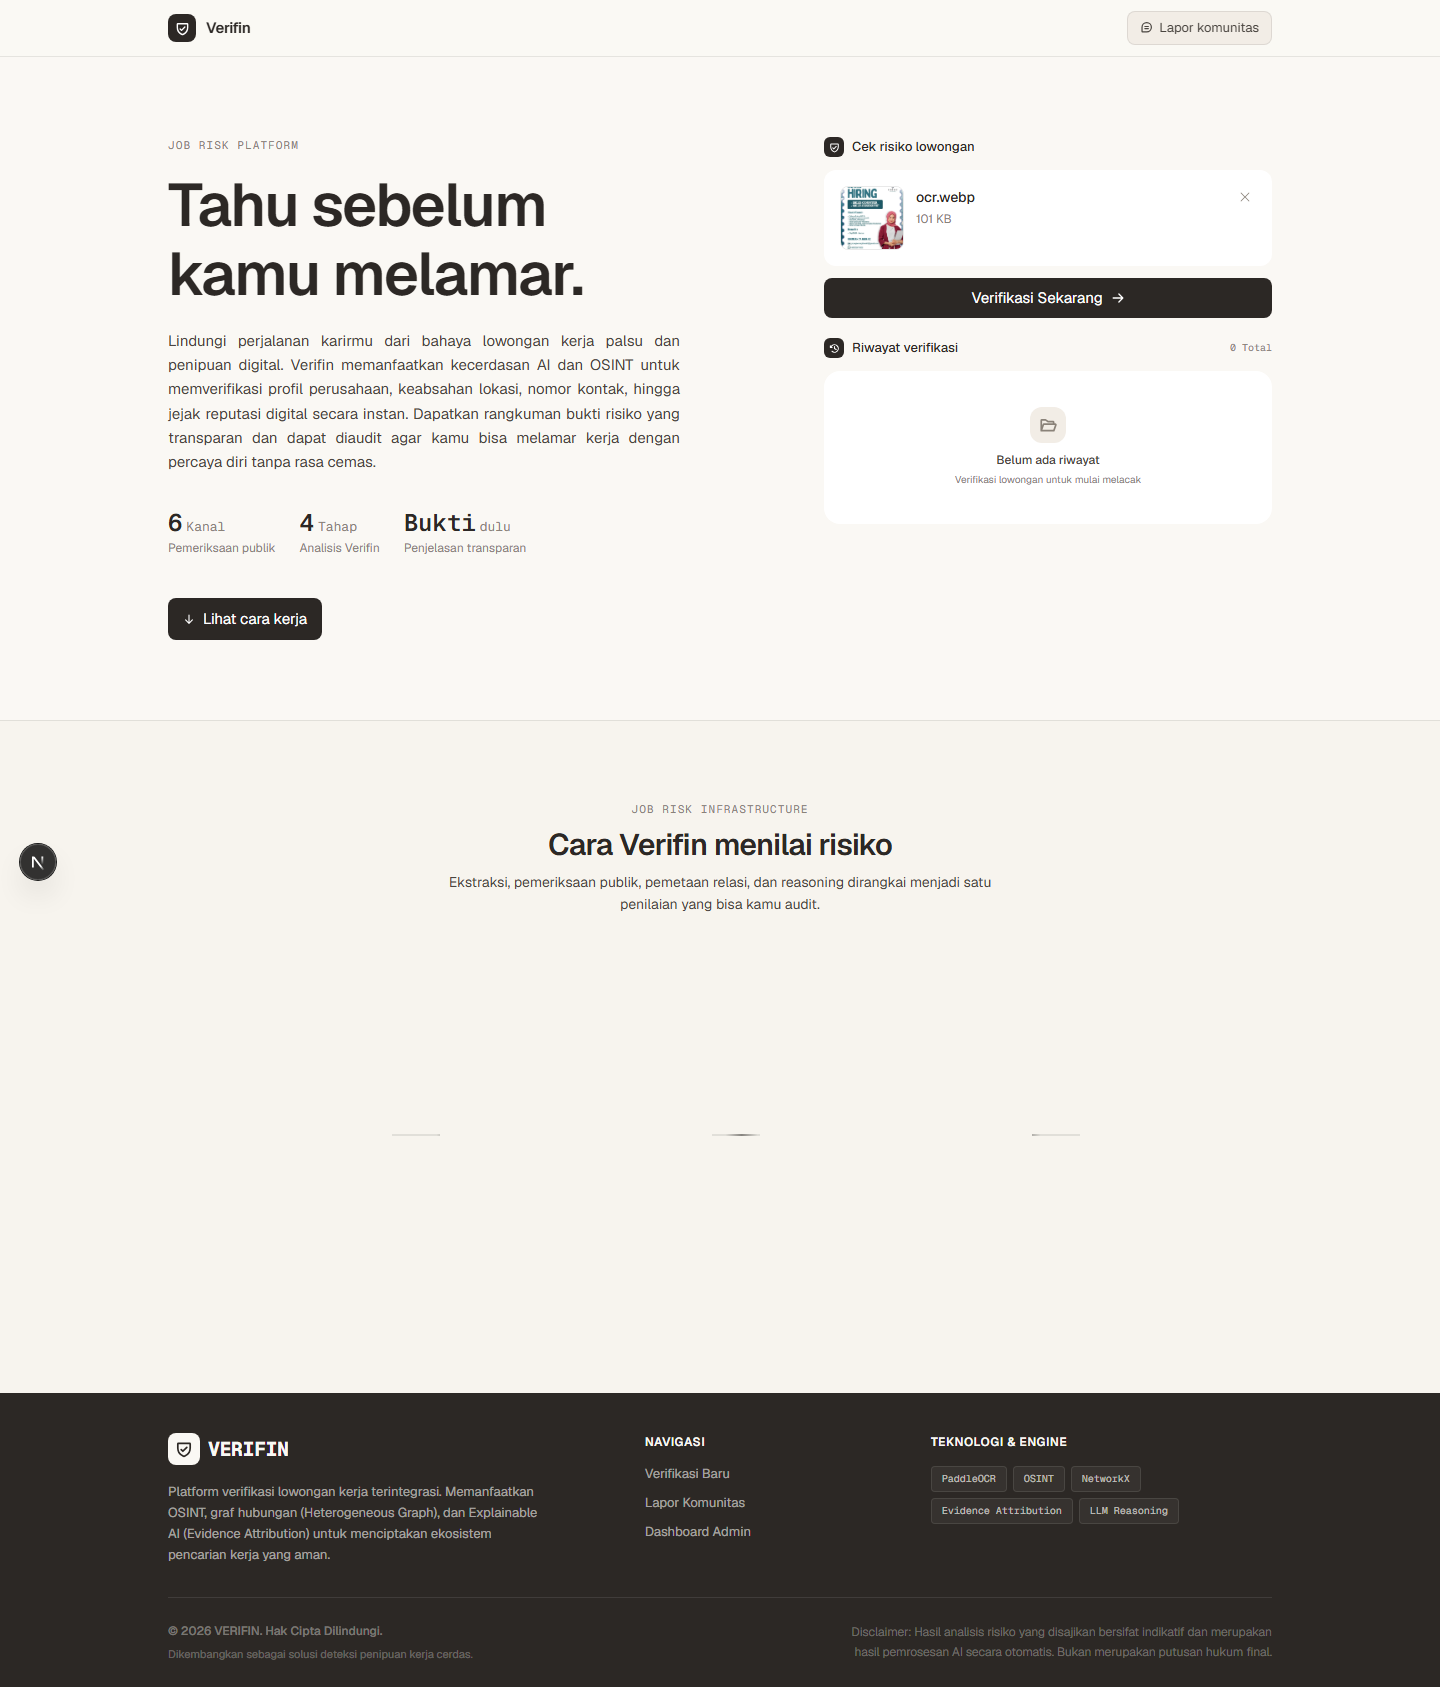
\includegraphics[width=\linewidth]{images/tes gambar.png}
    \label{fig:tes-gambar}
  \end{subfigure}\hfill
  \begin{subfigure}[t]{0.32\linewidth}
    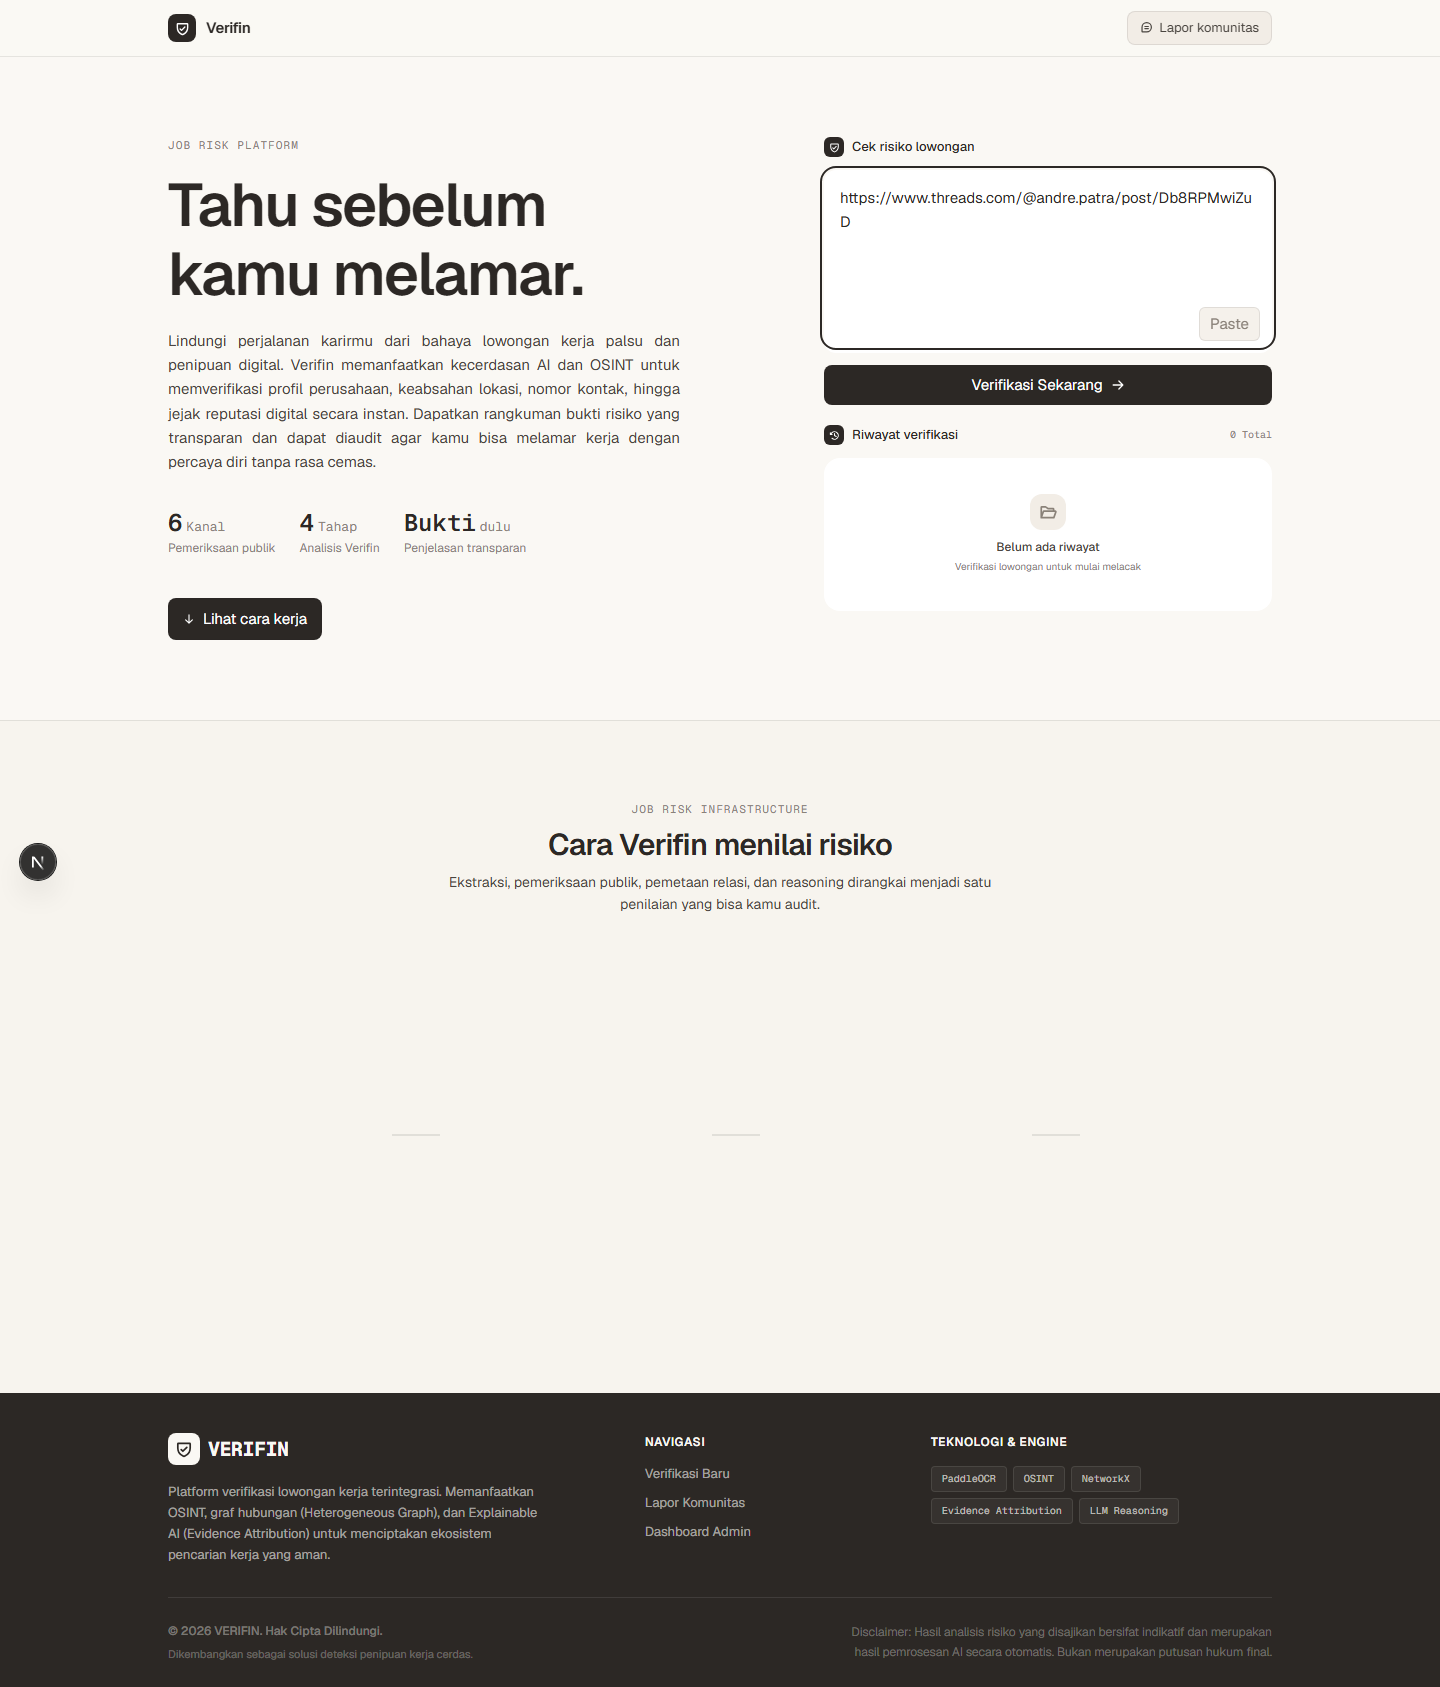
\includegraphics[width=\linewidth]{images/tes link.png}
    \label{fig:tes-link}
  \end{subfigure}
  \end{adjustwidth}
  \caption{Antarmuka Form Input Multi-Kanal Verifin}
  \label{fig:form-input}
\end{figure}

\subsection*{C.\quad Modal Progres Pemrosesan Pipeline Real-Time}
\addcontentsline{toc}{subsection}{C. Modal Progres Pemrosesan Pipeline Real-Time}

\begin{figure}[H]
  \centering
  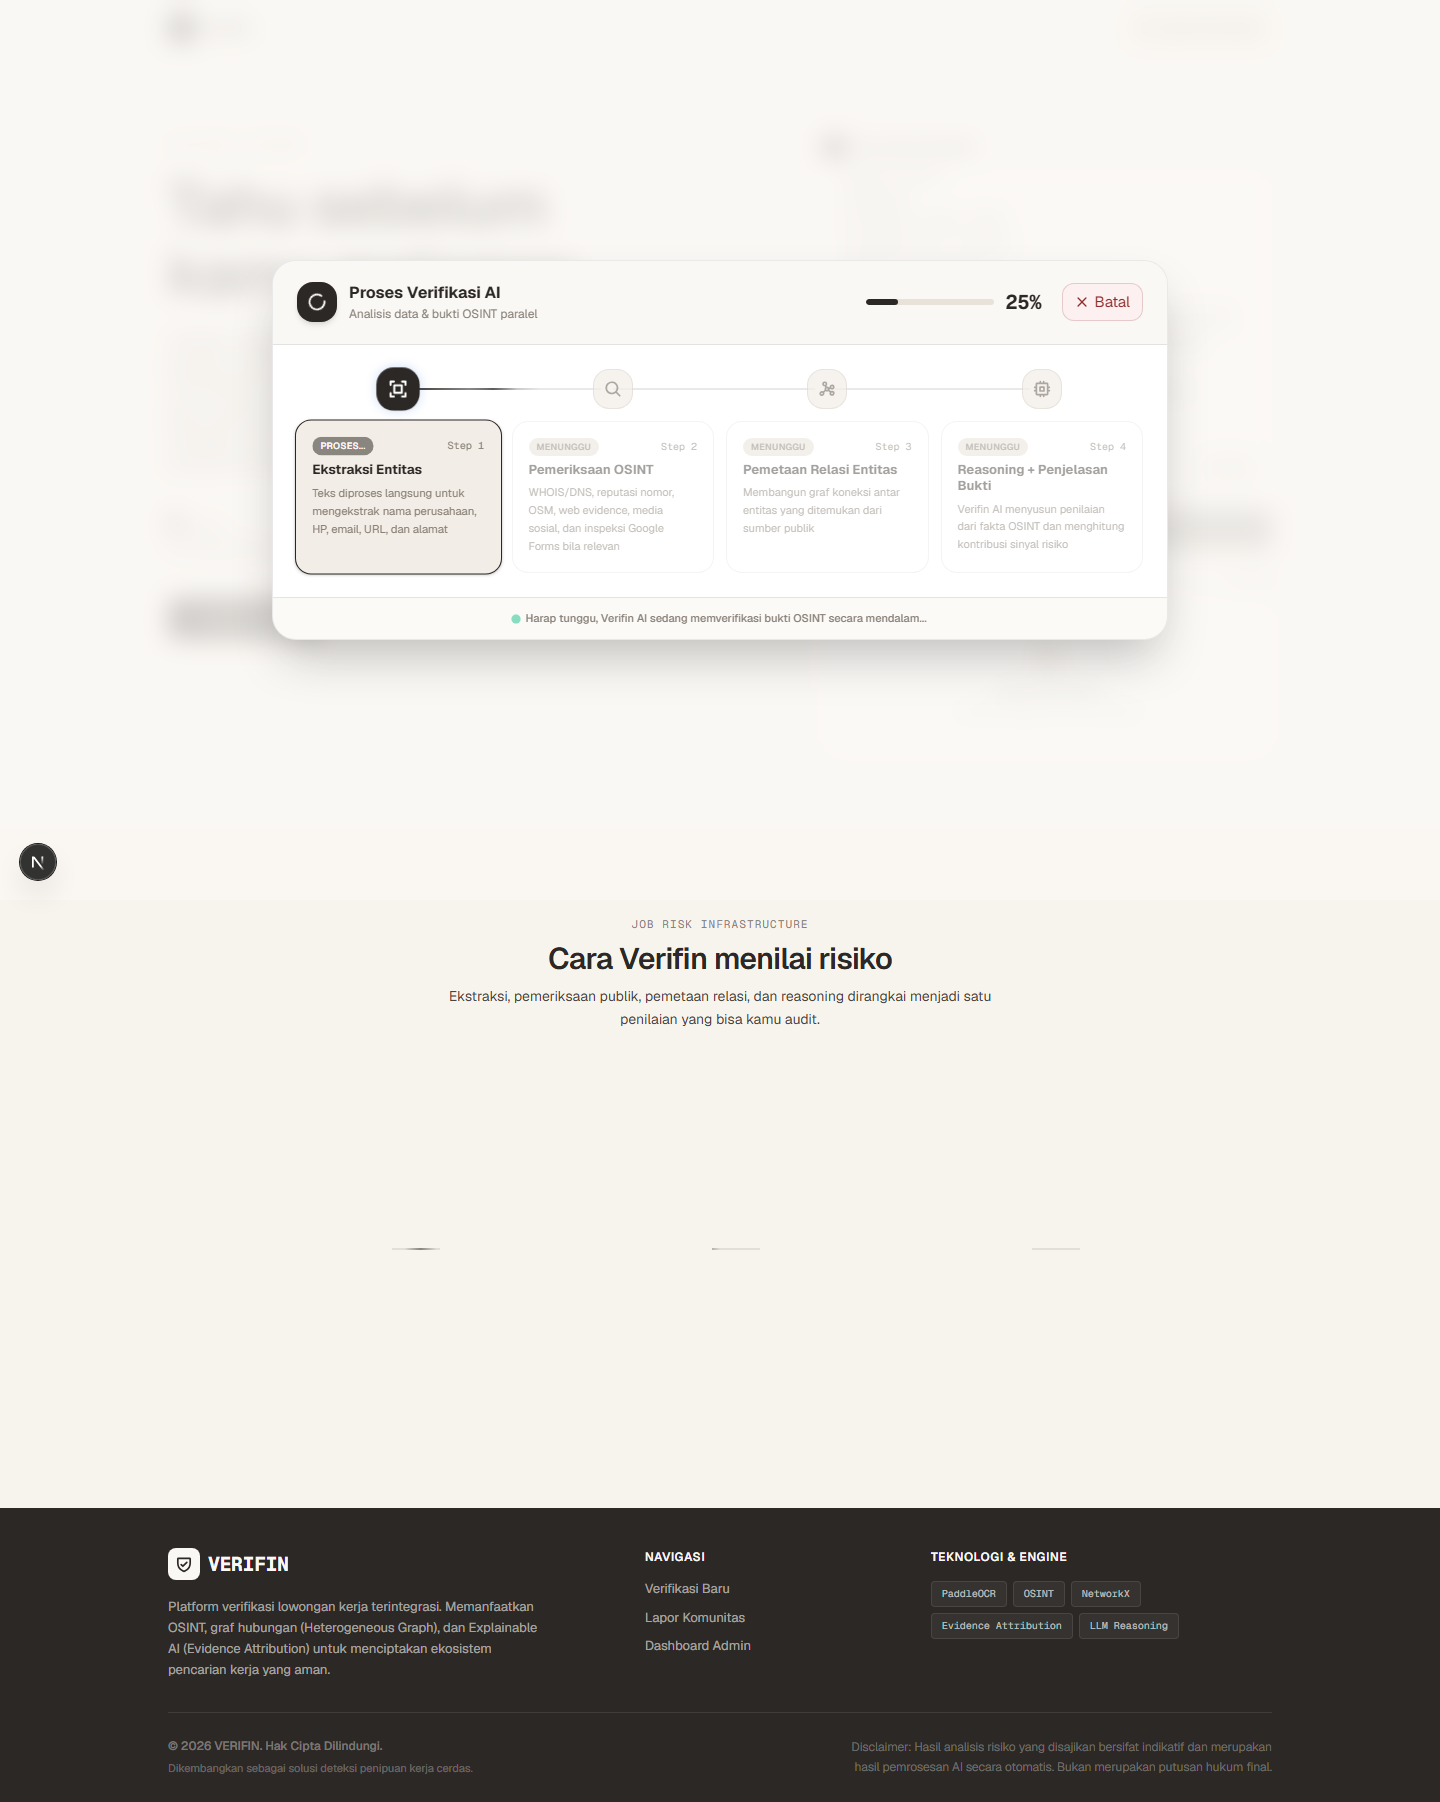
\includegraphics[width=0.55\linewidth]{images/mockup-loading.png}
  \caption{Modal Progres Pemrosesan Real-Time}
  \label{fig:mockup-loading}
\end{figure}

\subsection*{D.\quad Hasil Verifikasi \& Dashboard Analisis Per-Kanal}
\addcontentsline{toc}{subsection}{D. Hasil Verifikasi \& Dashboard Analisis Per-Kanal}

\subsubsection*{1.\quad Skenario Input Teks (Studi Kasus The Biker Shop)}
\addcontentsline{toc}{subsubsection}{1. Skenario Input Teks (Studi Kasus The Biker Shop)}

\begin{figure}[H]
  \centering
  \begin{subfigure}[t]{0.49\linewidth}
    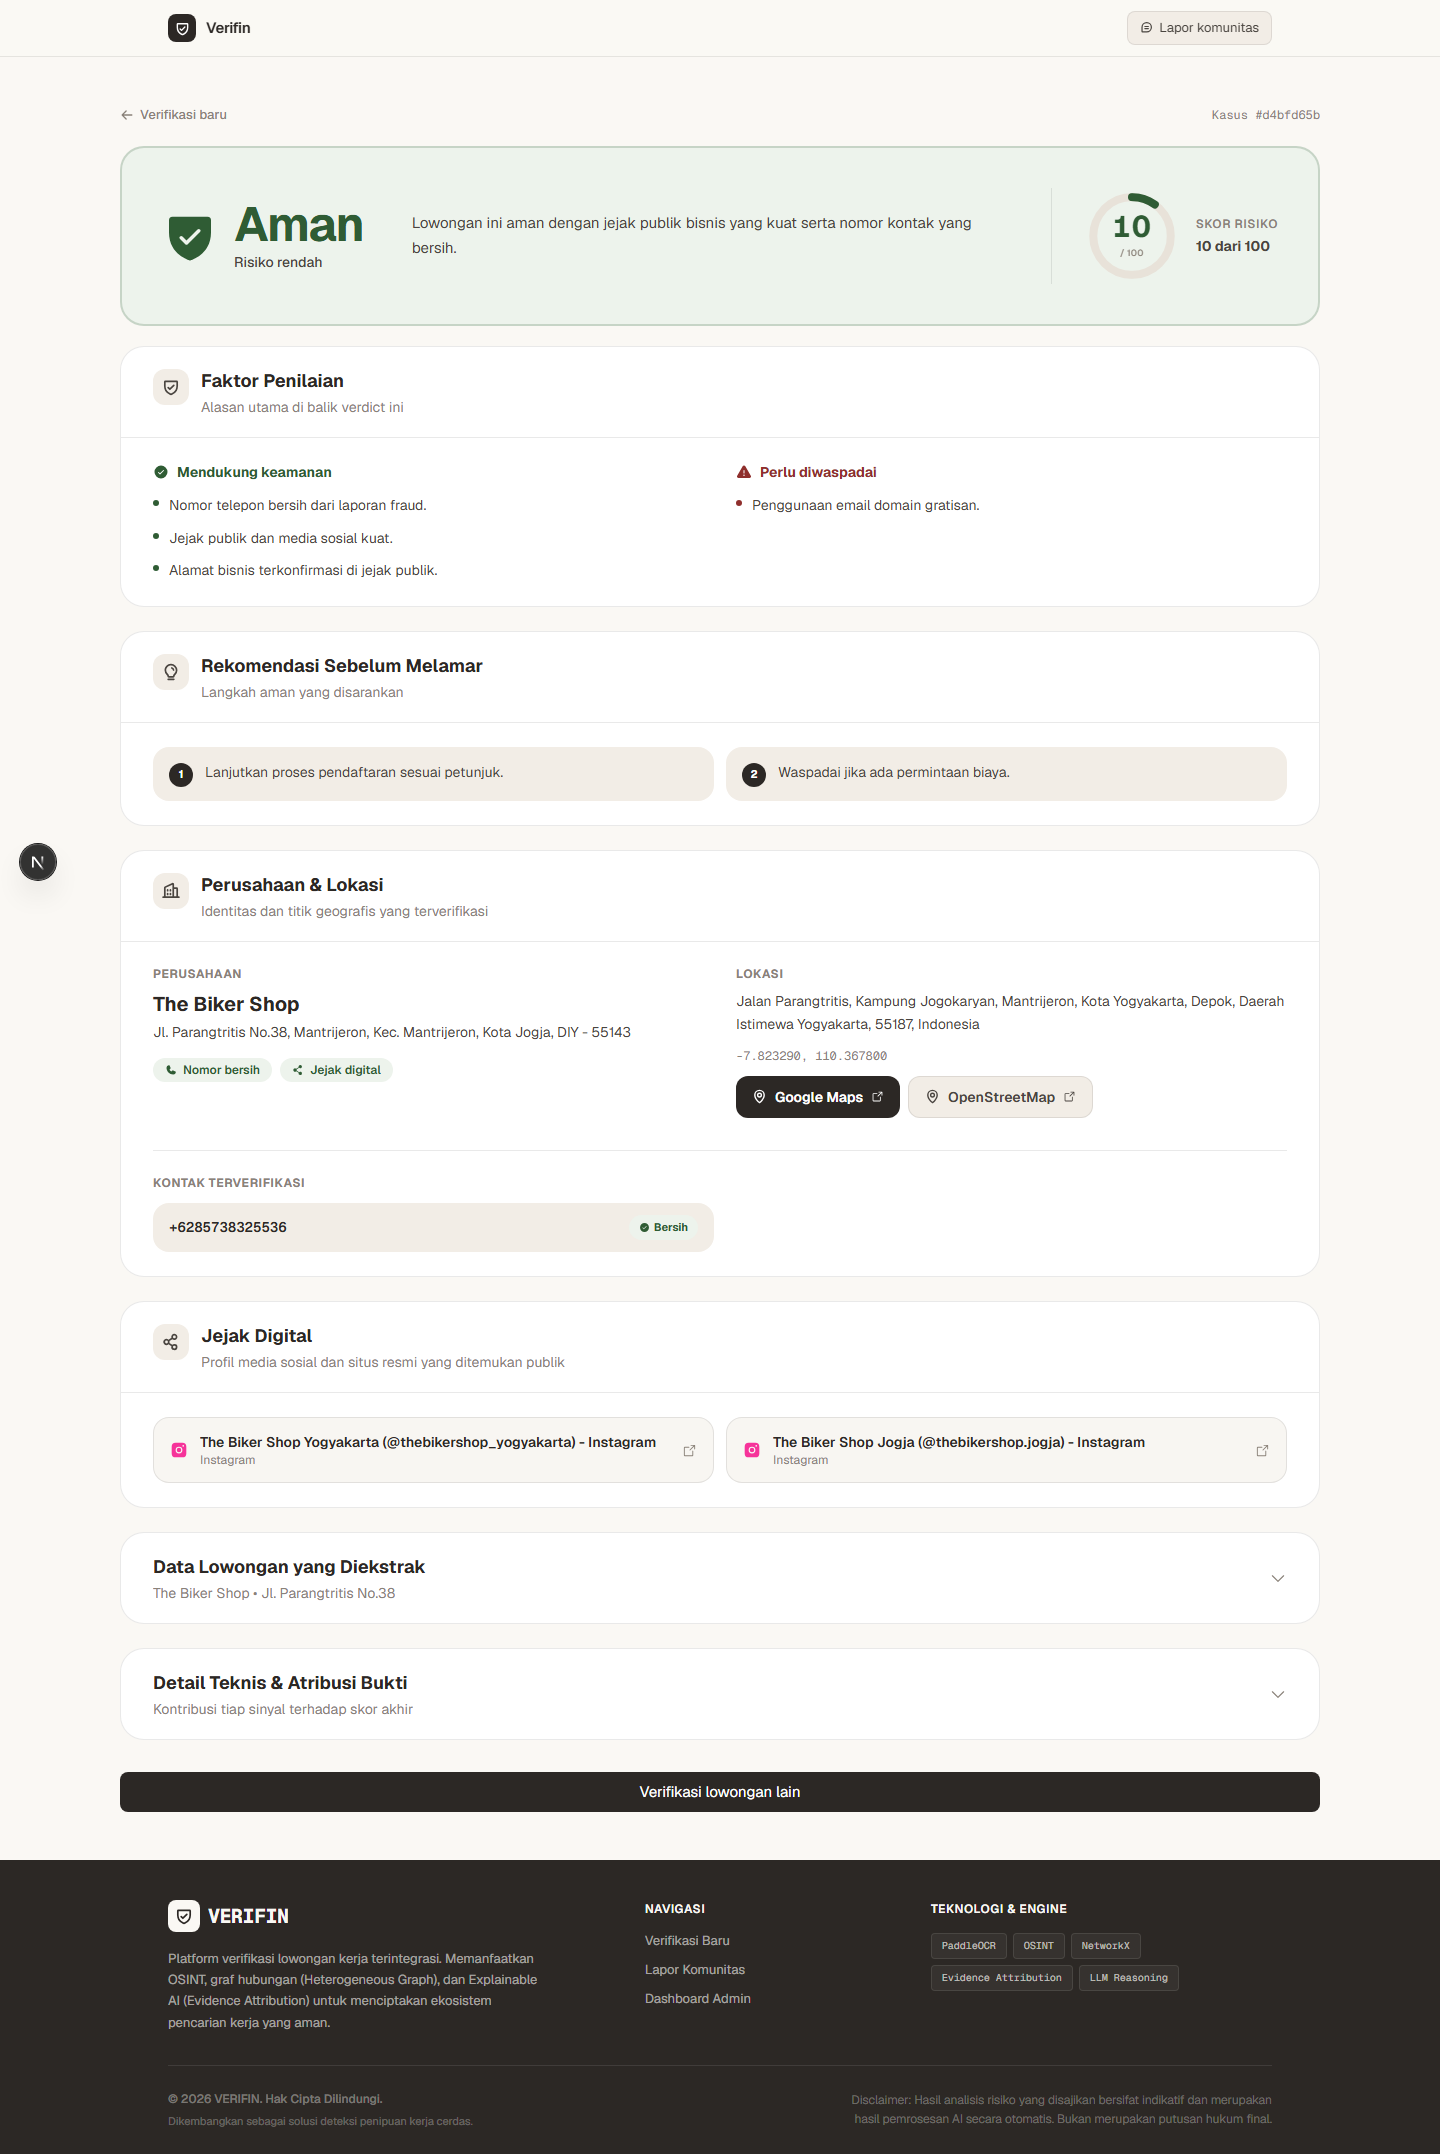
\includegraphics[width=\linewidth]{images/hasil text 1.png}
    \label{fig:hasil-text-1}
  \end{subfigure}\hfill
  \begin{subfigure}[t]{0.49\linewidth}
    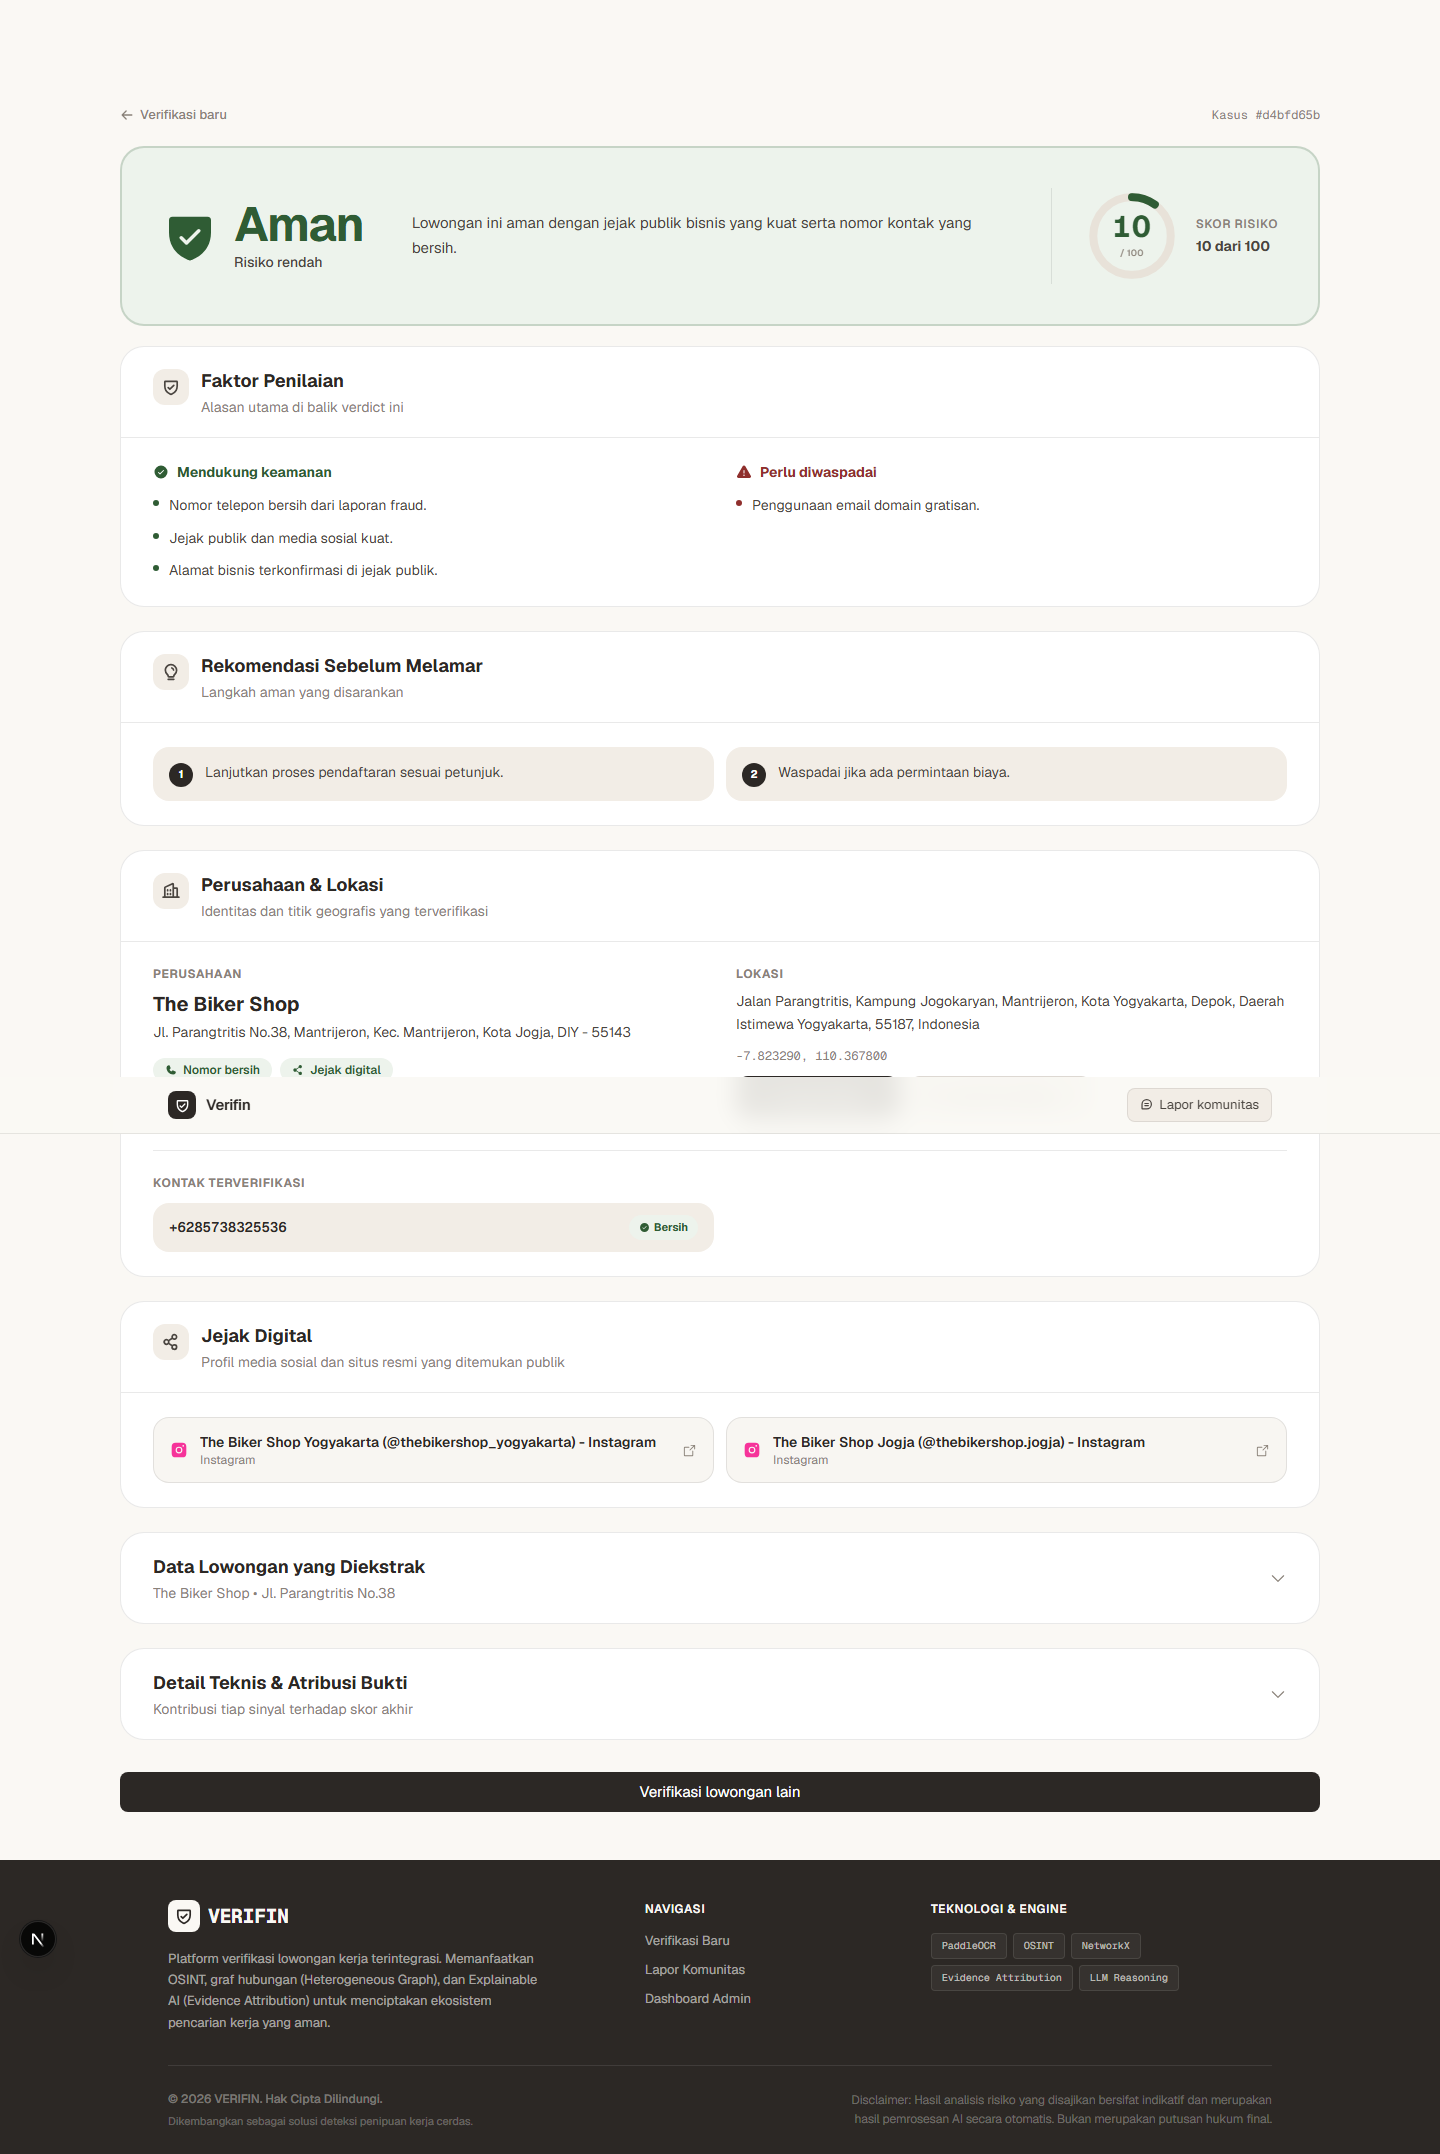
\includegraphics[width=\linewidth]{images/hasil text 2.png}
    \label{fig:hasil-text-2}
  \end{subfigure}
  \caption{Hasil Verifikasi Input Teks (Studi Kasus The Biker Shop)}
  \label{fig:hasil-text}
\end{figure}

\subsubsection*{2.\quad Skenario Input Gambar Poster / OCR (Studi Kasus VinFast Yogyakarta)}
\addcontentsline{toc}{subsubsection}{2. Skenario Input Gambar Poster / OCR (Studi Kasus VinFast Yogyakarta)}

\begin{figure}[H]
  \centering
  \begin{subfigure}[t]{0.49\linewidth}
    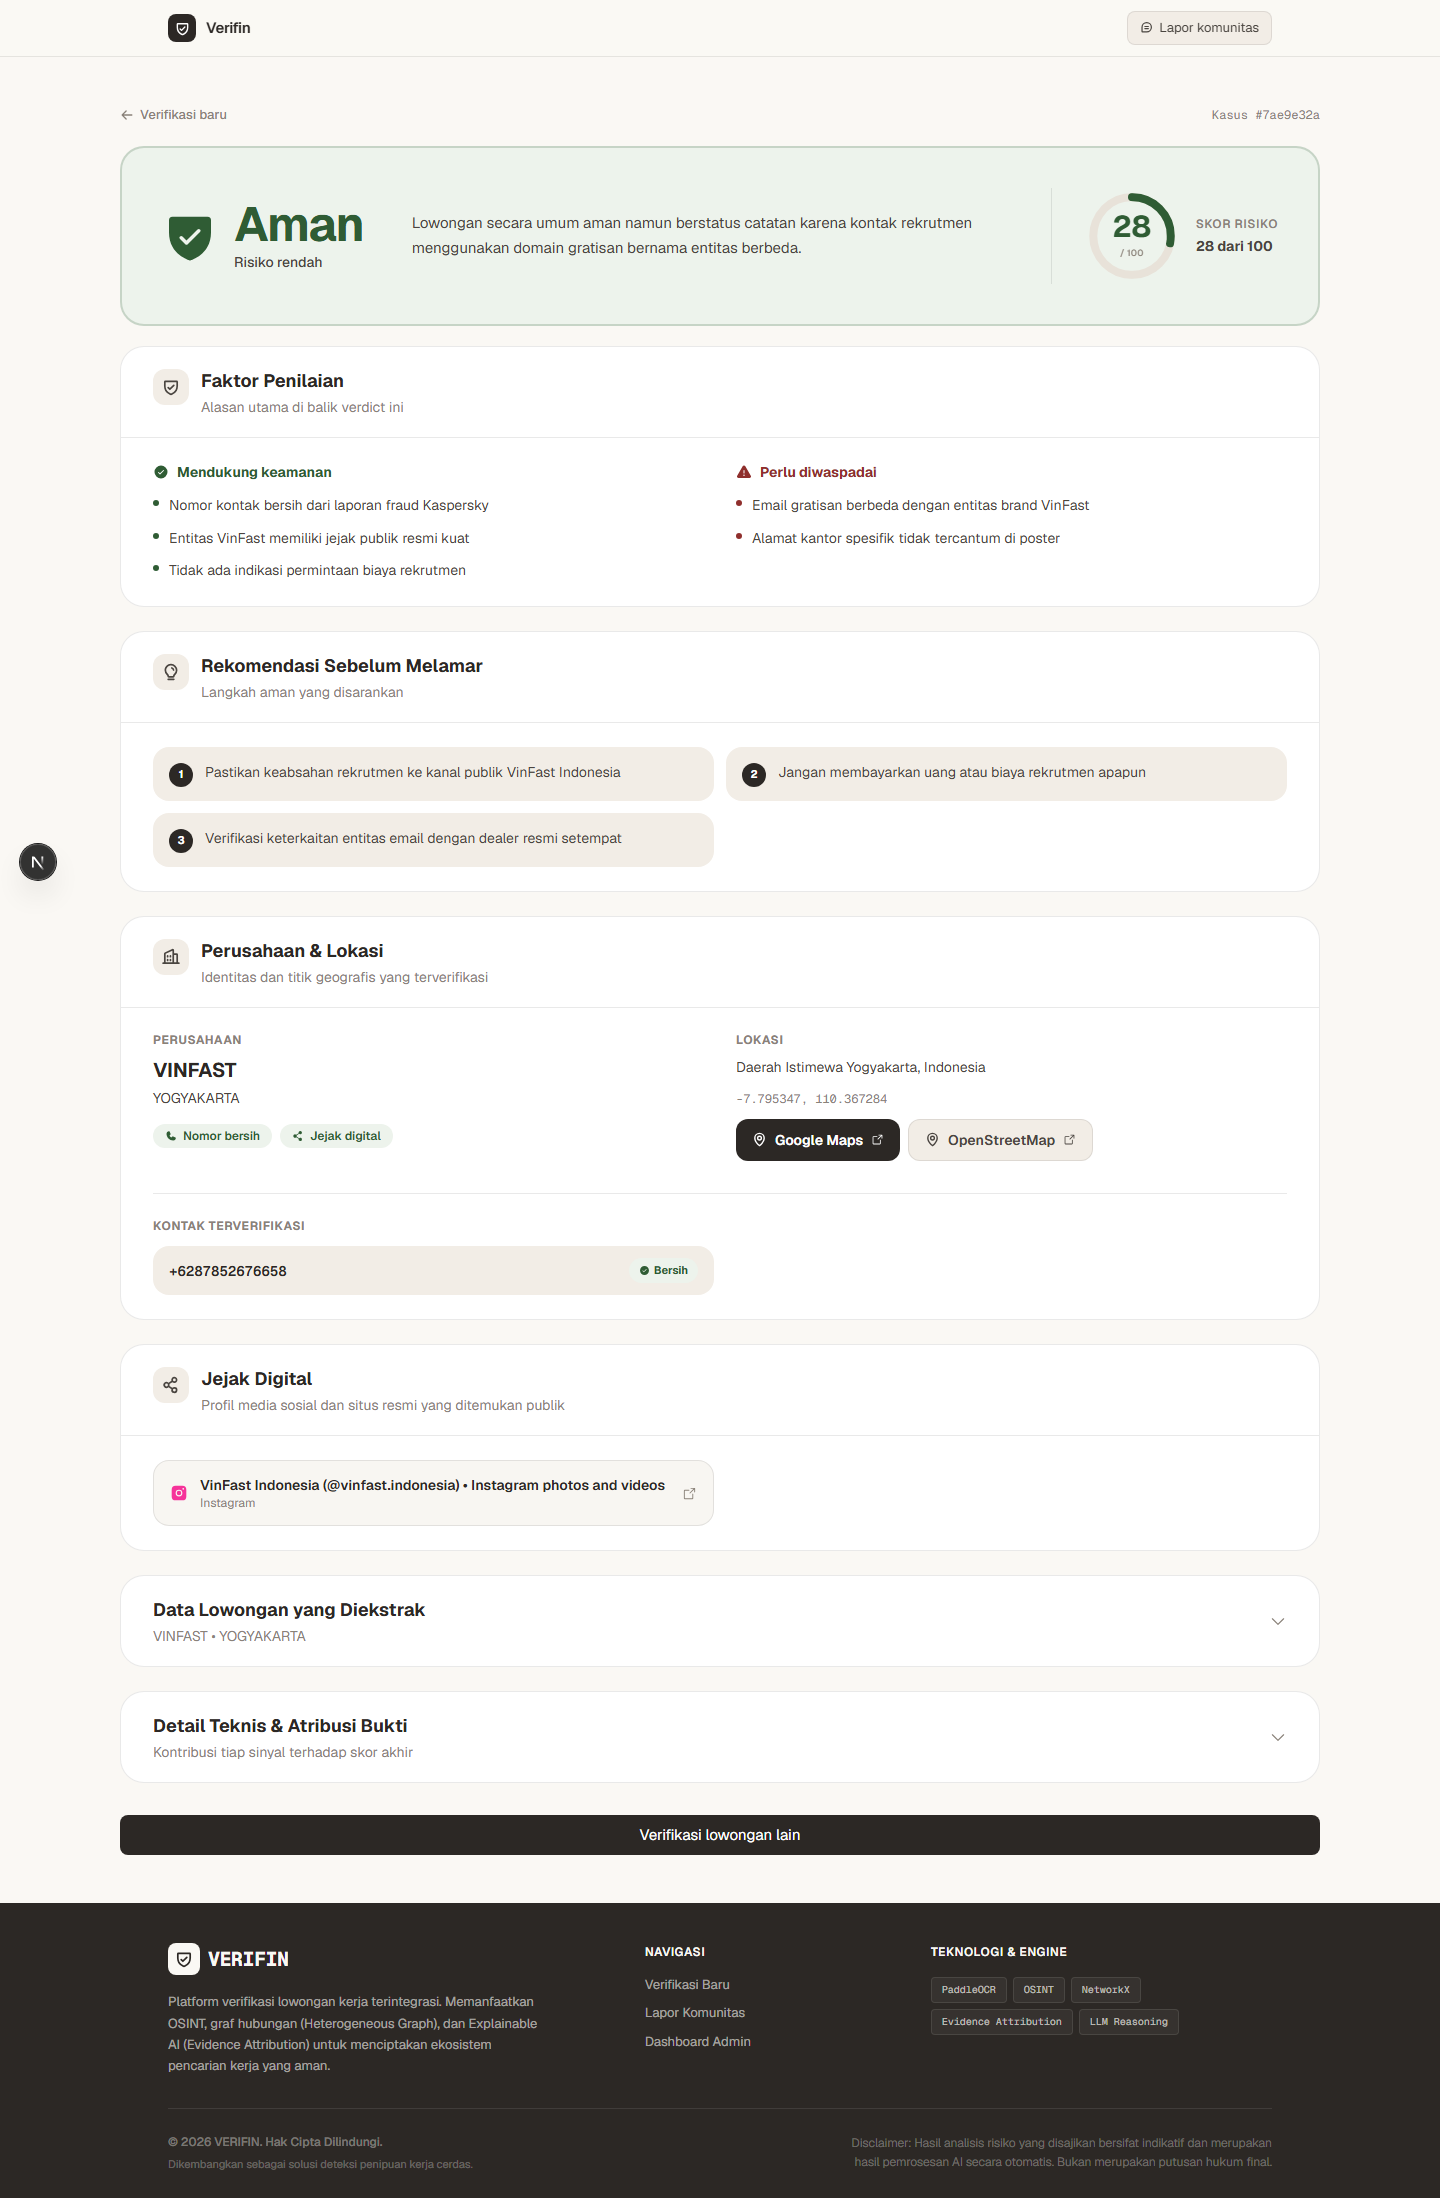
\includegraphics[width=\linewidth]{images/hasil gambar 1.png}
    \label{fig:hasil-gambar-1}
  \end{subfigure}\hfill
  \begin{subfigure}[t]{0.49\linewidth}
    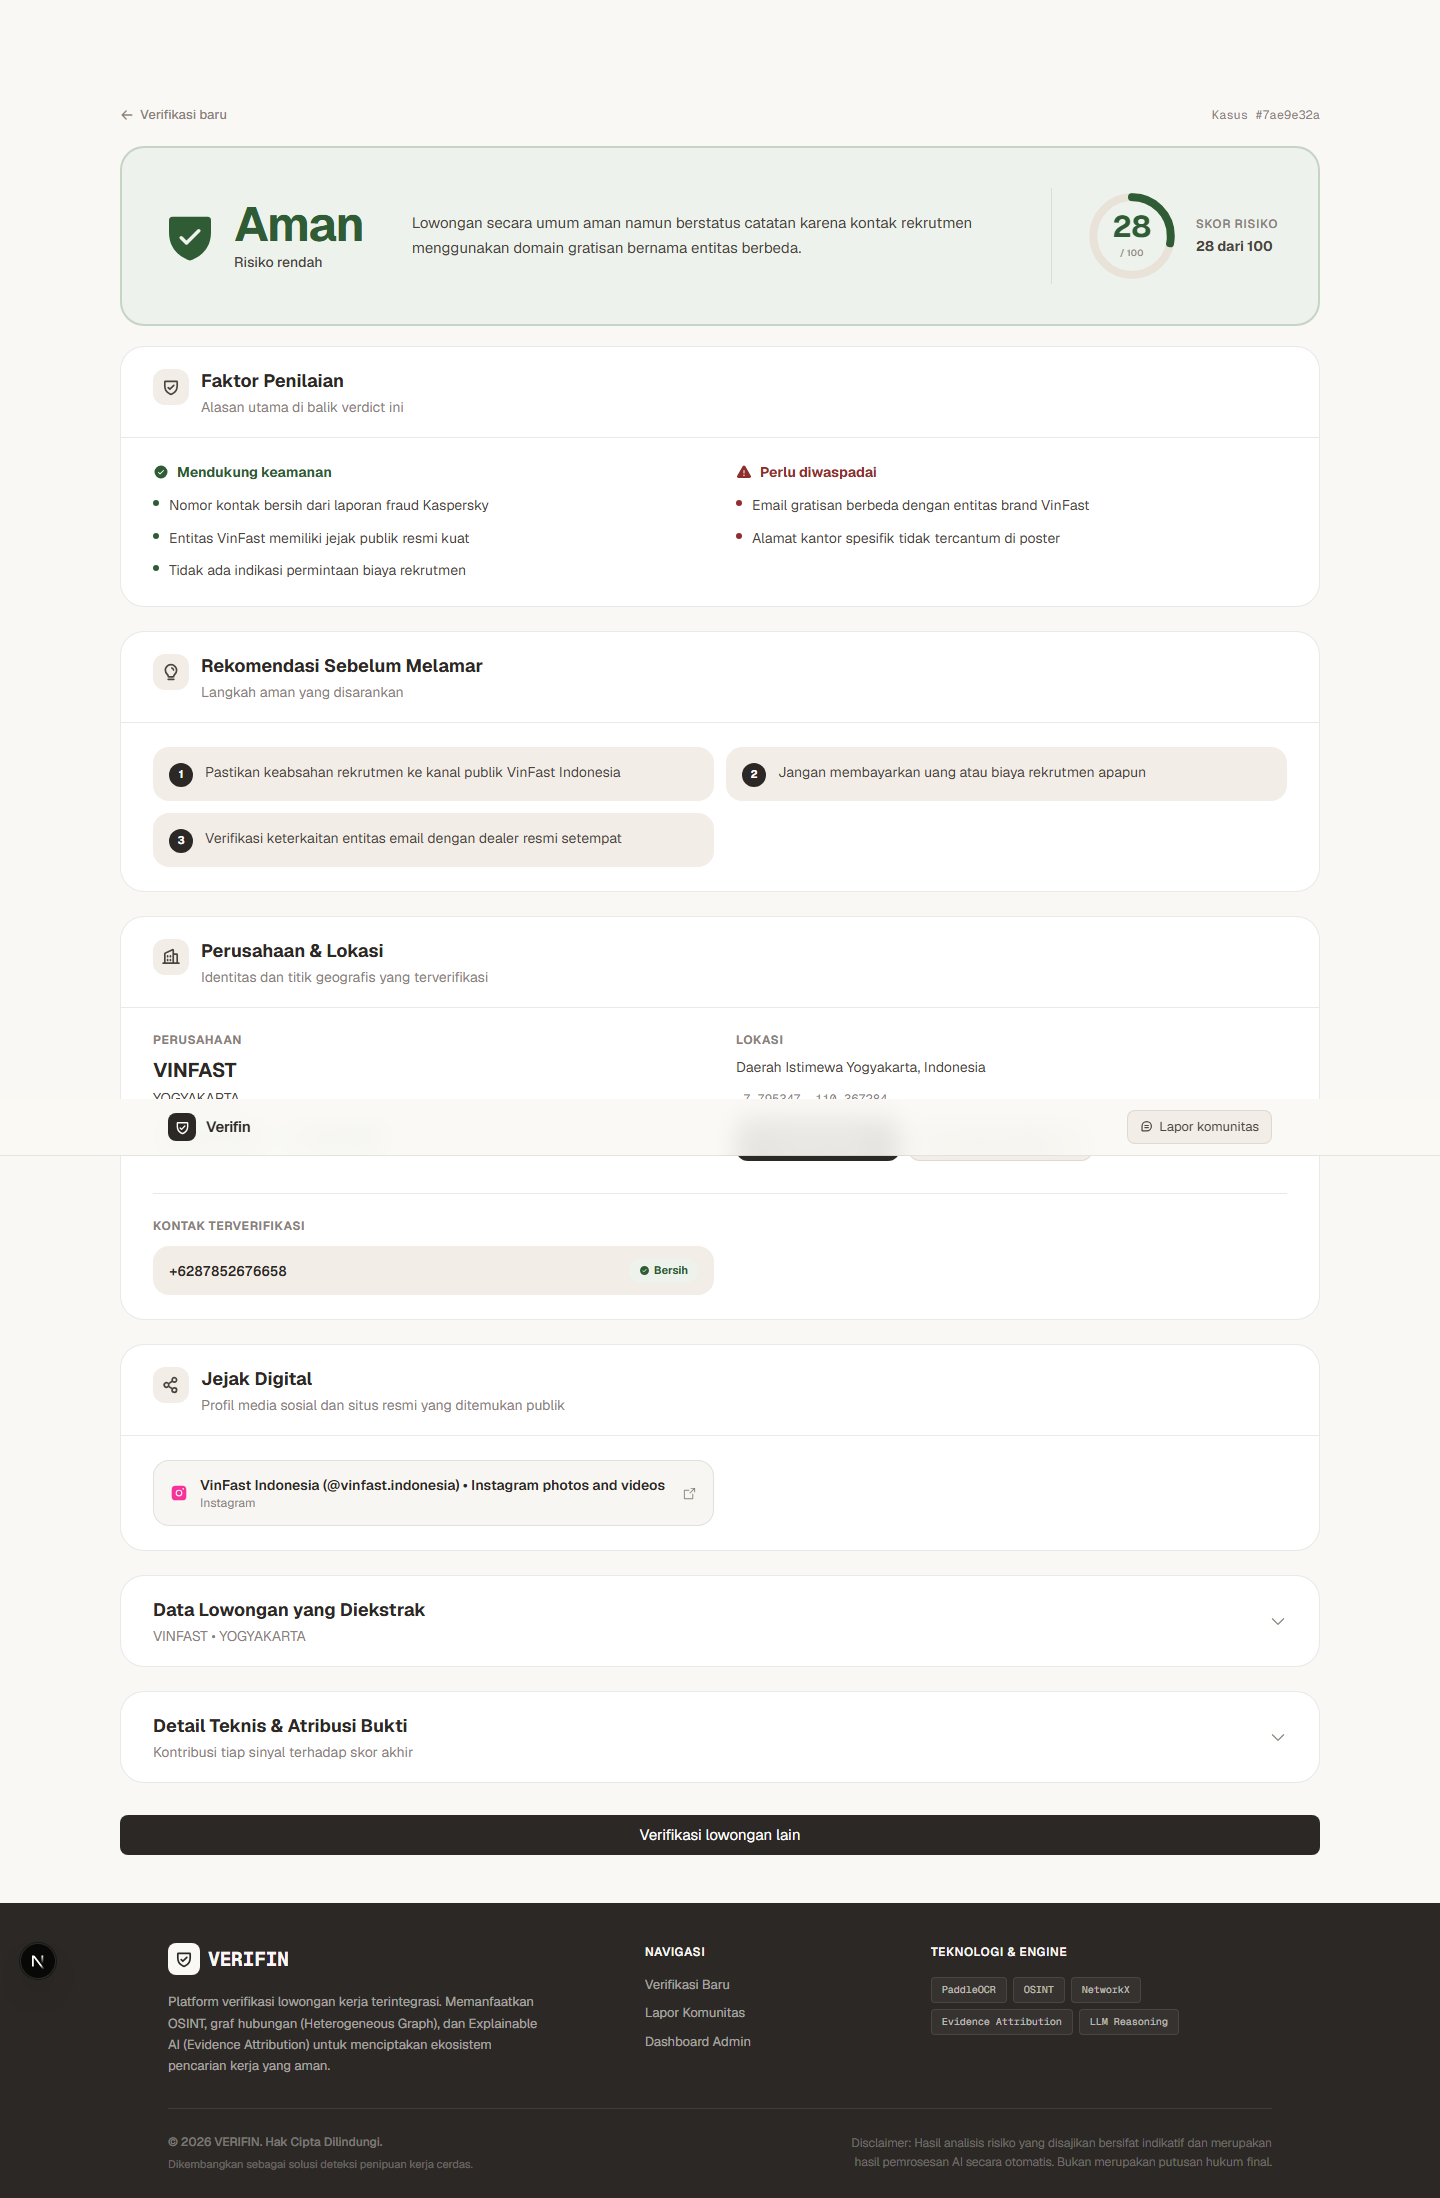
\includegraphics[width=\linewidth]{images/hasil gambar 2.png}
    \label{fig:hasil-gambar-2}
  \end{subfigure}
  \caption{Hasil Verifikasi Gambar Poster via OCR (Studi Kasus VinFast)}
  \label{fig:hasil-gambar}
\end{figure}

\subsubsection*{3.\quad Skenario Input Tautan / URL Web (Studi Kasus PT Sinergi Informatika Semen Indonesia)}
\addcontentsline{toc}{subsubsection}{3. Skenario Input Tautan / URL Web (Studi Kasus SISI)}

\begin{figure}[H]
  \centering
  \begin{subfigure}[t]{0.49\linewidth}
    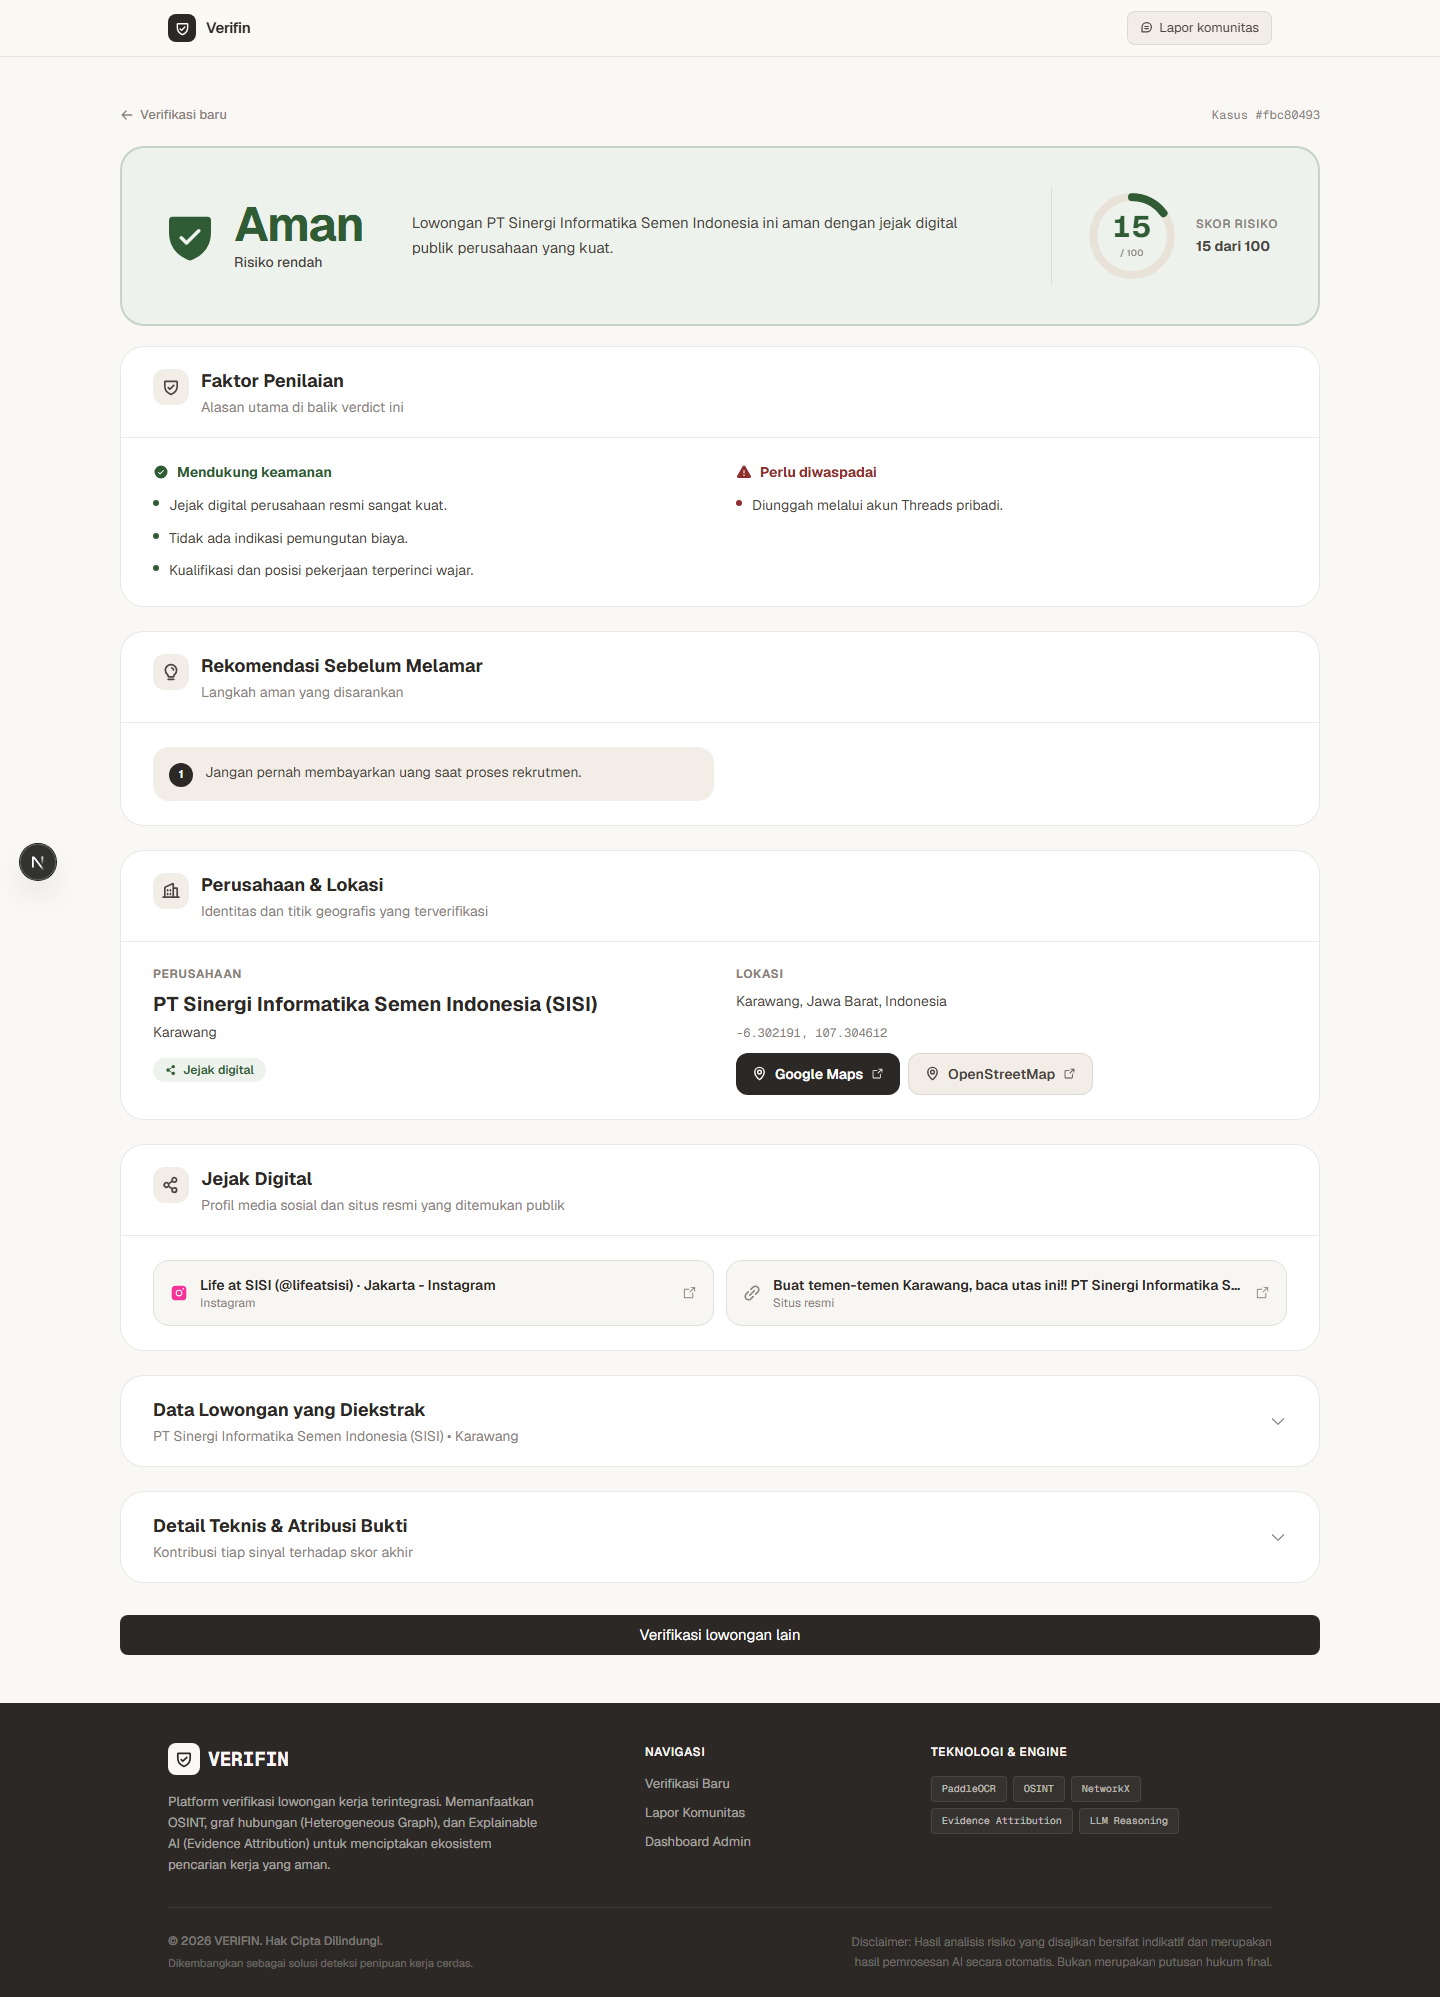
\includegraphics[width=\linewidth]{images/hasil link 1.png}
    \label{fig:hasil-link-1}
  \end{subfigure}\hfill
  \begin{subfigure}[t]{0.49\linewidth}
    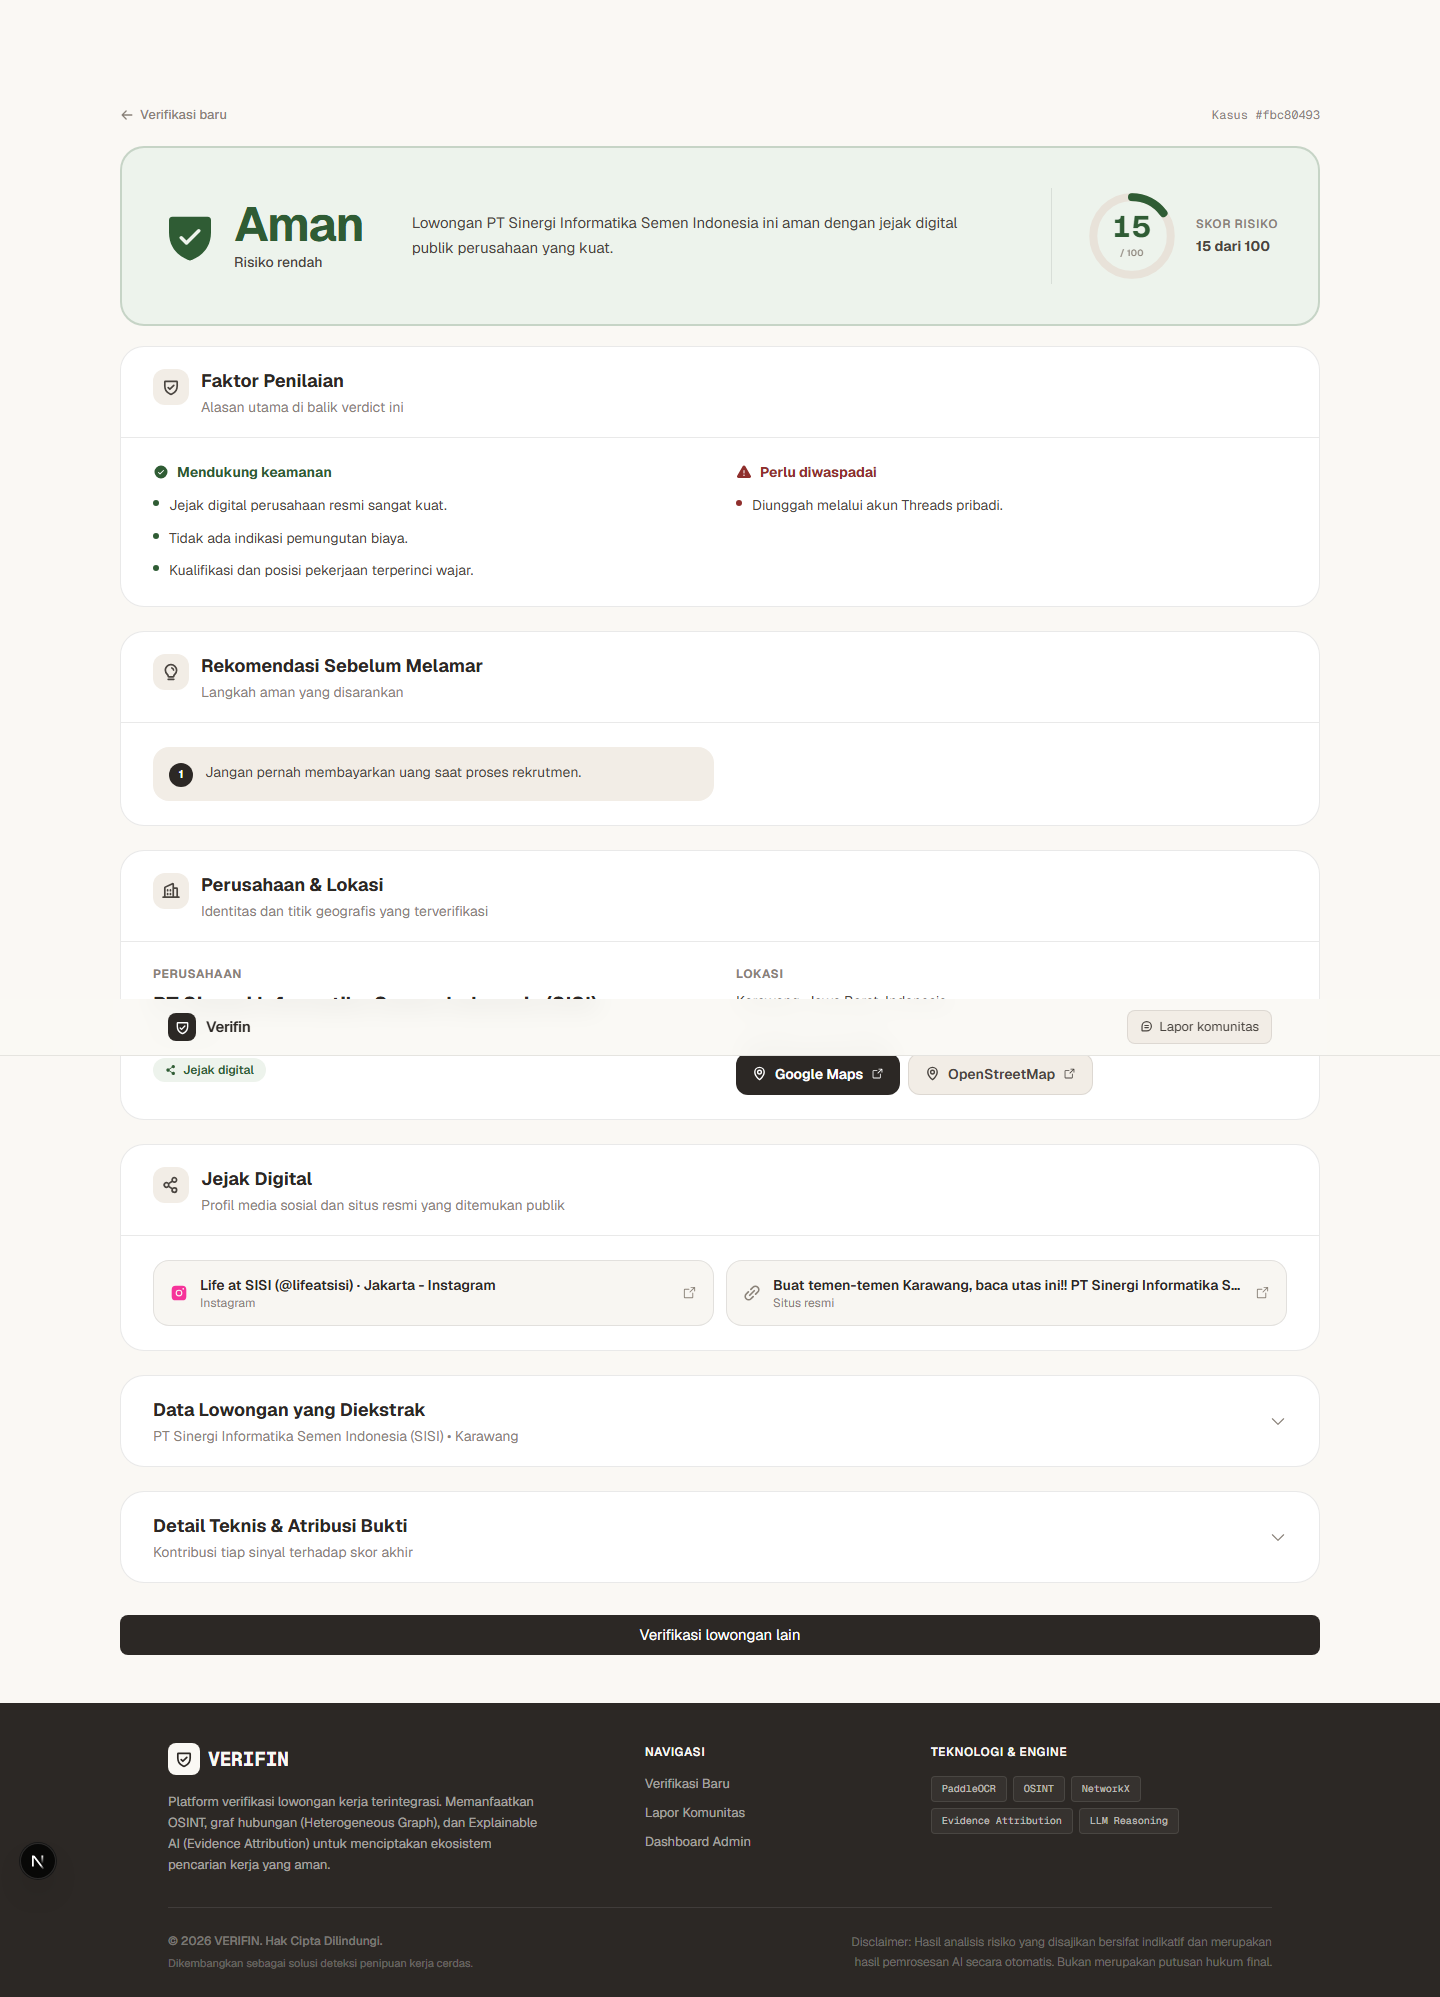
\includegraphics[width=\linewidth]{images/hasil link 2.png}
    \label{fig:hasil-link-2}
  \end{subfigure}
  \caption{Hasil Verifikasi Tautan URL (Studi Kasus PT SISI)}
  \label{fig:hasil-link}
\end{figure}

\subsection*{E.\quad Pengujian Kasus Negatif (Deteksi Lowongan Penipuan / Verdict BAHAYA)}
\addcontentsline{toc}{subsection}{E. Pengujian Kasus Negatif (Deteksi Lowongan Penipuan / Verdict BAHAYA)}

\begin{figure}[H]
  \centering
  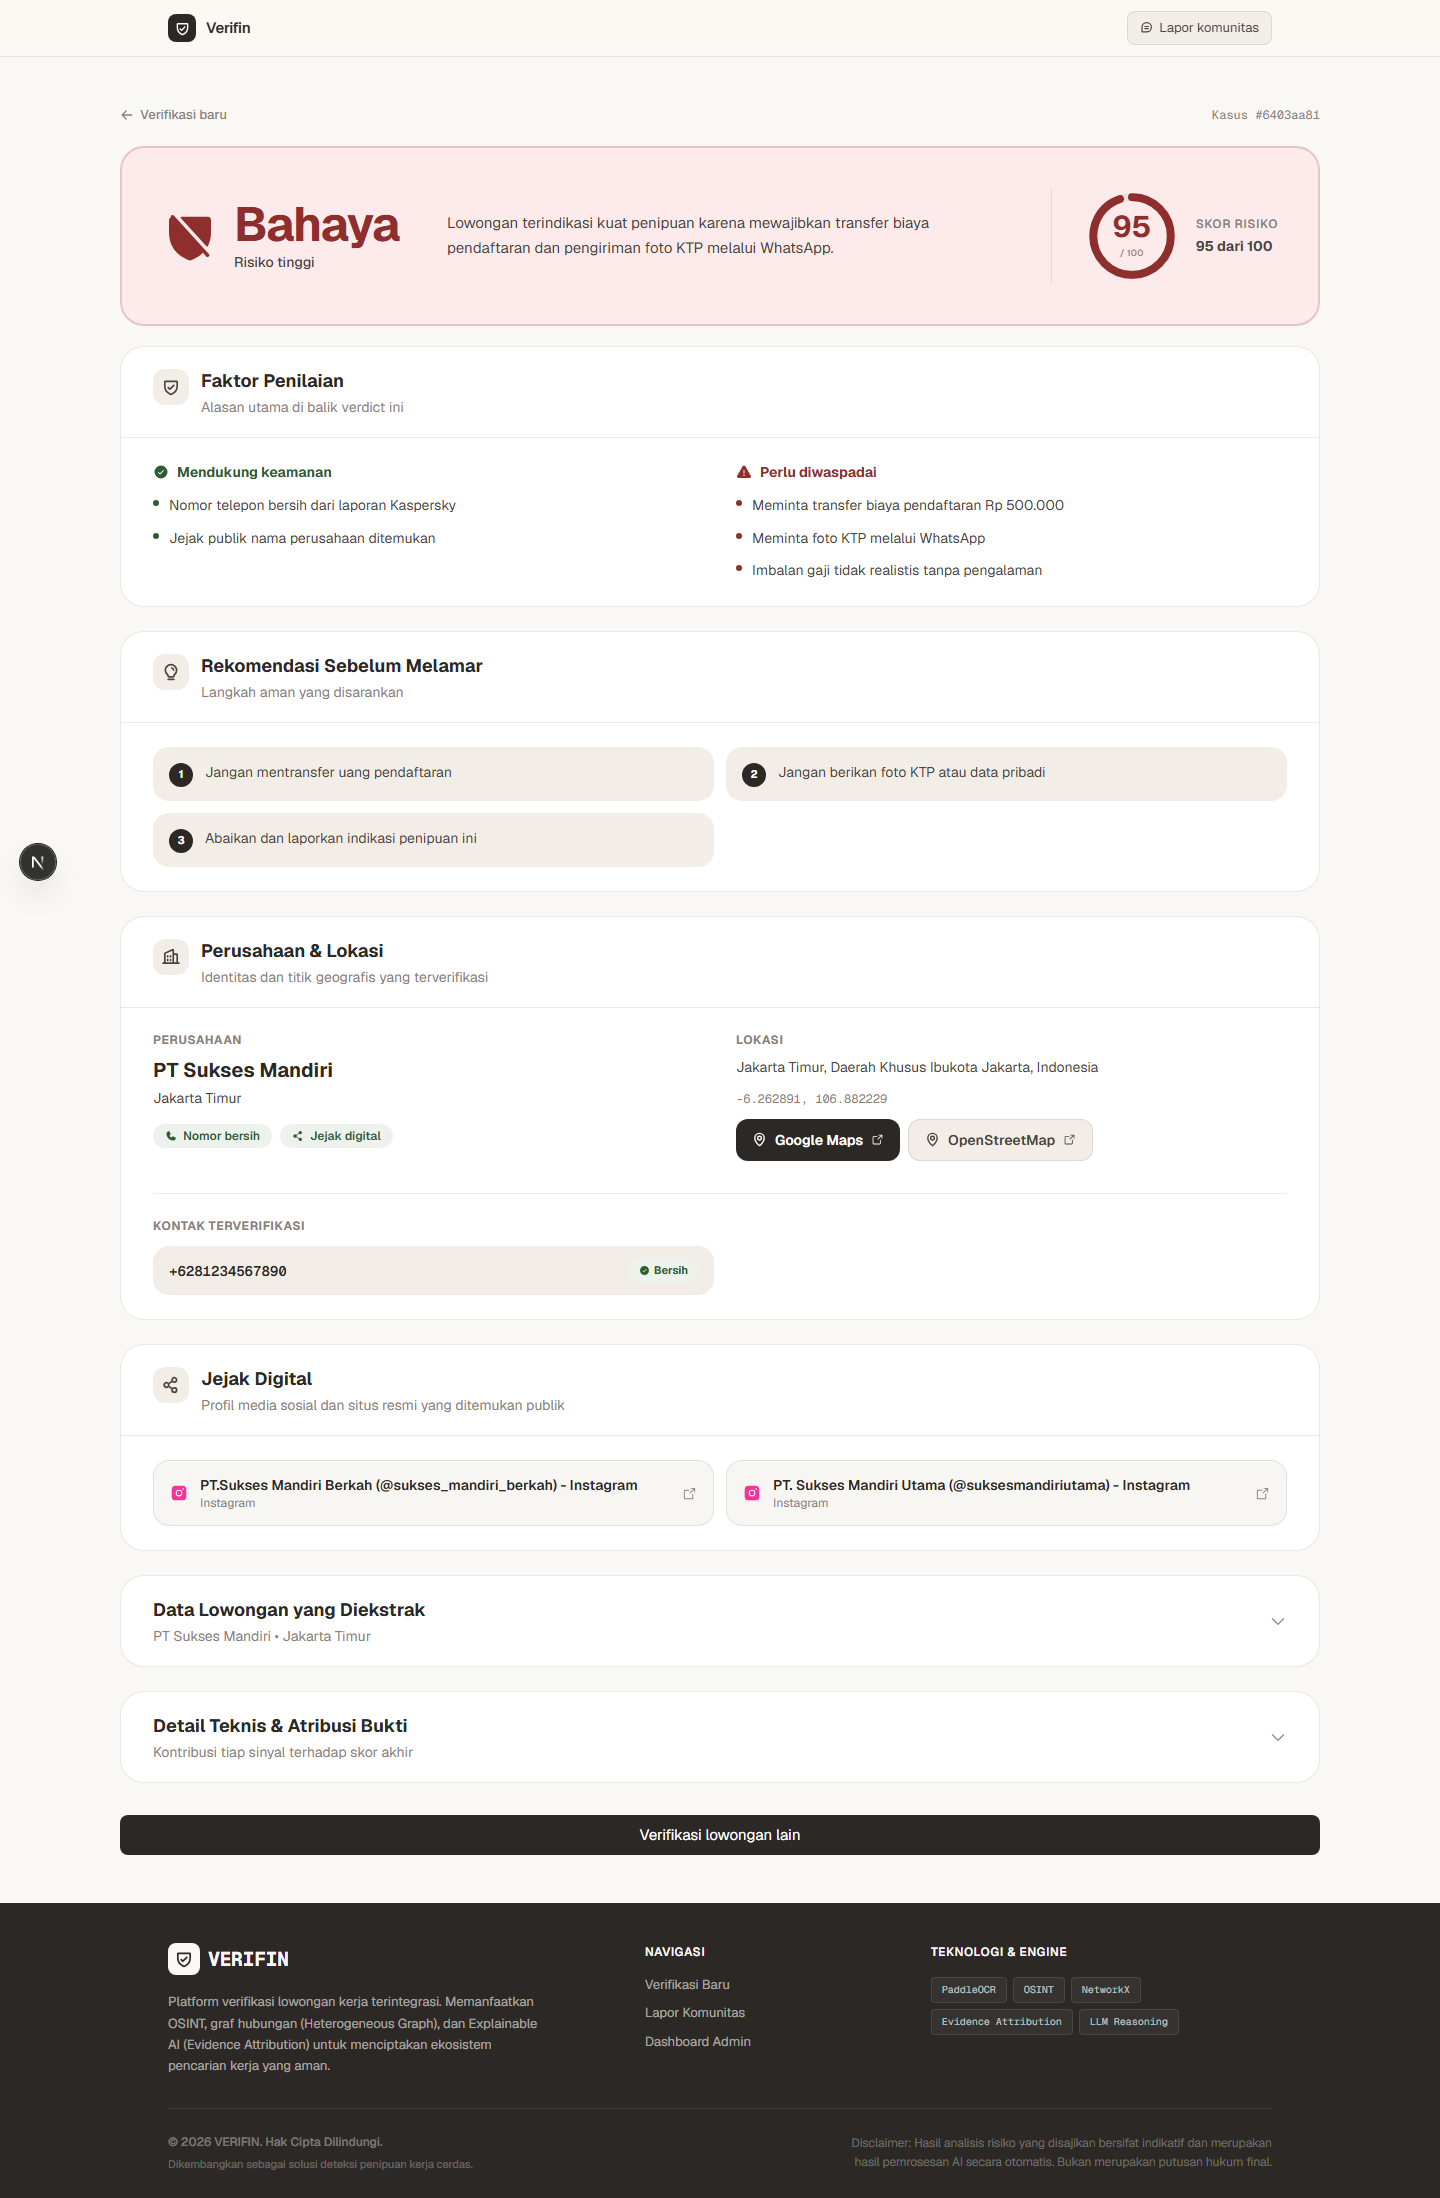
\includegraphics[width=0.55\linewidth]{images/hasil test negatif.png}
  \caption{Hasil Pengujian Kasus Negatif Penipuan (Verdict BAHAYA)}
  \label{fig:hasil-test-negatif}
\end{figure}

\subsection*{F.\quad Halaman Komunitas dan Riwayat Verifikasi}
\addcontentsline{toc}{subsection}{F. Halaman Komunitas dan Riwayat Verifikasi}

Selain alur verifikasi utama, Verifin menyediakan dua halaman pendukung yang memperkuat aspek
\textit{community monitoring} dan keberlanjutan penggunaan.

\begin{figure}[H]
  \centering
  \begin{subfigure}[t]{0.49\linewidth}
    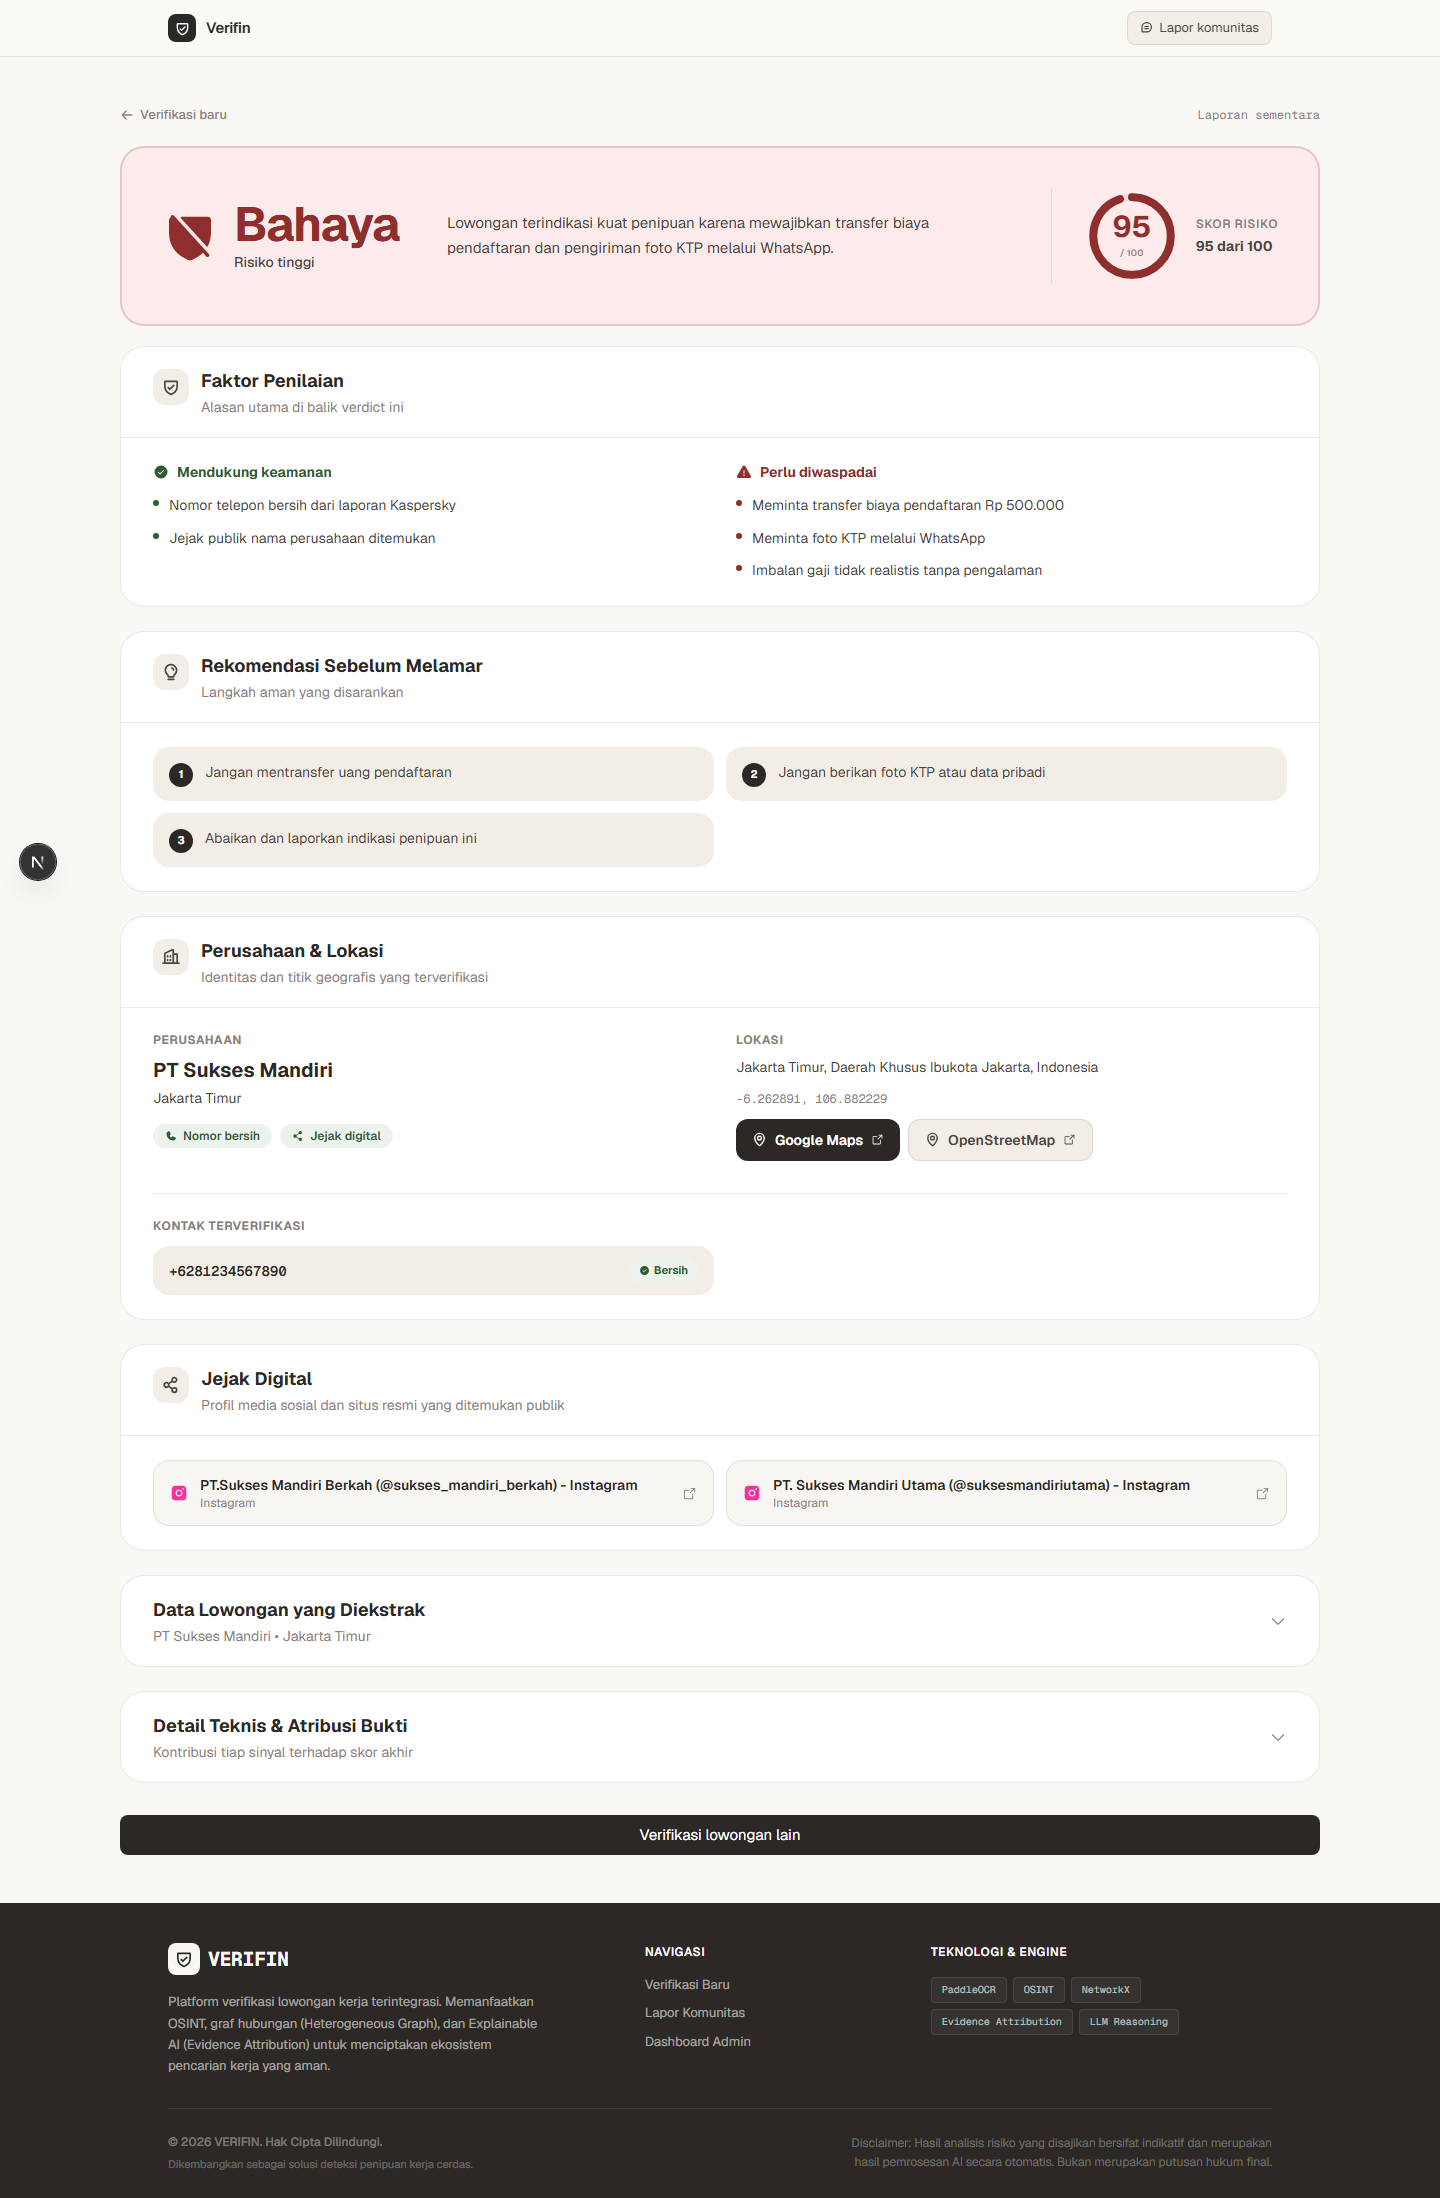
\includegraphics[width=\linewidth]{images/mockup-community.png}
    \label{fig:mockup-community}
  \end{subfigure}\hfill
  \begin{subfigure}[t]{0.49\linewidth}
    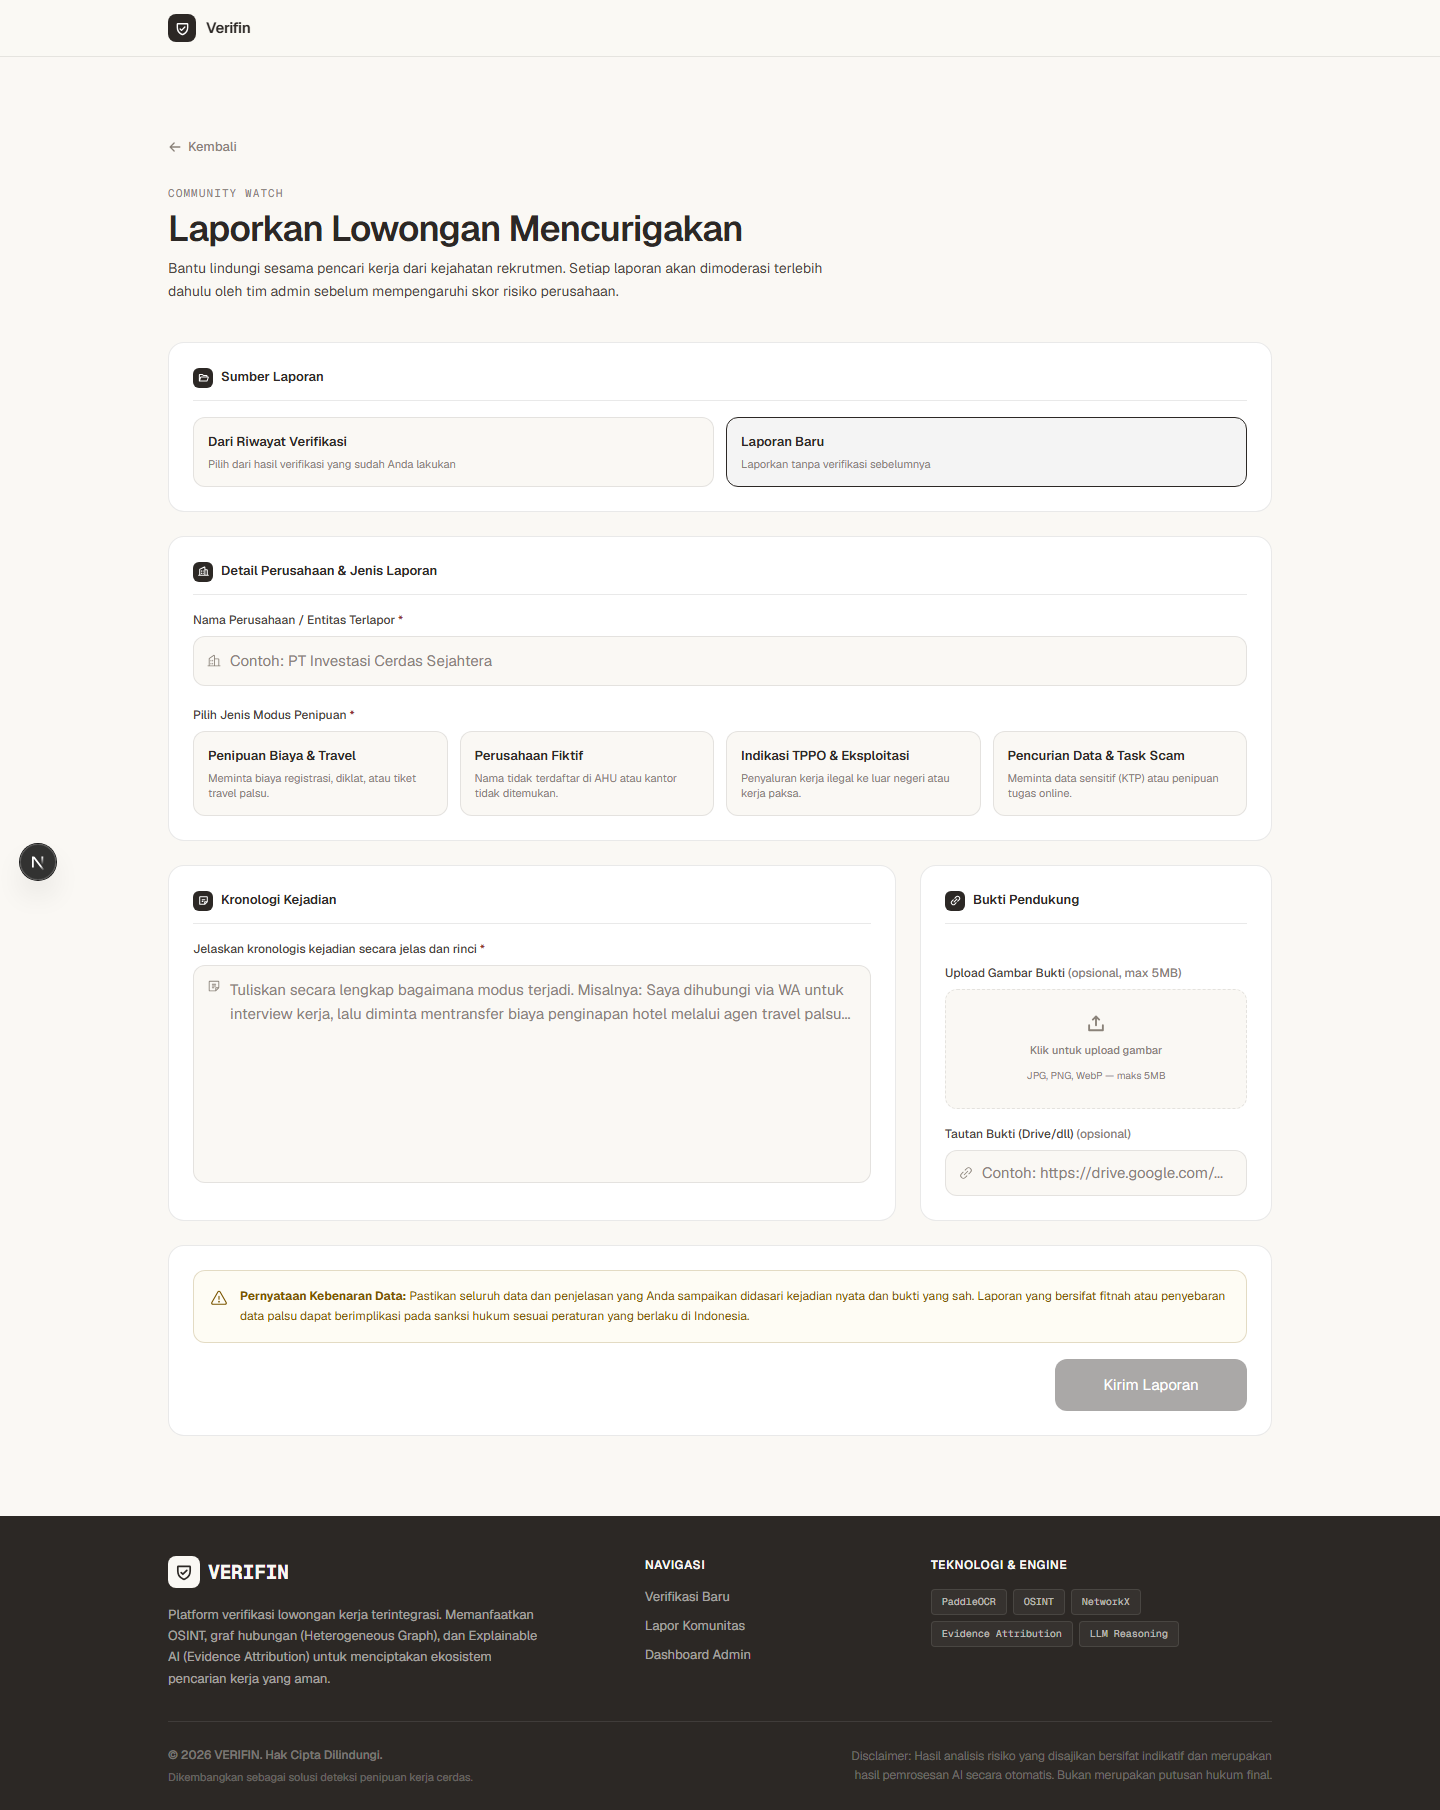
\includegraphics[width=\linewidth]{images/mockup-riwayat.png}
    \label{fig:mockup-riwayat}
  \end{subfigure}
  \caption{Halaman Komunitas dan Riwayat Verifikasi}
  \label{fig:halaman-pendukung}
\end{figure}

\refstepcounter{section}
\section*{BAB VIII\quad DOKUMENTASI CARA PENGGUNAAN}
\addcontentsline{toc}{section}{BAB VIII DOKUMENTASI CARA PENGGUNAAN}

\subsection*{A.\quad Persyaratan Akses dan Langkah Penggunaan}
\addcontentsline{toc}{subsection}{A. Persyaratan Akses dan Langkah Penggunaan}

\begin{enumerate}[label=\textbf{\arabic*.}]
  \item Perangkat dengan browser modern (Chrome, Firefox, Edge, Safari versi terkini)
  \item Koneksi internet untuk menjalankan pipeline OSINT dan LLM
  \item Tidak diperlukan akun atau registrasi untuk verifikasi dasar
\end{enumerate}

Langkah penggunaan: (1) Buka aplikasi Verifin di browser; (2) Masukkan data lowongan via tiga kanal: teks (salin-tempel), gambar/poster (unggah JPG/PNG/WebP untuk OCR), atau tautan (URL halaman lowongan); (3) Klik \textbf{``Verifikasi Sekarang''} dan tunggu modal progres menampilkan tahapan: OCR/Ekstraksi Entitas $\to$ Investigasi OSINT $\to$ Analisis Graf Jaringan $\to$ Sintesis LLM \& XAI (1--2 menit); (4) Baca hasil: verdict (AMAN/WASPADA/BAHAYA), Skor Risiko 0--100, ringkasan naratif LLM, breakdown XAI, detail OSINT, dan graf jaringan penipuan; (5) Tindak lanjut sesuai verdict: AMAN=tetap verifikasi mandiri, WASPADA=verifikasi lanjutan, BAHAYA=jangan respon + laporkan.

\subsection*{B.\quad Fitur Pelaporan Komunitas dan Riwayat}
\addcontentsline{toc}{subsection}{B. Fitur Pelaporan Komunitas dan Riwayat}

Pengguna dapat melaporkan entitas mencurigakan (nomor HP, email, URL, nama perusahaan) melalui halaman \textbf{Komunitas}. Laporan diverifikasi dan diintegrasikan ke graf jaringan penipuan. Seluruh verifikasi dapat diakses kembali via halaman \textbf{Riwayat} yang menampilkan verdict, skor risiko, dan waktu pemeriksaan.

\section*{DAFTAR PUSTAKA}
\addcontentsline{toc}{section}{DAFTAR PUSTAKA}

\begingroup
\footnotesize
\begin{enumerate}[label={[\arabic*]}, labelindent=0pt, leftmargin=0.95cm, labelwidth=0.60cm, labelsep=0.35cm, align=left, itemsep=3pt, parsep=0pt, topsep=2pt]

\item Badan Pusat Statistik (BPS), ``Keadaan Ketenagakerjaan Indonesia Februari 2025,''
  \textit{Berita Resmi Statistik No.\ 39/05/Th.\ XXVIII}, Mei 2025. [Daring]. Tersedia: \url{https://www.bps.go.id}

\item Global Anti-Scam Alliance (GASA) \& Mastercard, ``State of Scams in Indonesia 2024,''
  \textit{GASA Annual Report}, 2024. [Daring]. Tersedia: \url{https://www.gasa.org}

\item Kementerian Luar Negeri Republik Indonesia (Kemenlu RI), ``Penanganan WNI Korban
  \textit{Online Scamming} dan TPPO di Asia Tenggara,'' \textit{Direktorat Perlindungan WNI dan BHI},
  2024.

\item United Nations Office on Drugs and Crime (UNODC), ``Casinos, Cyber Fraud, and Trafficking
  in Persons for Forced Criminality in Southeast Asia,'' \textit{UNODC Regional Report}, 2023.

\item S.\ Shalini, R.\ Lokesh, and S.\ Priya, ``Fake Job Posting Detection Using Machine
  Learning,'' \textit{International Journal of Computer Applications}, vol.\ 183, no.\ 52,
  pp.\ 1--6, 2022.

\item T.\ Alwafi and R.\ Abdulrahman, ``Detection of Recruitment Fraud Using Semantic
  Approaches,'' \textit{Security and Communication Networks}, vol.\ 2019, Art.\ ID 7523043, 2019.
  doi: \href{https://doi.org/10.1155/2019/7523043}{10.1155/2019/7523043}.

\item V.\ G.\ Varsha and P.\ A.\ Thomas, ``Explainable AI For Phishing Detection: Techniques,
  Challenges, and Experimental Validation,'' in \textit{Proc.\ IEEE Recent Advances in
  Intelligent Computational Systems (RAICS)}, Nov.\ 2025.

\item J.\ Pastor-Galindo, P.\ Nespoli, F.\ G.\ Marmol, and G.\ M.\ Perez, ``The Not Yet
  Exploited Goldmine of OSINT: Opportunities, Open Challenges and Future Trends,''
  \textit{IEEE Access}, vol.\ 8, pp.\ 10282--10304, 2020.
  doi: \href{https://doi.org/10.1109/ACCESS.2020.2965257}{10.1109/ACCESS.2020.2965257}.

\item B.\ Wilie et al., ``IndoNLU: Benchmark and Resources for Evaluating Indonesian Natural
  Language Understanding,'' in \textit{Proc.\ 1st Conf.\ of the Asia-Pacific Chapter of the
  Association for Computational Linguistics (AACL)}, Dec.\ 2020, pp.\ 843--857.

\end{enumerate}
\endgroup

\end{document}
